\documentclass[ignorenonframetext,xcolor=pdftex,dvipsnames,table]{beamer}
\mode<article>{\usepackage[svgnames]{xcolor}
\usepackage[colorlinks=true]{hyperref}
\setlength{\textwidth}{180mm}
\setlength{\oddsidemargin}{-1cm}
\setlength{\evensidemargin}{-1cm}
%\setlength{\topmargin}{-40pt}
}
\mode<presentation>{
\usetheme{Madrid}
\setbeamercovered{transparent}
% or whatever (possibly just delete it)
%\AtBeginSubsection[]
%{
%  \begin{frame}<beamer>{Outline}
%    \tableofcontents[currentsection,currentsubsection]
%  \end{frame}
%}
%%%Configure section names to appear in beamer
\setbeamertemplate{headline}
{%
\begin{beamercolorbox}{section in head/foot}
\vskip2pt\insertsection$\to$\insertsubsection\vskip2pt
\end{beamercolorbox}%
}
%\usepackage[svgnames]{xcolor}
%%paginacion
\usefoottemplate{\hfill \insertframenumber{}}% /\inserttotalframenumber}
%delete the navigation buttons
\setbeamertemplate{navigation symbols}{}
}
% everyone:

\usepackage[utf8]{inputenc}
%\usepackage{textcomp}
\usepackage[spanish]{babel}
\spanishdecimal{.}
\addto\captionsspanish{%
\def\tablename{Tabla}%
}
\usepackage{amsmath}
\usepackage{amssymb}
\usepackage{amsthm}
%%%%%%%%%%from beyond.tex
\usepackage{cancel}
\usepackage{simplewick}
\usepackage[toc,page]{appendix}
%%%%%%%%%
\usepackage{siunitx} 
\sisetup{group-minimum-digits=4} %compatibility with PDG
%%%%%%%%%%%%%
\newcommand{\timesm}{\times}
\newcommand{\pmm}{\pm}
\newcommand{\mpm}{\mp}

\usepackage{comment}
\includecomment{inprogress}
\specialcomment{inprogress}
{\begingroup\itshape \textbf{Begin Draft:}}{\textbf{End Draft.} \medskip \endgroup}
%\excludecomment{inprogress}

\includecomment{inprogress}
\specialcomment{inprogress}
{\begingroup\itshape \textbf{Begin Draft:}}{\textbf{End Draft.} \medskip \endgroup}
\excludecomment{inprogress}

\includecomment{borrar}
\specialcomment{borrar}
{\begingroup\itshape \textbf{Begin Draft:}}{\textbf{End Draft.} \medskip \endgroup}
\excludecomment{borrar}

\includecomment{details}
\specialcomment{details}
{\begingroup}{\endgroup}
%\excludecomment{details}
%\PreviewEnvironment{details}
%%%%%%%%%%%%%%%%%%%%%%%%%%%%%%

\includecomment{english}
\specialcomment{english}
{\begingroup}{\endgroup}
\excludecomment{english}
%%%%%%%%%%%%%%%%%%%%%%%%
\includecomment{spanish}
\specialcomment{spanish}
{\begingroup}{\endgroup}
%\excludecomment{spanish}


\def\lt{<} % compatibility with instiki
\def\gt{>} % compatibility with instiki
%%%%%%%%%%%%%%%%%%%%%%
%\usepackage[colorlinks=true]{hyperref}
\usepackage{graphicx}
%\usepackage{color}
\usepackage{bm}
\usepackage{framed}
\definecolor{shadecolor}{named}{gray}
\newcommand{\filetitle}[1]{
\begin{shaded}
\noindent{\color{white}#1}
\end{shaded}}


\graphicspath{{figures/}}
%%%%%%%%%%%%%%%%%%%%listings%%%%%%%%%%%%%%%
\usepackage{listings}
%\usepackage{listingsutf8}

\usepackage{caption}
\DeclareCaptionFont{white}{\color{white}}
\DeclareCaptionFormat{listingm}{\colorbox{gray}{\parbox{\textwidth}{#1#2#3}}}
\DeclareCaptionFormat{listingmm}{\colorbox{gray}{\parbox{\textwidth}{Hola #3}}}
\DeclareCaptionFormat{ipython}{\colorbox{lightgray}{\parbox{\textwidth}{\centering IPython}}}
\DeclareCaptionFormat{terminal}{\parbox[t]{\textwidth}{\centering \fbox{Terminal}}}
\captionsetup[lstlisting]{format=listingm,labelfont=white,textfont=white}
%%%%%%%%%%%%%%%%%%%%%%%%%%%%%%%%%%%%%%%%%%
%\usepackage{bbold}
\newenvironment{pyprogram}{\captionsetup[lstlisting]{format=listingm,labelfont=white,textfont=white}
\lstset{frame=bl}}
{}
\newenvironment{pysnippet}{\captionsetup[lstlisting]{format=listingm,labelfont=white,textfont=white}}{}
\newenvironment{ipython}{\captionsetup[lstlisting]{format=ipython}
\lstset{columns=fixed}}{}
\newenvironment{pysample}{\captionsetup[lstlisting]{format=ipython}
\lstset{frame=tb}
}{}
\newenvironment{terminal}{\captionsetup[lstlisting]{format=terminal}
\lstset{language=bash,backgroundcolor=\color{lightgray},belowcaptionskip=-0pt,columns=fixed}
}{}
%\newenvironment{ejemplo}{}{}

 \lstset{language=python
%,inputencoding=utf8
%,showspaces=false
%{\small Hola} {\footnotesize Hola} {\scriptsize Hola} {\tiny Hola}
,basicstyle=\small\ttfamily
%,basicstyle=\small\sffamily,
,keywordstyle=\color{blue}
,commentstyle=\normalfont\ttfamily\color{red}
,stringstyle=\color{Green}
%,numbers=left
%,numberstyle=\tiny
,frame=b
,inputencoding=utf8
,extendedchars=true
,columns=fullflexible
,showstringspaces=false
%,backgroundcolor=\color{lightgray}
,texcl=true
}

\newtheorem{ejemplo}[theorem]{Ejemplo}

\newcommand{\chapter}{}
\newcommand{\ignore}[1]{}
\begin{document}
%%Comment the following two lines for full processing
%\mode<presentation>{\input{cf_tmp}}
%\end{document}

\mode<presentation>{%instiki:category: FisicaSubatomica
%http://localhost:2500/wiki/show/Cap%C3%ADtulo+II
%% Ilustrar como el teorema de Noether es el mismo
%% para el caso local que global
\chapter{Campos bosónicos}
\label{cha:campos-vectoriales} %noinstiki
%instiki:
%instiki:***
%instiki:
%instiki:[[NotasFS|Tabla de Contenidos]]
%instiki:
%instiki:***
%generated with html2itexTOC instiki_source.html
%instiki:
%instiki:* [Unidades Naturales](#NU)
%instiki:
%instiki:* [Notaci\'on relativista](#srn)
%instiki:
%instiki:  * [Ejemplos de cuadrivectores](#ejemplos_de_cuadrivectores)
%instiki:
%instiki:  * [Ecuaciones covariantes](#ecuac-covar)
%instiki:
%instiki:* [Ecuaciones de Maxwell en notaci\'on covariante](#maxeqs)
%instiki:
%instiki:  * [Lagrangiano Electromagn\'etico](#lagr-electr)
%instiki:
%instiki:  * [Energ\'\i a del campo electromagn\'etico](#energa_del_campo_electromagntico)
%instiki:
%instiki:  * [Fijaci\'on del gauge](#fijacion-del-gauge)
%instiki:
%instiki:* [Ecuaciones de Proca](#ecuacion-de-proca)
%instiki:
%instiki:* [Problemas](#problemas2)
%instiki:
%instiki:***
%instiki:

 Se mostrará como la invarianza de la Acción bajo transformaciones es el punto de partida en la construcción de densidades Lagrangianas únicas.

%\subsection{Transformaciones de Lorentz}
%\label{sec:transf-de-lorentz}



 

\section{Construción de Lagrangianos covariantes}
En está sección vamos a conectar la discusión sobre el Lagrangiano de las vibraciones de la cuerda con las tranformaciones de Lorentz de la relatividad especial. Dicho Lagrangiano tiene hasta ahora la siguiente dependencia funcional $\mathcal{L}(\partial_{\mu}\phi)$.

En la formulación de la teoría clásica de campos debemos asegurarnos de que todos los términos posibles perimtidos por la simetrías asociadas al campo estén presentes en la densidad Lagrangiana. De inmediato surge la pregunta: ¿Qué posibles términos de la forma $\partial_{\mu}\phi$ podrían estar presentes en Lagrangiano?. Antes de responder está pregunta, abordemos el problema algo más general donde la densidad Lagrangiana también depende del campo como mismo
\begin{align*}
  \mathcal{L}(\phi,\partial_\mu \phi)\,.
\end{align*}
En la ecuación~\eqref{eq:dlc3d}, teníamos un Lagragiano en función de $\partial_{\mu}\phi$, y haciendo $v\to c=1$, tenemos
\begin{align}
\label{eq:Lpr}
  \mathcal{L}(\partial_{\mu}\phi)
    =&\frac{1}{2}\left[
      {\partial_0\phi}\,{\partial_0\phi}-\sum_i{\partial_i\phi}\,{\partial_i\phi}
   \right]\nonumber\\
    =&\frac{1}{2}\left[
      {\partial_0\phi}\,{\partial^0\phi}+{\partial_i\phi}\,{\partial^i\phi}
   \right]\nonumber\\
   =&\frac{1}{2}{\partial_\mu\phi}\,{\partial^\mu\phi}\,.
\end{align}
donde se ha usado la convención de suma para índices repetidos. Note que para que la velocidad de propagación sea independiente del sistema de coordenadas se requiere su identificación con la velocidad de la luz. De modo que la queremos interpretar los términos de la densidad Lagrangiana como objetos invariantes, necesariamente se tiene que hacer en el contexto de la relatividad especial.


\section{Transformación de Lorentz para campos escalares}

El campo escalar esta definido por sus propiedades bajo transformaciones de Lorentz. Vamos a estudiar el comportamiento de un campo escalar bajo una transformación general de Lorentz:
\begin{align}
\label{eq:179qft}
  x^\mu\to {x'}^\mu={\Lambda^\mu}_\nu x^\nu\,,
\end{align}
Por definición, el campo escalar no cambia bajo la transformación de Lorentz, es decir, su forma funcional queda inalterada. Por consiguiente el campo escalar debe satisfacer que
\begin{align}
 \phi(x)\to  \phi'(x')=\phi(x)\,,
\end{align}
como se ilustró en la Fig.~\ref{fig:trasla}. La prima en $\phi$ representa el cambio intrínseco en el campo $\phi$ como consecuencia de la transformación.


Usando la ec.~\eqref{eq:179qft}, tenemos que
\begin{align}
    \phi'(x')=\phi(\Lambda^{-1}x')\,.
\end{align}
Esto es, el campo transformado, evaluado en el punto transformado, da el mismo valor que el campo evaluado en el punto antes de la transformación. 

\begin{frame}[fragile,allowframebreaks]

%Therefore, for an arbitrary space-time point we have that the scalar field transforms under a Lorentz transformation as
Por consiguiente, para un punto del espacio tiempo arbitrario tenemos
que el campo escalar transforma bajo una transformación de Lorentz como
\begin{align}
  \label{eq:scalarlorentz}
 \phi(x)\to  \phi'(x)=\phi(\Lambda^{-1}x)\,.
\end{align}
\end{frame}



% Definimos el cambio correspondiente como
% \begin{align}
%   \delta \phi(x)=\phi'(x)-\phi(x)\,.
% \end{align}




Para comprobar la invarianza de Lorentz de la Acción para el campo escalar, necesitamos las propiedades de transformación para $\partial_\mu$. En conveniente invertir la ec.~\eqref{eq:179qft}
\begin{align}
  {\left(\Lambda^{-1}\right)^\mu}_\alpha{x'}^\alpha=&{\left(\Lambda^{-1}\right)^\mu}_\alpha{\Lambda^\alpha}_\nu x^\nu\nonumber\\
=&\delta^\mu_\nu x^\nu\nonumber\\
=&x^\mu\,,
\end{align}
\begin{align}
  \frac{1}{{x'}^\nu}= {\left(\Lambda^{-1}\right)^\mu}_\nu\frac{1}{x^\mu}\,,
\end{align}
o
\begin{align}
  \label{eq:183qft}
    \frac{1}{{x'}^\mu}= {\left(\Lambda^{-1}\right)^\nu}_\mu\frac{1}{x^\nu}\,,
\end{align}
de modo que la transformación de Lorentz para $\partial_\mu=\partial/\partial x^\mu$, es
\begin{align}
  \label{dmulrtran}
   \frac{\partial}{{\partial x'}^\mu}=& {\left(\Lambda^{-1}\right)^\nu}_\mu\frac{\partial}{\partial x^\nu}\nonumber\\
   {\partial\,}'_\mu=& {\left(\Lambda^{-1}\right)^\nu}_\mu\partial_\nu\,,
\end{align}
Podemos ahora demostrar que la Acción obtenida del Lagrangiano en la ec.\eqref{eq:Lpr} es invariante bajo transformaciones de Lorentz haciendo uso de la ec.~(\ref{eq:Lambdacontra}). Para hacer la demostración más general, podemos agregar una función general que solo dependa del campo $\phi$ pero no de sus derivadas, $V(\phi)$
\begin{align}
  \mathcal{L}(\phi(x),\partial_{\mu}\phi(x))\to  \mathcal{L}'=& \frac{1}{2}\partial'_\mu\phi'(x)\partial^{'\mu}\phi'(x)-V(\phi'), \nonumber\\
  =&{\left(\Lambda^{-1}\right)^\nu}_\mu g^{\mu \rho}{\left(\Lambda^{-1}\right)^\sigma}_\rho \partial_\nu\phi(\Lambda^{-1}x) \partial_\sigma \phi(\Lambda^{-1}x) -V(\phi')\nonumber\\
  =& g^{\nu \sigma}\partial_\nu\phi(\Lambda^{-1}x) \partial_\sigma \phi(\Lambda^{-1}x) -V(\phi(\Lambda^{-1}x))\nonumber\\
  =& \partial_\nu\phi(\Lambda^{-1}x) \partial^{\nu} \phi(\Lambda^{-1}x) -V(\phi(\Lambda^{-1}x)) \nonumber\\
  =&\mathcal{L}(\phi(\Lambda^{-1}x),\partial_{\mu}\phi(\Lambda^{-1}x))\,.
\end{align}
Ya que la Acción involucra la integración sobre todos los puntos, esta es invariante bajo transformaciones de Lorentz. Explícitamente
\begin{align}
  S\to S'=\int d^4x\, \mathcal{L}
\end{align}

Note que en unidades naturales
\begin{align}
  [S]=[\hbar]=1,
\end{align}
y ya que $[d^4x]=E^{-4}$, entonces
\begin{align}
  [\mathcal{L}]=E^{4}\,.
\end{align}
Como $[\partial_{\mu}]=E$, entonces
\begin{align}
  [\phi]=E\,.
\end{align}


 
\section{Principio de mínima acción para campos}
Hemos visto que la acción para una oscilación mecánica en tres dimensiones se puede escribir en una notación similar a la del producto escalar de un cuadrivector de Lorentz $\partial_\mu\phi$. Cuando dicho campo se interpreta como un campo fundamental, es decir, que su velocidad de propagación es independiente de los sistemas de referencia inerciales, entonces la Acción queda invariante bajo dicho producto escalar. También hemos visto que adicionar una función del campo $V(\phi)$, la invarianza de la acción se mantiene.

Establecemos el \emph{principio de mínima acción para campos} de la siguiente manera: La acción más general posible para un conjunto de campos contiene todos los posibles productos escalares entres los campos y sus derivadas, con las siguientes restricciones
\begin{enumerate}
\item La dimensión de los campos y derivadas en cada término de la correspondiente densidad lagrangiana debe ser menor o igual a cuatro.
\item La densidad Lagrangiana no debe contener derivadas altas (máximo dos derivadas)
\item Los campos fundamentales se deben anular a espacio infinito.
\end{enumerate}
Con estas restricciones es suficiente mantener los primeros cuatro términos de la expansión de Taylor de $V(\phi)$ (el término constante se puede remover redefiniendo el estado de mínima energía)
\begin{align}
  \label{eq:fullV}
  V(\phi)=a \phi + b\phi^2+c\phi^3+d\phi^4\,,
\end{align}

La última condición excluye términos del tipo
\begin{align}
  \partial_\mu \partial^\mu \phi\,,   \phi\partial_\mu \partial^\mu \phi\,.
\end{align}
De modo que la densidad Lagrangiana más general posible para un campo escalar real es
\begin{align}
  \frac{1}{2}{\partial_\mu\phi}\,{\partial^\mu\phi}-V(\phi)\,.
\end{align}
La ecuación de movimiento es
\begin{align}
  \left( \partial_\mu \partial^{\mu} +2b \right)\phi= J(\phi)\,,
\end{align}
donde
\begin{align}
  J(\phi)=- \left( a + 3c\phi^3 + 4d\phi^4 \right),
\end{align}
es el término de fuente. En ausencia de fuentes el campo $\phi$ se propaga libremente a través de la ecuación
\begin{align}
  \left( \partial_\mu \partial^{\mu} +2b \right)\phi= 0.
\end{align}

A continuación procedemos a encontrar una interpretación física al coeficiente $2b$
\subsection{Ecuaciones covariantes}
\label{sec:ecuac-covar}


Con el cuadrivector \eqref{eq:cv_hatpmu} podemos construir la
siguiente ecuaci\'on
\begin{align}
  \hat{p}_\mu\hat{p}^\mu\phi&=m^2\phi\nonumber\\
  i\partial_\mu i\partial^\mu\phi&=m^2\phi\nonumber\\
  -\partial_\mu\partial^\mu\phi&=m^2\phi\nonumber\\
  \label{eq:waveec}
  \left(\frac{\partial^2}{\partial t^2}-\nabla^2+m^2\right)\phi&=0.
\end{align}
Que corresponde a la ecuaci\'on de Klein-Gordon \eqref{eq:152}. Una expresi\'on escrita en t\'erminos de productos escalares de Lorentz se dice que esta en \emph{forma covariante}. El Lagrangiano covariante que da lugar a
\'esta ecuaci\'on es (ver ec. \eqref{eq:150}
\eqref{eq:15}). %noinstiki[in Cap. I](/wiki/show/Cap%C3%ADtulo+I#eq:15)). 

\begin{equation}
  \label{eq:wavelagtrue}
  \mathcal{L}=\frac{1}{2}\partial_\mu\phi\partial^\mu\phi-\frac{1}{2}m^2\phi^2
\end{equation}
El Lagrangiano m\'as general posible para el campo $\phi$ es en general bastante arbitrario:
\begin{equation}
  \mathcal{L}=\frac{1}{2}\partial_\mu\phi\partial^\mu\phi-V(\phi)\,,
\end{equation}
donde $f(\phi)$ es una función de campos escalar real $\phi$. Si $V(\phi)$ es una función polinómica del campo $\phi$, tenemos por ejemplo.
\begin{equation}
  \label{eq:wavelag}
  \mathcal{L}=\frac{1}{2}\partial_\mu\phi\partial^\mu\phi-\frac{1}{2}m^2\phi^2-\frac{1}{4}\lambda\phi^4-a\phi+b\phi^3.
\end{equation}

En asencia de fuentes $a=c=d=0$ en la ec.~\eqref{eq:fullV}, y usando las
ecuaciones de Euler-Lagrange \eqref{eq:eelcallfmu}, se obtiene
\begin{align}
  (\hat{p}_\mu\hat{p}^\mu-m^2)\phi&=0\nonumber\\
  \label{eq:k-gpmu} %noinstiki
(\hat{E}^2-\hat{\mathbf{P}}^2-m^2)\phi&=0\\
\label{eq:kg} 
  (\Box+m^2)\phi&=0,
\end{align}
donde
\begin{equation}
  \label{eq:dalambertiano}
  \Box\equiv\partial_\mu\partial^\mu=\frac{\partial^2}{\partial t^2}-\nabla^2. 
\end{equation}
Es el D'Alembartiano~\cite{daelembertiano}. 
Ec.~\eqref{eq:k-gpmu} %noinstikiEc.~\eqref{eq:kg}
corresponde a la forma de operadores de la
ecuaci\'on de energ\'\i a-momentum relativista. La
ec.~\eqref{eq:kg} se conoce como la ecuaci\'on de Klein-Gordon, con
Lagrangiano
\begin{equation}
  \label{eq:kglag}
  \mathcal{L}=\frac{1}{2}\partial_\mu\phi\partial^\mu\phi-\frac{1}{2}m^2\phi^2, 
\end{equation}
Una expresi\'on escrita en t\'erminos de productos escalares de
Lorentz se dice que esta en \emph{forma covariante}. Por lo tanto la
ecuaci\'on de Klein--Gordon y su correspondiente Lagrangiano est\'an
en forma covariante. Tambi\'en tienen la simetr\'\i a
$\phi\to-\phi$. A $\phi$ se le denomina \emph{campo escalar}.

Hemos identificado que el término $2a=m^2$ se podría interpretar como la masa al cuadrado del campo escalar. Dicha interpretación surge de analizar la segunda cuantización del campo $\phi$ que se traduce en una interpretación en términos del oscilador armónico.
%TODO: FALTA

Realizaciones propuestas para este campo escalar incluye el de un campo de materia oscura con un potencial tipo oscilador armónico.
% figura
Pero una realización ya encontrada en la naturaleza corresponde al campo de Higgs con un potencial tipo ruptura expontánea de vacio

Una realización física para la acción del campo escalar real con un potencia escalar tipo ``slow-roll''  corresponde al campo del inflatón en cosmología.




\section{Lagrangiano para el campo vectorial}
\begin{frame}[fragile,allowframebreaks]
Ya estamos en capacidad de responder la siguiente pregunta: ¿Cual es el Lagrangiano más general posible para el campo de cuatro componentes $A^{\mu}(x)$ compatible con la invarianza de Lorentz 

Las correspondientes transformaciones son

\begin{align}
  A^\mu(x)\to {A'}^\mu(x')={\Lambda^\mu}_\nu A^\nu(\Lambda^{-1}x)\,.
\end{align}


\begin{align}
\label{eq:172qft}
  A^\mu\to{A'}^\mu=A^\mu-\partial^\mu\chi(x)\;?
\end{align}




Definiendo
\begin{align*}
  F^{\mu\nu}&=\partial^\mu A^\nu-\partial^\nu A^\mu\\
  G^{\mu\nu}&=\partial^\mu A^\nu+\partial^\nu A^\mu\\
\end{align*}
El Lagrangiano que da lugar a una Acción invariante de Lorentz para el cuadrivector $A^\mu$
es, hasta derivadas totales y potencias en los campos de hasta dimensión 4:
\begin{align}
  \mathcal{L}=&-\frac{1}{4}F^{\mu\nu}F_{\mu\nu}-\frac{1}{4}G^{\mu\nu}G_{\mu\nu}-\frac{1}{2}F^{\mu\nu}G_{\mu\nu}\nonumber\\
&-J^\mu A_\mu+
 \frac{1}{2}m^2A^\mu A_\mu +\lambda_1\partial_\nu A^\nu(x) A_\mu(x) A^\mu(x)+\lambda_2 A^\mu A_\mu A^\nu A_\nu\nonumber\\
&+\lambda_3 F^{\mu\nu}(x)A_\mu(x) A_\nu(x)+\lambda_4G^{\mu\nu}(x)A_\mu(x) A_\nu+\cdots
  \label{eq:lagAmu}
\end{align}
\end{frame}

\begin{itemize}
\item \textbf{Ejercicio:} Show that terms like $\partial^\mu A^\nu(x)\partial_\mu A_\nu(x)$, and hence $F^{\mu\nu}F_{\mu\nu}$, transforms as
  \begin{align}
    \partial^\mu A^\nu\left(\Lambda^{-1}x\right)\partial_\mu A_\nu\left(\Lambda^{-1}x\right)
  \end{align}
Hint: use the Lorentz transformation properties of $\partial_\mu$ in eq.~\eqref{dmulrtran}.
\end{itemize}
In the case of $J^\mu A_\mu$:
\begin{align}
  J^\mu(x)A_\mu(x)\to g_{\mu\nu}{J'}^\mu(x){A'}^\nu(x)=& g_{\mu\nu}{\Lambda^\mu}_\rho J^\rho\left(\Lambda^{-1}x\right){\Lambda^\nu}_\sigma A^\sigma\left(\Lambda^{-1}x\right)\nonumber\\
=& {\Lambda^\mu}_\rho g_{\mu\nu}{\Lambda^\nu}_\sigma J^\rho\left(\Lambda^{-1}x\right)A^\sigma\left(\Lambda^{-1}x\right)\nonumber\\
=& g_{\rho\sigma}J^\rho\left(\Lambda^{-1}x\right)A^\sigma\left(\Lambda^{-1}x\right)\,,
\end{align}
in the case $\partial_\nu A^\nu(x) A_\mu(x) A^\mu(x)$:
\begin{align}
   \partial_\nu A^\nu(x) A_\mu(x) A^\mu(x)\to {\partial'}_\nu{A'}^\nu(x') {A'}_\mu(x') {A'}^\mu(x')=& {\left(\Lambda^{-1}\right)^\sigma}_\nu{\Lambda^\nu}_\rho\partial_\sigma A^\rho\left(\Lambda^{-1}x\right) A_\mu\left(\Lambda^{-1}x\right) A^\mu\left(\Lambda^{-1}x\right)\nonumber\\
=& \delta^\sigma_\rho\partial_\sigma A^\rho\left(\Lambda^{-1}x\right) A_\mu\left(\Lambda^{-1}x\right) A^\mu\left(\Lambda^{-1}x\right)\nonumber\\
=& \partial_\rho A^\rho\left(\Lambda^{-1}x\right) A_\mu\left(\Lambda^{-1}x\right) A^\mu\left(\Lambda^{-1}x\right)\,,\nonumber\\
\end{align}
and similarly for the other terms. Under a Lorentz transformation the full Lagrangian transform as
\begin{align}
  \mathcal{L}(x)\to\mathcal{L}'(x)=\mathcal{L}(\Lambda^{-1}x) 
\end{align}
Since the Action involves the integration over all the points, it is invariant under the Lorentz transformation. The $J^\mu(x)$ does not involves the introduction a new vector field, because it will be identified later as the 4--current.


Terms like
\begin{align}
  K_\nu A^\nu(x) A_\mu(x) A^\mu(x)\,,
\end{align}
(for $K_\nu$ constant) are not Lorentz invariant:
\begin{align}
  K_\nu A^\nu(x) A_\mu(x) A^\mu(x)\to K_\nu{A'}^\nu(x) {A'}_\mu(x) {A'}^\mu(x)=& K_\nu{\Lambda^\nu}_\rho A^\rho\left(\Lambda^{-1}x\right) A_\mu\left(\Lambda^{-1}x\right) A^\mu\left(\Lambda^{-1}x\right)\,.
\end{align}
$K_\nu(x)A^\nu(x)A_\mu(x)A^\mu(x)$ is Lorentz invariant %but not gauge-invariant (see below).




%\begin{frame}[fragile,allowframebreaks]
% The field $A^\mu(x)$ transforms simultaneously as field and as vector under Lorentz transformation
% \begin{align}
%   A^\mu(x)\to {A'}^\mu(x')={\Lambda^\mu}_\nu A^\nu(\Lambda^{-1}x)\,.
% \end{align}
% \end{frame}




\section{Lagrangiano electromagnético}
Las ecuaciones de Maxwell tienen la siguiente simetría
\begin{align}
   A^\mu\to {A'}^\mu=&A^\mu-\partial^\mu\theta(x)
\end{align}
 que cuando fue descubierta parecía ser una simple curiosidad matemática de dichas ecuaciones.

Comparando con la transformación más general de un campo vemos que para el campo vectorial con dicha invarianza $a_i=0$ y $b^{\mu_i}=1$ en la ec.\eqref{eq:infdt}. 

Ya estamos en capacidad de responder la siguiente pregunta: ¿Cual es el Lagrangiano más general posible para el campo de cuatro componentes $A^{\mu}(x)$ compatible con la invarianza de Lorentz y la invarianza bajo transformaciones gauge?


De hecho, si aplicamos el segundo teorema de Noether al campo de radiación
\begin{align}
  0=&\partial_{\mu} \left( \mathcal{E}_3 b^{\mu}_3 \right) \nonumber\\
   0=&\partial_{\mu} \left( \mathcal{E}_3 \delta^{\mu}_\nu \right) \nonumber\\
   0=&
 \partial_{\mu} \partial_{\rho} \left[ \frac{\partial \mathcal{L}}{\partial \left(  \partial_{\rho} A_{\nu}\right)}  \delta^{\mu}_\nu \right] - \partial_{\mu} \frac{\partial \mathcal{L}}{\partial A_{\nu}}\delta^{\mu}_{\nu} \nonumber\\
   0=&
 \partial_{\mu} \partial_{\rho}\left[ \frac{\partial \mathcal{L}}{\partial \left(  \partial_{\rho} A_{\mu}\right)}  \right] - \partial_{\mu} \frac{\partial \mathcal{L}}{\partial A_{\mu}} \,.
\end{align}
El segundo témrino da lugar a la misma corriente conservada fermiónica
\begin{align}
  \partial_{\mu} \frac{\partial \mathcal{L}}{\partial A_{\mu}}=&
\partial_{\mu} j^{\mu}=0\,,
\end{align}
Por consiguiente, la identidad resultante
\begin{align}
   \partial_{\mu} \partial_{\rho}\left[ \frac{\partial \mathcal{L}}{\partial \left(  \partial_{\rho} A_{\mu}\right)}  \right]=0\,,
\end{align}
se puede interpretar como la necesidad de introducir el tensor antisimétrico
\begin{align}
  F_{\mu\nu}=\frac{\partial \mathcal{L}}{\partial \left(\partial  \partial_{\nu} A_{\mu}\right)}\,,
\end{align}
tal que
\begin{align}
  \partial_{\mu}\partial_{\nu}F^{\mu\nu}=0\,.
\end{align}
Para obtener una forma para $F_{\mu\nu}$, es conveniente imponer que la densidad Lagrangiana asociada sólo a las nuevas contribuciones de los campos $A_{\nu}$ y sus derivadas $\partial_{\mu}A_{\nu}$, denotada como $\mathcal{L}_{\text{EM}}$ 
%en la ec.
sea invariante gauge local bajo la transformación del campo $A_{\mu}$ en \eqref{eq:tfgl}. Esto implíca que $\mathcal{L}_{\text{EM}}$  solo puede depender de las derivadas de las campos, y por consiguiente $F^{\mu\nu}$ debe ser una combinación antisimétrica de las derivadas de los campos
\begin{align}
  F_{\mu\nu}\equiv\partial_{\mu}A_{\nu}-\partial_{\nu}A_{\mu}\,.
\end{align}
Con esta definición, bajo la transformación  \eqref{eq:tfgl}
\begin{align}
  F_{\mu\nu}\to F_{\mu\nu}'=F_{\mu\nu}\,.
\end{align}
Por consiguiente, el único término posible que a la vez es invariante de Lorentz e invariante gauge local es
\begin{align}
  \mathcal{L}_{\text{EM}}=-\frac{1}{4}F_{\mu\nu}F^{\mu\nu}\,.
\end{align}
%%hablar de la ecuaciones de Euler-Lagrange, el gauge de Lorentz y la ecuación de onda.


Podemos coprobar que si
\begin{align}
F^{\rho\sigma}F_{\rho\sigma}=&(\partial^\rho A^\sigma-\partial^\sigma A^\rho)(\partial_\rho A_\sigma-\partial_\sigma A_\rho)\nonumber\\
=&\partial^\rho A^\sigma\partial_\rho A_\sigma-\partial^\rho A^\sigma\partial_\sigma A_\rho-\partial^\sigma A^\rho\partial_\rho A_\sigma+\partial^\sigma A^\rho\partial_\sigma
A_\rho\nonumber\\
=&g^{\rho\alpha}g^{\sigma\beta}(\partial_\alpha A_\beta\partial_\rho A_\sigma-\partial_\alpha A_\beta\partial_\sigma A_\rho-\partial_\beta A_\alpha\partial_\rho A_\sigma+\partial_\beta A_\alpha\partial_\sigma A_\rho).\nonumber
\end{align}
Entonces
\begin{align}
  \frac{\partial}{\partial(\partial_\mu A_\nu)}F^{\rho\sigma}F_{\rho\sigma}=&g^{\rho\alpha}g^{\sigma\beta}(\delta_{\alpha\mu}\delta_{\beta\nu}\partial_\rho
  A_\sigma+\partial_\alpha A_\beta\delta_{\rho\mu} \delta_{\sigma\nu}-\delta_{\alpha\mu}\delta_{\beta\nu}\partial_\sigma A_\rho-\partial_\alpha A_\beta\delta_{\sigma\mu}\delta_{\rho\nu}\nonumber\\
&-\delta_{\beta\mu}\delta_{\alpha\nu}\partial_\rho A_\sigma-\partial_\beta A_\alpha\delta_{\rho\mu}\delta_{\sigma\nu}+\delta_{\beta\mu}\delta_{\alpha\nu}\partial_\sigma A_\rho+\partial_\beta
A_\alpha\delta_{\sigma\mu}\delta_{\rho\nu}).\nonumber\\
=&  g^{\rho\mu}g^{\sigma\nu}\partial_\rho A_\sigma+g^{\mu\alpha}g^{\nu\beta}\partial_\alpha A_\beta-g^{\rho\mu}g^{\sigma\nu}\partial_\sigma A_\rho-g^{\nu\alpha}g^{\mu\beta}\partial_\alpha A_\beta\nonumber\\
 &-g^{\rho\nu}g^{\sigma\mu}\partial_\rho A_\sigma-g^{\mu\alpha}g^{\nu\beta}\partial_\beta A_\alpha+g^{\rho\nu}g^{\sigma\mu}\partial_\sigma A_\rho+g^{\nu\alpha}g^{\mu\beta}\partial_\beta A_\alpha\nonumber\\
=&  \partial^\mu A^\nu+\partial^\mu A^\nu-\partial^\nu A^\mu-\partial^\nu A^\mu-\partial^\nu A^\mu-\partial^\nu A^\mu+\partial^\mu A^\nu+\partial^\mu A^\nu\nonumber\\
=&4(\partial^\mu A^\nu-\partial^\nu A^\mu) \nonumber\\
\label{eq:dddmufmunu2}
\frac{\partial}{\partial(\partial_\mu A_\nu)}F^{\rho\sigma}F_{\rho\sigma}&=4F^{\mu\nu}
\end{align}
y en efecto
\begin{align}
  F_{\mu\nu}=\frac{\partial \mathcal{L}}{\partial \left(\partial  \partial_{\nu} A_{\mu}\right)}\,,
\end{align}
tal que
\begin{align}
  \partial_{\mu}\partial_{\nu}F^{\mu\nu}=0\,.
\end{align}


\section{Ecuaciones de Maxwell en notaci\'on covariante }
\label{sec:maxeqs}
Ecuaciones homog\'eneas:
\begin{align}
  \label{eq:hom_m_eq}
  \boldsymbol{\nabla}\cdot\mathbf{B}&=0,&\boldsymbol{\nabla}\times\mathbf{E}+\frac{\partial\mathbf{B}}{\partial t}&=0
\end{align}
Ecuaciones inhomog\'eneas:
\begin{align}
  \label{eq:inhom_m_eq}
  \boldsymbol{\nabla}\cdot\mathbf{E}&=\rho,&\boldsymbol{\nabla}\times\mathbf{B}-\frac{\partial\mathbf{E}}{\partial t}&=\mathbf{J}.
\end{align}
La primera ecuaci\'on establece la ausencia de cargas magn\'eticas, la segunda corresponde a la Ley de Faraday y la tercera a la Ley de Gauss. La cuarta sin el t\'ermino de desplazamiento el\'ectrico introducido por Maxwell corresponde a la Ley de Amp\`ere
\begin{equation}
   \boldsymbol{\nabla}\times\mathbf{B}=\mathbf{J}.
\end{equation}
Tomando la divergencia en esta expresi\'on tenemos
\begin{equation}
  \boldsymbol{\nabla}\cdot\mathbf{J}=0,
\end{equation}
que corresponde a la ecuaci\'on de continuidad \eqref{eq:conti} para $\rho$ constante
\begin{equation}
  \label{eq:153}
  \frac{\partial \rho}{\partial t}+\boldsymbol{\nabla}\cdot\mathbf{J}=0.
\end{equation}
De este modo la Ley de Amp\`ere da lugar a la conservaci\'on de carga el\'ectrica pero solo a nivel global:  una perdida de carga el\'ectrica en un punto del universo puede ser compensada por la aparici\'on instant\'anea de carga el\'ectrica en otro lugar del universo. La conservaci\'on global podr\'\i a necesitar la propagaci\'on instant\'anea de se\~nales, y esto est\'a en conflicto con la relatividad especial.


Tomando la divergencia de la Ley de Amp\`ere modificada por Maxwell
\begin{equation}
   \boldsymbol{\nabla}\times\mathbf{B}-\frac{\partial\mathbf{E}}{\partial t}=\mathbf{J},
\end{equation}
obtenemos la ecuaci\'on de continuidad \eqref{eq:153}. Dicha ecuaci\'on establece que la raz\'on de decrecimiento de la carga en un volumen arbitrario $V$ es debido precisa y \'unicamente al flujo de la corriente fuera de su superficie; de modo que la carga no puede ser creada ni destruida dentro de $V$.  Ya que $V$ puede ser arbitrariamente peque\~no esto significa que la carga el\'ectrica debe conservarse localmente.   El t\'ermino extra introducido por Maxwell est\'a motivado por un requerimiento de conservaci\'on local. 



A la luz del teorema de Noether la conservaci\'on local de la carga el\'ectrica debe provenir de una transformaci\'on continua y \emph{local} que deje invariante a la ecuaciones de Maxwell. Las invarianza gauge de la ecuaciones de Maxwell juegan este papel. Las cargas conservadas localmente pueden determinarse a partir de la din\'amica del sistema  \cite{Aitchison:2003tq}, adem\'as del uso de cargas conocidas que participen en alguna reacci\'on. Por ejemplo se puede estudiar la forma como responde una part\'\i cula de carga desconocida a campos electromagn\'eticos para determinar su carga. 

El principio gauge local, que pretendemos formular, va m\'as all\'a del teorema de Noether estableciendo una relaci\'on entre las simetr\'\i as, las leyes de conservaci\'on y la din\'amica. Este se constituye en el paradigma para estudiar las interacciones relevantes en f\'\i sica de part\'\i culas.

Para mostrar la invarianza gauge que exhiben las ecuaciones de Maxwell, es conveniente reescribirlas en forma covariante. Para ello es conveniente usar el potencial escalar el\'ectrico $\phi$ y el potencia vectorial magn\'etico $\mathbf{A}$.

%to_en:The following equations are equivalent to the two homogenous Maxwell equations
Las siguientes ecuaciones son equivalentes a las ecuaciones homog\'eneas de Maxwell
\begin{align}
  \label{eq:phia}
  \mathbf{E}&=-\boldsymbol{\nabla}\phi-\frac{\partial\mathbf{A}}{\partial t}&
  \mathbf{B}&=\boldsymbol{\nabla}\times\mathbf{A}.
\end{align}
Ya que
\begin{align*}
  \boldsymbol{\nabla}\times\mathbf{E}&=-\boldsymbol{\nabla}\times\boldsymbol{\nabla}\phi-\frac{\partial}{\partial t}\boldsymbol{\nabla}\times\mathbf{A}\\
  &=-\frac{\partial\mathbf{B}}{\partial t},
\end{align*}
y
\begin{align*}
  \boldsymbol{\nabla}\cdot\mathbf{B}&=\boldsymbol{\nabla}\cdot(\boldsymbol{\nabla}\times\mathbf{A})\\
  &=0
\end{align*}





La ec.~(\ref{eq:phia}) es invariante bajo las siguientes transformaciones
\begin{align}
  \label{eq:phia_transf}
  \mathbf{A}&\to\mathbf{A}'=\mathbf{A}+\boldsymbol{\nabla}\chi&
  \phi&\to\phi'=\phi-\frac{\partial\chi}{\partial t} 
\end{align}
%to_en:Since
Ya que
\begin{equation}
  \label{eq:Etrans}
  \mathbf{E}\to\mathbf{E}'= -\boldsymbol{\nabla}\phi+\frac{\partial}{\partial t}\boldsymbol{\nabla}\chi
  -\frac{\partial\mathbf{A}}{\partial t}-\frac{\partial}{\partial t}\boldsymbol{\nabla}\chi=\mathbf{E}
\end{equation}
\begin{equation}
  \label{eq:btransf}
  \mathbf{B}\to\mathbf{B}'= \boldsymbol{\nabla}\times\mathbf{A}+
  \underbrace{\boldsymbol{\nabla}\times\boldsymbol{\nabla}\chi}_{\displaystyle =0}=\mathbf{B}
\end{equation}
%to_en:This imply that different observers in different space points, using different calibrations for their measures, get the same fields. 
Esto implica que diferentes observadores en diferentes puntos del espacio, usando diferentes calibraciones para sus medidas, obtienen los mismos campos. Las  ecs.~\eqref{eq:phia_transf}, corresponden a \emph{transformaciones gauge locales}

%to_en:In covariant notation
En notaci\'on de cuadrivectores
\begin{align}
  A^\mu\to {A'}^\mu=&\left(\phi-\frac{\partial\chi}{\partial t},\mathbf{A}+\boldsymbol{\nabla}\chi
  \right)\nonumber\\
  =&\left(\phi-\frac{\partial\chi}{\partial t},A^{i}+\partial_i\chi
  \right)\nonumber\\
  =&\left(\phi-\partial^0\chi,A^{i}-\partial^{i}\chi
  \right)\nonumber\\
  =&\left(\phi,A^{i}
  \right)-
  \left(
    \partial^0\chi,\partial^{i}\chi
  \right)\nonumber\\
  \label{eq:aphicov}
  A^\mu\to {A'}^\mu=&A^\mu-\partial^\mu\chi
\end{align}
%to_en: Let $U$ an element of the Transformation Group $U(1)$:
Sea  $U$ un elemento del Grupo de Transformaciones  $U(1)$:
\begin{equation}
  \label{eq:u1ele}
  U=e^{i\theta(x)}\in U(1)
\end{equation}
%to_en: The Group is defined by the infinity set of elements $U_i=e^{i\theta(x_i)}$. Then
El Grupo est\'a definido por el conjunto infinito de elementos $U_i=e^{i\theta(x_i)}$. Entonces
\begin{itemize} %noinstiki
%instiki:
\item Producto de Grupo 
  \begin{equation*}
      U_1\cdot U_2=e^{i[\theta(x_1)+\theta(x_2)]}\equiv e^{i\theta(x_3)}\in U(1)
  \end{equation*}
\item Identidad: 
  \begin{equation*}
  \theta(x)=0\qquad \text{tal que}\qquad U_I=1  
  \end{equation*}
\item Inverso 
  \begin{equation*}
      \theta(-x)=-\theta(x)\qquad \text{tal que}\qquad U^{-1}=e^{-i\theta(x)}
  \end{equation*}
\end{itemize} %noinstiki
Note que si
\begin{equation}
  \label{eq:amutransf}
  A^\mu\to{A'}^\mu=A^\mu-\frac{i}{e}(\partial^\mu U)U^{-1}
\end{equation}
%to_en:(If $\theta(x)=$cte, $ A^\mu={A^\mu}'$, phase invariance). If $\theta$ is sufficiently small
(Si $\theta=$cte, $ A^\mu={A'}^\mu$, invarianza de fase). Si $\theta$ es suficientemente peque\~no
\begin{align}
  \label{eq:Uinf}
  U=e^{i\theta(x)}&\approx1+i\theta(x)+\mathcal{O}(\theta^2)&U^{-1}=e^{-i\theta(x)}&\approx1-i\theta(x)+\mathcal{O}(\theta^2)
\end{align}
Entonces
\begin{align}
  \label{eq:checkinft}
  {A^\mu}'=&-\frac{1}{e}(i\partial^\mu\theta(8x))[1+i\theta(x)+\mathcal{O}(\theta^2)][1-i\theta(x)+\mathcal{O}(\theta^2)]
  +A^\mu[1+i\theta(x)+\mathcal{O}(\theta^2)][1-i\theta(x)+\mathcal{O}(\theta^2)]\nonumber\\
  =&A^\mu+\frac{1}{e}\partial^\mu\theta(x)+\mathcal{O}(\theta^2)
\end{align}
%to_en:Therefore, if $\chi(x)=-(1/e)\theta(x)$, then eq.~(\ref{eq:aphicov}) is the infinitesimal version of the $U(1)$ transformation in eq.~(\ref{eq:amutransf})
Por consiguiente, si $\chi(x)=-(1/e)\theta(x)$, entonces la ec.~(\ref{eq:aphicov}) es la versi\'on infinitesimal de la transformaci\'on $U(1)$  en ec.~(\ref{eq:amutransf}). Del Teorema de Noether debe existir una carga conservada corresponde a la carga el\'ectrica, asociada la corriente $J^\mu$, de la cual a\'un no hemos especificado su origen. 

%to_en:Under this transformation
Bajo esta transformaci\'on
\begin{align}
  \label{eq:fmunutrans}
  F^{\mu\nu}\to{F'}^{\mu\nu}=&(\partial^\mu{A'}^\nu-\partial^\nu{A'}^\mu)\nonumber\\
  =&\partial^\mu A^\nu-\partial^\mu\partial^\nu\chi-\partial^\nu A^\mu+\partial^\nu\partial^\mu\chi\nonumber\\
  =&\partial^\mu A^\nu-\partial^\nu A^\mu-\partial^\mu\partial^\nu\chi+\partial^\mu\partial^\nu\chi\nonumber\\
  =&F^{\mu\nu}
\end{align}
%to_en:In this way the homogeneous part of Maxwell equations corresponds to a Gauge Theory!. This was a curiosity until 1950's. 
De este modo las ecuaciones homog\'eneas de Maxwell \eqref{eq:fmunu} son invariantes gauge. Como la transformaci\'on gauge solo afecta al campo $A^\mu$, las ecuaciones inhomog\'eneas de Maxwell \eqref{eq:nohomME2} tambi\'en son invariantes gauge. 
De esta forma las ecuaciones de Maxwell corresponde a una Teor\'\i a Gauge!. Esto fue una curiosidad hasta los 1950. 




%to_en:Under this transformation
\begin{frame}[fragile,allowframebreaks]
Bajo la transformación gauge \eqref{eq:172qft}
\begin{align}
  \label{eq:fmunutrans}
  F^{\mu\nu}\to{F'}^{\mu\nu}=&(\partial^\mu{A'}^\nu-\partial^\nu{A'}^\mu)\nonumber\\
  =&\partial^\mu A^\nu-\partial^\mu\partial^\nu\chi-\partial^\nu A^\mu+\partial^\nu\partial^\mu\chi\nonumber\\
  =&\partial^\mu A^\nu-\partial^\nu A^\mu-\partial^\mu\partial^\nu\chi+\partial^\mu\partial^\nu\chi\nonumber\\
  =&F^{\mu\nu}
\end{align}

Si queremos que la Acción refleje las simetrías de las ecuaciones de
Maxwell debemos mantener sólo los términos del Lagrangiano para $A^\mu$
en \eqref{eq:lagAmu} que sean invariantes hasta una derivada total. Bajo una transformación gauge, cada
uno de los términos
\begin{equation*}
  -\frac{1}{4}G^{\mu\nu}G_{\mu\nu}+
  \frac{1}{2}m^2A^\mu A_\mu+\lambda_1\partial_\mu A^\mu A_\nu A^\nu+\lambda_2 A^\mu A_\mu A^\nu A_\nu+\lambda_3F^{\mu\nu}A_\mu A_\nu+\lambda_4G^{\mu\nu}A_\mu A_\nu
+K_\nu(x) A^\nu A_\mu A^\mu
\end{equation*}
dan lugar a un $\delta\mathcal{L}\neq\partial_\mu(\text{algo})$ y la Acción no es
invariante bajo la transformación gauge.

\end{frame}




\section{Tensor EM}


Usando el cuadrivector en ec.~(\ref{eq:cv_phia}) y
expandiendo la ec.~(\ref{eq:phia}), tenemos
\begin{align}
  E^i&=-(\frac{\partial A^0}{\partial x^{i}}+\frac{\partial A^{i}}{\partial x^0})\nonumber\\
  &=(\frac{\partial A^0}{\partial x_i}-\frac{\partial A^{i}}{\partial x_0})\nonumber\\
  &=\partial^{i}A^0-\partial^0 A^{i}\nonumber\\
  \label{eq:Efmunu}
  &=\partial^\mu A^\nu-\partial^\nu A^\mu,
  \qquad 
  \mu=i,\quad \nu=0\\
  \label{eq:E_Fi0} %noinstiki
  E^{i}&=F^{i0}
\end{align}
donde hemos definido el Tensor de intensidad electrom\'agnetica como:
\begin{equation}
  \label{eq:fmunu}
    F^{\mu\nu}=\partial^\mu A^\nu-\partial^\nu A^\mu.
\end{equation}
A $A^\mu$ se le denomina \emph{campo vectorial}. Similarmente
\begin{align}
  B^k&=\epsilon_{ijk}\frac{\partial A^j}{\partial x^{i}}\nonumber\\
  \epsilon_{lmk}B^k&=\epsilon_{lmk}\epsilon_{ijk}\frac{\partial A^j}{\partial x^{i}}\nonumber\\
  &=(\delta_{li}\delta_{mj}-\delta_{lj}\delta_{mi})\frac{\partial A^j}{\partial x^{i}}\nonumber\\
  &=\frac{\partial A^m}{\partial x^l}-\frac{\partial A^l}{\partial x^m}\nonumber\\
  &=-\frac{\partial A^m}{\partial x_l}+\frac{\partial A^l}{\partial x_m}\nonumber\\
  &=\partial^m A^l-\partial^l A^m\nonumber\\
  \label{eq:Bfmunu}
  &=\partial^\mu A^\nu-\partial^\nu A^\mu,
  \qquad 
  \mu=m,\quad \nu=l.\\
  \label{eq:BFij}
\epsilon_{lmk}B^k&=F^{ml}
\end{align}
Por consiguiente la ec.~(\ref{eq:fmunu}) es tambi\'en equivalente a las
dos ecuaciones homog\'eneas de Maxwell. En forma matricial,
\begin{align}
  F^{\mu\nu}&=
  \begin{pmatrix}
    0       &\partial^0A^1-\partial^1A^0&\partial^0A^2-\partial^2A^0&\partial^0A^3-\partial^3A^0\\
    \partial^1A^0-\partial^0A^1&0       &\partial^1A^2-\partial^2A^1&\partial^1A^3-\partial^3A^1\\
    \partial^2A^0-\partial^0A^2&\partial^2A^1-\partial^1A^2&0       &\partial^2A^3-\partial^3A^2\\
    \partial^3A^0-\partial^0A^3&\partial^3A^1-\partial^1A^3&\partial^3A^2-\partial^2A^3&0\\
  \end{pmatrix}\nonumber\\
  &=
  \begin{pmatrix}
    0 &-E^1   &-E^2   &-E^3   \\    
    E^1&0     &\epsilon_{213}B^3&\epsilon_{312}B^2\\
    E^2&\epsilon_{123}B^3&0     &\epsilon_{321}B^1\\
    E^3&\epsilon_{132}B^2&\epsilon_{231}B^1&0\\
  \end{pmatrix}\nonumber\\
  &=
\label{eq:matrixfmunu}
  \begin{pmatrix}
    0 &-E^1&-E^2&-E^3   \\    
    E^1&0  &-B^3&B^2\\
    E^2&B^3 &0  &-B^1\\
    E^3&-B^2&B^1 &0\\
  \end{pmatrix}.
\end{align}

La ec.~(\ref{eq:fmunu}) satisface la identidad,
\begin{equation}
  \label{eq:homME3}
  \partial^\lambda F^{\mu\nu}+\partial^\mu F^{\nu\lambda}+\partial^\nu F^{\lambda\mu}=0
\end{equation}
Definiendo el tensor dual como
\begin{equation*}
  \tilde{F}^{\mu\nu}=\frac{1}{2}\epsilon^{\mu\nu\rho\sigma}F_{\rho\sigma},
\end{equation*}
la ec.~(\ref{eq:homME3}) puede escribirse como
\begin{equation}
  \label{eq:homEM4}
  \partial_\mu\tilde{F}^{\mu\nu}=0.
\end{equation}

Para reescribir las ecuaciones de Maxwell inhomog\'enas en forma
covariante usaremos adem\'as el cuadrivector $J^\mu$ de la
ec.~\eqref{eq:cv_jmu}.  Usando la ec.~\eqref{eq:Efmunu}, la primera
ecuaci\'on de Maxwell inhomog\'enea~\eqref{eq:inhom_m_eq} puede escribirse
como
\begin{align}
  \label{nohomME21}
    \frac{\partial E^{i}}{\partial x^{i}}&=J^0\nonumber\\
    \frac{\partial}{\partial x^{i}}F^{i0}&=J^0\nonumber\\
    \partial_iF^{i0}&=J^0\nonumber\\
    \partial_\mu F^{\mu0}&=J^0\,.
\end{align}
Usando las ecs.~\eqref{eq:Efmunu}, \eqref{eq:Bfmunu}, la segunda
ecuaci\'on de Maxwell inhomog\'enea~\eqref{eq:inhom_m_eq} puede escribirse
como
\begin{align}
  \epsilon_{ijk}\frac{\partial B^j}{\partial x^{i}}-\frac{\partial E^k}{\partial t}&=J^k\nonumber\\
  -\frac{\partial (\epsilon_{ikj}B^j)}{\partial x^{i}}-\frac{\partial E^k}{\partial t}&=J^k\nonumber\\
-\partial_iF^{ki}-\partial_0F^{k0}&=J^k\nonumber\\
\partial_iF^{ik}+\partial_0F^{0k}&=J^k\nonumber\\
\label{nohomME22}
\partial_\mu F^{\mu k}&=J^k
\end{align}

Las ecuaciones \eqref{nohomME21},
\eqref{nohomME22} pueden escribirse en forma compacta como
\begin{align}
\label{eq:nohomME2}
  \partial_\mu F^{\mu\nu}&=J^\nu\\
&=
\begin{cases}
  \partial_\mu(\partial^\mu A^0-\partial^0A^{i})=J^0&\text{para $\nu=0$}\\
  \partial_\mu(\partial^\mu A^{i}-\partial^{i}A^\mu)=J^{i}&\text{para $\nu=i$}
\end{cases}\nonumber
\end{align}


Los resultados sobre la notaci\'on covariante de la ecuaciones de Maxwell est\'an resumidos en la Tabla~\ref{tab:eqmax} %noinstiki
\begin{table} %noinstiki
  \begin{center} %noinstiki
  \begin{tabular}{l|l|l|l} %noinstiki
            &$\mathbf{E}$, $\mathbf{B}$&$A^\mu$            &$F^{\mu\nu}$\\\hline %noinstiki
Homog\'eneas  &Ec.~(\ref{eq:hom_m_eq})   &~(\ref{eq:phia})&~(\ref{eq:fmunu}) \'o (\ref{eq:homME3}) \'o (\ref{eq:homEM4})\\\hline %noinstiki
Inhomog\'eneas& (\ref{eq:inhom_m_eq})    &                &~\eqref{eq:nohomME2} \\ %noinstiki
  \end{tabular} %noinstiki
  \end{center} %noinstiki
  \caption{Ecuaciones de Maxwell} %noinstiki
  \label{tab:eqmax} %noinstiki
\end{table} %noinstiki
De la parte izquierda de la ecuaci\'on \eqref{eq:nohomME2}, podemos ver que
\begin{align*}
  \partial_\nu\partial_\mu F^{\mu\nu}&=0
\end{align*}
Por consiguiente, la cuadricorriente $J^\mu$ es conservada:
\begin{equation}
  \label{eq:consvjmu}
  \partial_\mu J^\mu=0
\end{equation}


\subsection{Lagrangiano Electromagn\'etico}
\label{sec:lagr-electr}
%to_en:Eq.~(\ref{eq:phia}) is invariant under the following transformations

Para ilustrar la relaci\'on entre la conservaci\'on local de la carga el\'ectrica y la transformaci\'on gauge, que no es una conexi\'on simple, considere las ecuaciones de Maxwell
\begin{equation}
    \partial_\mu F^{\mu\nu}=J^\nu,
\end{equation}
que autom\'aticamente incluyen la conservaci\'on local de carga, expresada por la ecuaci\'on de continuidad
\begin{equation}
  \partial_\mu J^\mu=0.  
\end{equation}
Adem\'as las ecuaciones de Maxwell permanecen invariantes bajo la transformaci\'on gauge
\begin{equation}
   A^\mu\to {A'}^\mu=A^\mu-\partial^\mu\chi,
\end{equation}
ya que dicha transformaci\'on deja invariante a $F^{\mu\nu}$. De aqu\'\i{} la sugerencia de la invarianza gauge esta relacionada de alguna manera a la conservaci\'on de la carga. De hecho la acci\'on m\'as general posible para el campo $A^\mu$ compatible tanto con la invarianza de Lorentz y la invarianza gauge local corresponde a la acci\'on que da lugar a las ecuaciones de Maxwell.

\section{Lagragino completo}



 Para los 
términos restantes
\begin{align}
    \mathcal{L}=-\frac{1}{4}F^{\mu\nu}F_{\mu\nu}-J^\mu A_\mu\,,
\end{align}

 usando la ec.~\eqref{eq:consvjmu}, tenemos
\begin{align}
  \delta\mathcal{L}=\mathcal{L}'-\mathcal{L}=&
-\frac{1}{4}{F'}^{\mu\nu}F'_{\mu\nu}-J^\mu A'_\mu+\frac{1}{4}F^{\mu\nu}F_{\mu\nu}+J^\mu A_\mu\nonumber\\
=&-J^\mu A_\mu+J^\mu\partial_\mu\chi(x)-J^\mu A_\mu\nonumber\\
=&\partial_\mu(J^\mu\chi)-(\partial_\mu J^\mu)\chi(x)
\end{align}
Para la Acción
\begin{align}
  \delta S=&\int d^4x \left[\partial_\mu(J^\mu\chi)-(\partial_\mu J^\mu)\chi(x)\right]\nonumber\\
=&-\int d^4x (\partial_\mu J^\mu)\chi(x)\nonumber\\
=&-\int d^3x\int_{-\infty}^\infty dt (\partial_\mu J^\mu)\chi(x)\,.
\end{align}
Para tener $\delta S=0$ necesitamos asumir de momento que
$\partial_\mu J^\mu=0$. Sin embargo, veremos que esta es una condición
auto consistente.



In summary, if the electromagnetic current is conserved, then the Lagrangian is invariant under the gauge transformation \eqref{eq:172qft}. Note that the Lagrangian density is not locally gauge invariant. However, the action (and hence the theory) is gauge invariant.

\begin{frame}[fragile,allowframebreaks]
Por lo tanto, el Lagrangiano
\begin{equation}
  \label{eq:lagAmum}
  \mathcal{L}=-\frac{1}{4}F^{\mu\nu}F_{\mu\nu}-J^\mu A_\mu
\end{equation}
es el más general que da lugar a una Acción invariante de Lorentz e invariante gauge
local. 

\end{frame}

\begin{frame}[fragile,allowframebreaks]


La  definición of $F^{\mu\nu}$ incluye de entrada las ecuaciones
homogéneas de Maxwell. Para ver esto, note en primer lugar que las
únicas componentes diferentes de  cero son
\begin{align}
  F^{\mu\nu}=  \begin{cases}
    F^{\mu0}=F^{i0} & \text{$\nu=0$}\\
    F^{\mu l}=F^{ml} & \text{$\nu=l$}\\
  \end{cases}
\end{align}
Para $\nu=0$ tenemos
\begin{align}
F^{i0}  &=\partial^{i}A^0-\partial^0 A^{i}\nonumber\\
  &=(\frac{\partial A^0}{\partial x_i}-\frac{\partial A^{i}}{\partial x_0})\nonumber\\
&=-(\frac{\partial A^0}{\partial x^{i}}+\frac{\partial A^{i}}{\partial x^0})\nonumber\\
&=E^i
\end{align}
donde
\begin{align}
\label{eq:173qft}
   \mathbf{E}&=-\boldsymbol{\nabla}\phi-\frac{\partial\mathbf{A}}{\partial t}\,.
\end{align}
mientras que para $\nu=l$ tenemos
\begin{align}
F^{ml}  &=\partial^m A^l-\partial^l A^m\nonumber\\
  &=(\delta_{lj}\delta_{mi}-\delta_{li}\delta_{mj}){\partial^iA^j}\nonumber\\
  &=-(\delta_{lj}\delta_{mi}-\delta_{li}\delta_{mj}){\partial_iA^j}\nonumber\\
  &=(\delta_{li}\delta_{mj}-\delta_{lj}\delta_{mi}){\partial_iA^j}\nonumber\\
  &=(\delta_{li}\delta_{mj}-\delta_{lj}\delta_{mi})\frac{\partial A^j}{\partial x^{i}}\nonumber\\
    &=\epsilon_{lmk}\epsilon_{ijk}\frac{\partial A^j}{\partial x^{i}}\nonumber\\
&=\epsilon_{lmk}\left(\boldsymbol{\nabla}\times  \mathbf{A}\right)^k\nonumber\\
&=\epsilon_{lmk}B^k\,,
\end{align}
donde
\begin{align}
\label{eq:174qft}
  \mathbf{B}&=\boldsymbol{\nabla}\times \mathbf{A}\,.
\end{align}
Entonces tenemos
\begin{align}
  \{F^{\mu\nu}\}  &=
  \begin{pmatrix}
    0 &-E^1   &-E^2   &-E^3   \\    
    E^1&0     &\epsilon_{213}B^3&\epsilon_{312}B^2\\
    E^2&\epsilon_{123}B^3&0     &\epsilon_{321}B^1\\
    E^3&\epsilon_{132}B^2&\epsilon_{231}B^1&0\\
  \end{pmatrix}\nonumber\\
  &=
\label{eq:matrixfmunu}
  \begin{pmatrix}
    0 &-E^1&-E^2&-E^3   \\    
    E^1&0  &-B^3&B^2\\
    E^2&B^3 &0  &-B^1\\
    E^3&-B^2&B^1 &0\\
  \end{pmatrix}.
\end{align}


De las ecuaciones.~\eqref{eq:173qft}, y \eqref{eq:174qft}
\begin{align*}
  \boldsymbol{\nabla}\times \mathbf{E}&=-\boldsymbol{\nabla}\times \boldsymbol{\nabla}\phi-\frac{\partial}{\partial t}\boldsymbol{\nabla}\times \mathbf{A}\\
  &=-\frac{\partial\mathbf{B}}{\partial t},
\end{align*}
y
\begin{align*}
  \boldsymbol{\nabla}\cdot\mathbf{B}&=\boldsymbol{\nabla}\cdot(\boldsymbol{\nabla}\times \mathbf{A})\\
  &=0
\end{align*}
que son justamente las ecuaciones homogéneas de  Maxwell. Por
consiguiente la expresión  
 \begin{equation}
  \label{eq:fmunu}
    F^{\mu\nu}=\partial^\mu A^\nu-\partial^\nu A^\mu.
\end{equation}
con los $\{F^{\mu\nu}\}$ dada en \eqref{eq:matrixfmunu}, no es más que
una forma equivalente de las ecuaciones homogéneas de Maxwell. Las
ecuaciones de Maxwell restante se pueden obtener a partir de las
ecuaciones de Euler-Lagrange para $A^\nu$:


Usando la ec.~\eqref{eq:dddmufmunu2}, tenemos
\begin{align}
\label{eq:177qft}
  \partial_\mu\left[
    \frac{\partial\mathcal{L}}{\partial(\partial_\mu A_\nu)}  
  \right]-\frac{\partial\mathcal{L}}{\partial A_\nu}&=0\nonumber\\
  -\frac{1}{4}\partial_\mu\left[
    \frac{\partial}{\partial(\partial_\mu A_\nu)}(F^{\rho\sigma}F_{\rho\sigma})  
  \right]+J^\rho\frac{\partial A_\rho}{\partial A_\nu}&=0\nonumber\\
  -\partial_\mu F^{\mu\nu}+J^\rho\delta_{\rho\nu}&=0\nonumber\\
  \partial_\mu F^{\mu\nu}&=J^\nu.
\end{align}
Como era de esperarse una Acción invariante de Lorentz e invariante
gauge local, expresada en términos del Lagrangiano \eqref{eq:lagAmum},
da lugar a la Teoría Electromagnética. 
\end{frame}
 
\begin{frame}[fragile,allowframebreaks]
Tomando la derivada con respecto a $\nu$ en ambos lados tenemos
\begin{align}
   \partial_\nu\partial_\mu F^{\mu\nu}&=\partial_\nu J^\nu.
\end{align}
De la parte izquierda de ésta ecuación tenemos
\begin{align*}
  \partial_\nu\partial_\mu F^{\mu\nu}&=\tfrac{1}{2}\left(\partial_\nu\partial_\mu F^{\mu\nu}+\partial_\nu\partial_\mu F^{\mu\nu}  \right)\nonumber\\
&=\tfrac{1}{2}\left(\partial_\nu\partial_\mu F^{\mu\nu}+\partial_\mu\partial_\nu F^{\nu\mu}  \right)
&&\text{intercambiando índices mudos}\nonumber\\
&=\tfrac{1}{2}\left(\partial_\nu\partial_\mu F^{\mu\nu}+\partial_\nu\partial_\mu F^{\nu\mu}  \right)
&&\text{conmutando derivadas}\nonumber\\
&=\tfrac{1}{2}\left(\partial_\nu\partial_\mu F^{\mu\nu}-\partial_\nu\partial_\mu F^{\mu\nu}  \right)
&&\text{usando antisimetría de $F^{\mu\nu}$}\nonumber\\
&=0\,,
\end{align*}
Por consiguiente, la cuadricorriente $J^\mu$ es conservada:
\begin{equation}
  \label{eq:consvjmu}
  \partial_\mu J^\mu=0\,.
\end{equation}


De nuevo, para $\nu=0$, tenemos
\begin{align}
  \label{nohomME21}
    \partial_\mu F^{\mu0}&=J^0\nonumber\\
    \partial_iF^{i0}&=J^0\nonumber\\
    \frac{\partial}{\partial x^{i}}F^{i0}&=J^0\nonumber\\
    \frac{\partial E^{i}}{\partial x^{i}}&=J^0\,,
\end{align}
y por consiguiente
\begin{align}
   \boldsymbol{\nabla}\cdot\mathbf{E}&=\rho\,.
\end{align}
mientras que para $\nu=k$ tenemos
\begin{align}
\partial_\mu F^{\mu k}&=J^k\nonumber\\
\partial_iF^{ik}+\partial_0F^{0k}&=J^k\nonumber\\
-\partial_iF^{ki}-\partial_0F^{k0}&=J^k\nonumber\\
  -\frac{\partial (\epsilon_{ikj}B^j)}{\partial x^{i}}-\frac{\partial E^k}{\partial t}&=J^k\nonumber\\
\epsilon_{ijk}\frac{\partial B^j}{\partial x^{i}}-\frac{\partial E^k}{\partial t}&=J^k\nonumber\\
(\boldsymbol{\nabla}\times \mathbf{B})^k-\frac{\partial E^k}{\partial t}&=J^k.\,.
\end{align}
y por consiguiente
\begin{align}
  \boldsymbol{\nabla}\times \mathbf{B}-\frac{\partial\mathbf{E}}{\partial t}&=\mathbf{J}\,.
\end{align}
De esta forma, la expresión
\begin{align}
   \partial_\mu F^{\mu\nu}&=J^\nu& \text{where}\quad    F^{\mu\nu}=\partial^\mu A^\nu-\partial^\nu A^\mu\,,
\end{align}
es completamente equivalente al conjunto completo de ecuaciones de Maxwell:
\begin{align}
  \label{eq:hom_m_eq}
  \boldsymbol{\nabla}\cdot\mathbf{B}&=0,&\boldsymbol{\nabla}\times \mathbf{E}+\frac{\partial\mathbf{B}}{\partial t}&=0\\
  \label{eq:inhom_m_eq}
  \boldsymbol{\nabla}\cdot\mathbf{E}&=\rho,&\boldsymbol{\nabla}\times \mathbf{B}-\frac{\partial\mathbf{E}}{\partial t}&=\mathbf{J}\,.
\end{align}

\end{frame}
%%%%%%%%%%%%%%%%%%%%%%%%%%%




De este modo las ecuaciones de Maxwell se pueden derivar del requerimiento de que la teor\'\i a, adem\'as de ser invariante de Lorentz, pueda expresarse en t\'erminos de potenciales de una forma que sea invariante gauge en esos potenciales. Si un cuadrivector potencial $A^\mu$ es postulado, y se impone que la teor\'\i a involucre este solamente, de una forma que sea insensible a a cambios de la forma \eqref{eq:aphicov}, se es conducido naturalmente a la idea de que los campos f\'\i sicos entran \'unicamente v\'\i a la cantidad $F^{\mu\nu}$, que es invariante bajo la ec. \eqref{eq:aphicov}. De aqu\'\i{} se puede conjeturar la ecuaci\'on de campo en base a la covarianza de Lorentz. 

Esto no corresponde ciertamente a una prueba de las ecuaciones de Maxwell. A pesar de eso, la idea que la din\'amica (en este caso la completa interconexi\'on entre los efectos el\'ectricos y magn\'eticos) pueda estar \'\i ntimamente relacionada a un requerimiento de invarianza local se ha convertido en algo muy fruct\'\i fero. 

En t\'erminos de transformaciones globales, se puede mostrar \cite{Aitchison:2003tq} que el cambio por una constante del potencial escalar ($\chi=at$, $A_0\to A_0'=A_0-a$, $\mathbf{A}\to \mathbf{A}'=\mathbf{A}$ en ec.\eqref{eq:phia_transf}), m\'as la conservaci\'on de energ\'\i a, da lugar a la conservaci\'on local de la carga. La conservaci\'on local en este contexto requiere que el cambio por una funci\'on del potencial escalar en en \eqref{eq:phia_transf} sea compensado por el correspondiente cambio en el vector potencial magn\'etico $A$. En general, cuando una cierta invarianza global es generalizada a una local, se requiere la existencia de un nuevo campo que compensa, interactuando de una manera espec\'\i fica. La teor\'\i as que dan lugar al Modelo Est\'andar y que describen las interacciones fuertes, d\'ebiles y electromagn\'eticas, son ejemplos de teor\'\i as din\'amicas derivadas desde un requerimiento de invarianza local.

Una de las principales razones
de porque la f\'\i sica de part\'\i culas se formula en t\'erminos de
lagrangianos, es que $\mathcal{L}$ debe ser escalar en cada espacio
relevante, e invariante bajo las transformaciones (hasta derivadas
totales), ya que la acci\'on es invariante. Haciendo el Lagrangiano
covariante de Lorentz por ejemplo, garantiza que todas las
predicciones son invariantes de Lorentz.



\subsection{Energ\'\i a del campo electromagn\'etico}
\begin{frame}[fragile,allowframebreaks]


Necesitamos la expresi\'on para $F_{\mu\nu}$,
\begin{equation}
  \label{eq:16}
  F_{\mu\nu}=g_{\mu\rho}g_{\nu\eta}F^{\rho\eta}\Rightarrow
  \begin{cases}
    F_{0i}=F_{0\nu}=g_{00}g_{ij}F^{0j}=-F^{0i} &\text{para $\mu=0$}\\
    F_{ij}=F_{i\nu}=g_{ik}g_{jl}F^{kl}=F^{ij} &\text{para $\mu=i$}
  \end{cases}
\end{equation}
De la ec.~\eqref{eq:tmunu}, se tiene
\begin{align}
  T^\mu_\nu&=\frac{\partial\mathcal{L}}{\partial(\partial_\mu A_\lambda)}(\partial_\nu A_\lambda)
  -\delta^\mu_\nu\mathcal{L}\nonumber\\
  &=-F^{\mu\lambda}(\partial_\nu A_\lambda)-\delta^\mu_\nu\mathcal{L}
\end{align}
La energ\'\i a del campo, corresponde a la componente $T^0_0$:
\begin{align}
\label{eq:17}
  T^0_0&=-F^{0\lambda}(\partial_0A_\lambda)-\mathcal{L}\nonumber\\
  &=-F^{0\lambda}(\partial_0A_\lambda)+\frac{1}{4}F^{\mu\nu}F_{\mu\nu}+J^\mu A_\mu\nonumber
\end{align}
Usando las ecuaciones 
\eqref{eq:E_Fi0}, %noinstiki\eqref{eq:Efmunu},
\eqref{eq:BFij}, \eqref{eq:16}

\begin{align}
T^0_0 &=-F^{0\lambda}(\partial_0A_\lambda)+\frac{1}{4}F^{\mu\nu}F_{\mu\nu}+J^\mu A_\mu\nonumber\\
  &=-F^{0\mu}(\partial_0A_\mu)+\frac{1}{4}\overbrace{F^{\mu0}F_{\mu0}}^{\nu=0}+\frac{1}{4}\overbrace{F^{\mu i}F_{\mu i}}^{\nu=i}+J^\mu A_\mu\nonumber\\
  &=-F^{0\mu}\partial_\mu A_0-F^{\mu0}F_{\mu0}+\frac{1}{4}F^{\mu0}F_{\mu0}+\frac{1}{4}F^{\mu i}F_{\mu i}+J^\mu A_\mu\,.
\end{align}
Tenemos dos partes
\begin{align}
  -F^{\mu0}F_{\mu0}+\frac{1}{4}F^{\mu0}F_{\mu0}+\frac{1}{4}F^{\mu i}F_{\mu i}
  &=-F^{i0}F_{i0}+\frac{1}{4}F^{i0}F_{i0}+\frac{1}{4}\overbrace{F^{0i}F_{0i}}^{\mu=0}+\frac{1}{4}\overbrace{F^{ji}F_{ji}}^{\mu=j}\nonumber\\
  &=-F^{i0}F_{i0}+\frac{1}{4}F^{i0}F_{i0}+\frac{1}{4}{F^{i0}F_{i0}}+\frac{1}{4}{F^{ji}F_{ji}}\nonumber\\
  &=-\frac{1}{2}{F^{i0}F_{i0}}+\frac{1}{4}{F^{ji}F_{ji}}\,.
\end{align}
Adem\'as
\begin{align}
  -F^{0\mu}\partial_\mu A_0+J^\mu A_\mu=&-\partial_\mu(A_0 F^{0\mu})+A_0\partial_\mu F^{0\mu}+J^\mu A_\mu\nonumber\\
  =&-\partial_\mu(A_0 F^{0\mu})-A_0\partial_\mu F^{\mu0}+J^\mu A_\mu\nonumber\\
  =&-\partial_\mu(A_0 F^{0\mu})-A_0 J^0+J^\mu A_\mu\nonumber\\
  =&-\partial_i(A_0 F^{0i})-\mathbf{J}\cdot\mathbf{A}\,.
\end{align}
Entonces
\begin{align}
  T^0_0&=-\partial_i(A_0F^{0i})-\frac{1}{2}F^{i0}F_{i0}+\frac{1}{4}F^{ji}F_{ji}-\mathbf{J}\cdot\mathbf{A}\nonumber\\
 &=-\partial_i(A_0F^{0i})+\frac{1}{2}F^{i0}F^{i0}+\frac{1}{4}F^{ji}F^{ji}-\mathbf{J}\cdot\mathbf{A},\qquad\text{suma tambi\'en sobre $i,j$}\nonumber\\
  &=\frac{1}{2}E^{i}E^{i}+\frac{1}{4}\epsilon_{ijk}B^k\epsilon_{ijl}B^l+\partial_i(A_0E^{i})-\mathbf{J}\cdot\mathbf{A},\qquad\text{suma tambi\'en sobre $i,j$}\nonumber\\
  &=\frac{1}{2}\mathbf{E}^2+\frac{1}{2}\delta_{kl}B^k B^l+\boldsymbol{\nabla}\cdot(A^0\mathbf{E})-\mathbf{J}\cdot\mathbf{A}\nonumber\\
  &=\frac{1}{2}\mathbf{E}^2+\frac{1}{2}\mathbf{B}^2+\boldsymbol{\nabla}\cdot(A^0\mathbf{E})-\mathbf{J}\cdot\mathbf{A}
\end{align}

Entonces, en ausencia de corrientes
\begin{align}
  \mathcal{H}=&\frac{1}{2}\mathbf{E}^2+\frac{1}{2}\mathbf{B}^2+\boldsymbol{\nabla}\cdot(A^0\mathbf{E})\,.
\end{align}
Similarmente la densidad Lagrangiano puede escribirse como
\begin{align}
   \mathcal{L}=-\frac{1}{4}F^{\mu\nu}F_{\mu\nu}=\frac{1}{2}\left(\mathbf{E}^2-\mathbf{B}^2\right)
\end{align}
En vista a la ec.~\eqref{eq:17}, ya que la densidad Lagrangiana est\'a definida hasta una derivada total, como $\boldsymbol{\nabla}\cdot(A^0\mathbf{E})=\partial_\mu(A_0F^{\mu0})$, la densidad Hamiltoniana tambi\'en estar\'a definida hasta una derivada total. De hecho,
el Hamiltoniano es 
\begin{align}
  H&=\frac{1}{2}\int_Vd^3x\,(\mathbf{E}^2+\mathbf{B}^2)+ \int_Vd^3x\,\boldsymbol{\nabla}\cdot(A^0\mathbf{E})\nonumber\\
  \label{eq:18}
  &=\frac{1}{2}\int_Vd^3x\,(\mathbf{E}^2+\mathbf{B}^2),
\end{align}
y corresponde a la expresi\'on conocida para la energ\'\i a del campo electromagn\'etico. Hemos usado el hecho que en ausencia de corrientes todo lo que entra a un volum\'en debe salir y por consiguiente las integrales sobre el volumen de la divergencia de cualquier vector es cero.

Similarmente el momentum total del
campo, en ausencia de corrientes, corresponde al vector de Pointing:
%examen
\begin{align}
  T^0_i=&\frac{\partial\mathcal{L}}{\partial(\partial_0 A_\nu)}\partial_i A_\nu\nonumber\\
  =&-F^{0\nu}\partial_i A_\nu\nonumber\\
  =&-F^{0j}(\partial_i A_j-\partial_j A_i)-F^{0j}\partial_j A_i\nonumber\\
  =&-F^{0j}F_{ij}-F^{0j}\partial_j A_i\nonumber\\
  =&-F^{0j}F^{ij}-\partial_j (F^{0j}A_i)+(\partial_jF^{0j}) A_i\nonumber\\
  =&E^{j}\epsilon_{jik}B^k+\partial_j (E^jA_i)+(J^0) A_i\nonumber\\
  =&-(\mathbf{E}\times\mathbf{B})^i-\boldsymbol{\nabla}\cdot(A^i\mathbf{E})-\rho A^i\,
\end{align}
En ausencia de cargas y corrientes

\begin{align}
 P^i=-\int_Vd^3x\,T_{i}^0&=\int_Vd^3x\,(\mathbf{E}\times\mathbf{B})^i+\int_Vd^3x\,\boldsymbol{\nabla}\cdot(A^i\mathbf{E})\nonumber\\
 \label{eq:19}
 \mathbf{P}&=\int_Vd^3x\,(\mathbf{E}\times\mathbf{B})\,.
\end{align}
\end{frame}
\subsection{Fijaci\'on del gauge}
\label{sec:fijacion-del-gauge}
%ver secci\'on 4.4 de Cottingan
\begin{frame}[fragile,allowframebreaks]
Para obtener una soluci\'on definitiva a las ecuaciones del campo
electromagn\'etico, se debe remover la arbitrariedad asociada con la
libertad gauge de la ec.~\eqref{eq:aphicov}. De este modo los campos
quedan especificados un\'\i vocamente en todas partes. De hecho, de las
cuatro componentes del campo $A^\mu$, solo dos son independientes y
corresponden a los estados de polarizaci\'on de las ondas
electromagn\'eticas~\cite{Gross} (Cap\'\i tulo 2). A \'este proceso se le
denomina fijar el gauge, y consiste en imponer restricciones sobre los
campos que fijan la funci\'on  $\chi$ y remueven la libertad gauge. 

Nosotros usaremos el Gauge de Lorentz, definido por la condici\'on
\begin{equation}
  \label{eq:20}
  \partial_\mu A^\mu=0
\end{equation}
Si inicialmente $\partial_\mu A^\mu\neq0$, se realiza una transformaci\'on gauge tal
que $\partial_\mu A'^\mu=0$. De acuerdo a la ec.~\eqref{eq:aphicov}, esto da lugar
a la ecuaci\'on de onda inhomog\'enea
\begin{equation*}
\Box\chi=\partial_\mu A^\mu   
\end{equation*}
que puede solucionarse mediante las t\'ecnicas usuales. 

Es importante resaltar que la f\'\i sica queda inafectada por la escogencia
del gauge. El resultado final para cualquier observable f\'\i sico debe
ser independiente del gauge usado para calcularlo.

Las ecuaciones de Maxwell \eqref{eq:nohomME2} pueden escribirse como
\begin{align}
   \partial_\mu F^{\mu\nu}&=J^\nu\nonumber\\
  \partial_\mu(\partial^\mu A^\nu-\partial^\nu A^\mu)&=J^\nu\nonumber\\
  \partial_\mu\partial^\mu A^\nu-\partial_\mu\partial^\nu A^\mu&=J^\nu\nonumber\\
\label{eq:21}
  \partial_\mu\partial^\mu A^\nu-\partial^\nu(\partial_\mu A^\mu)&=J^\nu.
 \end{align}

Apliquemos ahora el gauge de Lorentz, ec.~(\ref{eq:20}) a las
ecuaciones inhomog\'eneas de Maxwell \eqref{eq:21}
\begin{equation}
  \label{eq:22} 
  \Box A^\nu=\partial_\mu\partial^\mu A^\nu=J^\nu.
\end{equation}
De este modo, cada componente del campo $A^\mu$ satisface la ecuaci\'on de
onda (\ref{eq:waveec}), o la ecuaci\'on de Klein-Gordon (\ref{eq:kg})
para masa cero. En ausencia de corrientes el campo $A^\mu$ puede ser
expandido en ondas planas con dos grados independientes de
polarizaci\'on~\cite{Gross}, de forma similar a como se hizo en la
secci\'on~\ref{sec:aplicacion-la-cuerda} para el campo $\phi$. Una vez
cuantizada la teor\'\i a, $A^\mu$ corresponde al fot\'on, y solo queda con dos
grados de libertad independientes que corresponden a los modos
transversales de la onda electromagn\'etica~\cite{Gross} (cap\'\i tulo 2).

La ec.~(\ref{eq:lagAmum}), with $J^\mu=0$, en el Gauge de Lorentz puede escribirse como
\begin{align}
  \label{eq:laglorgauge}
  \mathcal{L}=&-\frac{1}{4}F^{\mu\nu}F_{\mu\nu}\nonumber\\
  =&-\frac{1}{4}(\partial^\mu A^\nu-\partial^\nu A^\mu)(\partial_\mu A_\nu-\partial_\nu A_\mu)\nonumber\\
  =&-\frac{1}{4}(\partial^\mu A^\nu\partial_\mu A_\nu-\partial^\mu A^\nu\partial_\nu A_\mu-\partial^\nu A^\mu\partial_\mu A_\nu+\partial^\nu A^\mu\partial_\nu A_\mu)\nonumber\\
  =&-\frac{1}{4}[\partial^\mu A^\nu\partial_\mu A_\nu-\partial^\mu(A^\nu\partial_\nu A_\mu)+A^\nu\partial_\nu(\partial^\mu A_\mu)-\partial^\nu(A^\mu\partial_\mu A_\nu)+A^\mu\partial_\mu(\partial^\nu A_\nu)+\underbrace{\partial^\nu A^\mu\partial_\nu A_\mu}_{\mu\leftrightarrow\nu}]\nonumber\\
  =&-\frac{1}{4}[2\partial^\mu A^\nu\partial_\mu A_\nu-\partial^\mu(2A^\nu\partial_\nu A_\mu)]\nonumber\\
  =&-\frac{1}{2}\partial^\mu A^\nu\partial_\mu A_\nu
\end{align}
Incluyendo el t\'ermino con corrientes, y usando el hecho de que un signo global no afecta las ecuaciones de movimiento, tenemos
%to_en:Including the term with currents, and using the fact that a global sign will not affect the motion equations, we have
\begin{align}
  \label{eq:laglorgauugefin}
  \mathcal{L}=&\frac{1}{2}\partial^\mu A^\nu\partial_\mu A_\nu+J_\mu A^\mu
\end{align}
\end{frame}
\section{Ecuaciones de Proca}
\label{sec:ecuacion-de-proca}
\begin{frame}[fragile,allowframebreaks]


Consideraremos ahora el efecto de adicionar un t\'ermino de masa a la teor\'\i a de
Maxwell. Los campos vectoriales masivos juegan un papel importante en
f\'\i sica. Campos como $W^\mu$, $Z^\mu$ que median las interacciones d\'ebiles
son ejemplos de campos de este tipo. Las implicaciones de una masa
finita para el fot\'on pueden inferirse de un conjunto de postulados que
hacen de las ecuaciones de Proca la \'unica generalizaci\'on posible de
las ecuaciones de Maxwell \cite{Goldhaber:1971mr}. 

Teniendo en cuenta s\'olo el t\'ermino de masa en la ec.~(\ref{eq:lagAmum})
\begin{equation}
  \label{eq:23}
  \mathcal{L}=-\frac{1}{4}F^{\mu\nu}F_{\mu\nu}+\frac{1}{2}m^2A^\mu A_\mu-J^\mu A_\mu.
\end{equation}
Usando las ecuaciones de Euler-Lagrange, tenemos
\begin{align}
-\frac{1}{4}\partial_\mu
  \left[
\frac{\partial}{\partial(\partial_\mu A_\nu)}F^{\rho\eta}F_{\rho\eta}
  \right]-
\frac{\partial}{\partial A_\nu}
\left(
\frac{1}{2}m^2A^\rho A_\rho-J^\rho A_\rho
\right)&=0\nonumber\\
\label{eq:24}
\partial_\mu F^{\mu\nu}+m^2A^\nu&=J^\nu.
\end{align}
Tomando la cuadridivergencia a ambos lados de la ecuaci\'on y usando la
ec.~(\ref{eq:21}), tenemos
\begin{align}
 &\partial_\nu\partial_\mu\partial^\mu A^\nu-\partial_\nu\partial^\nu\partial_\mu A^\mu+m^2\partial_\nu A^\nu=\partial_\nu J^\nu\nonumber\\
 &\partial_\nu\partial_\mu\partial^\mu A^\nu-\partial_\mu\partial^\mu\partial_\nu A^\nu+m^2\partial_\nu A^\nu=\partial_\nu J^\nu\nonumber\\
\label{eq:25}
 &m^2\partial_\nu A^\nu=\partial_\nu J^\nu
\end{align}
De este modo, en ausencia de corrientes, la ecuaciones de Proca dan
lugar a la condici\'on de Lorentz. De otro lado, si asumimos que la
corriente se conserva, la condici\'on de Lorentz tambi\'en aparece. Por
consiguiente, si la masa de campo vectorial es diferente de cero, la
condici\'on de Lorentz, ec.~(\ref{eq:20}), emerge como una restricci\'on
adicional que debe ser siempre tomada en cuenta. De este modo la
libertad gauge de las ecuaciones de Maxwell se pierde completamente en
la ecuaciones de Proca, que sin perdida de generalidad se pueden
reescribir, usando la condición de Proca
\begin{align}
\label{eq:procacon}
\partial_\mu A^\mu=0\,,
\end{align}
 y las ecs.~(\ref{eq:21}),~(\ref{eq:24}),  como:
\begin{equation}
  \label{eq:26}
   (\Box+m^2)A^\nu=J^\nu
\end{equation}
En ausencia de corrientes, cada una de las componentes del campo
vectorial satisface la ecuaci\'on de Klein-Gordon~(\ref{eq:kg}). Por
consiguiente $m$ corresponde a la masa del campo vectorial
$A^\mu$. 

Aplicando la condici\'on de Lorentz a la ec.~(\ref{eq:23}), obtenemos el
Lagrangiano de la Ecuaci\'on de Proca (\ref{eq:26})
\begin{equation}
  \label{eq:27}
  \mathcal{L}=-\frac{1}{2}\partial_\mu A^\nu\partial^\mu A_\nu+\frac{1}{2} m^2A^\nu A_\nu-J^\nu A_\nu,
\end{equation}
donde hemos reabsorbido un signo global que no afecta las ecuaciones
de movimiento. El primer t\'ermino que incluye s\'olo derivadas de los
campos es llamado \emph{t\'ermino cin\'etico} y dependen s\'olo del esp\'\i n de
las part\'\i culas. El t\'ermino cuadr\'atico en
los campos corresponde al \emph{t\'ermino de masa}, y el \'ultimo
corresponde a la interacci\'on del campo con una corriente. Cuando un
Lagrangiano contiene s\'olo t\'erminos cin\'eticos y de masa diremos que el
campo que da lugar al Lagrangiano es libre de interacciones, o
simplemente que es un \emph{campo libre}. Las otras partes del
Lagrangiano ser\'an llamadas \emph{Lagrangiano de Interacci\'on}. De este
modo podemos reescribir el Lagrangiano \eqref{eq:27} como
\begin{equation*}
\mathcal{L}=\mathcal{L}_{\text{free}}+\mathcal{L}_{\text{int}},  
\end{equation*}
donde,
\begin{align}
\mathcal{L}_{\text{free}}&=-\frac{1}{2}\partial_\mu A^\nu\partial^\mu A_\nu+\frac{1}{2} m^2A^\nu A_\nu\nonumber\\
\label{eq:28}
\mathcal{L}_{\text{int}}&=-J^\nu A_\nu.
\end{align}

Debido a que la teor\'\i a masiva ya no es invariante gauge, la condici\'on
de Lorentz aparece autom\'aticamente como la \'unica restricci\'on apropiada
sobre el campo vectorial.

Una vez se toma en cuenta la condici\'on de Lorentz el campo masivo
libre puede expandirse en ondas planas con tres grados de libertad
independientes de polarizaci\'on. Dos de estos corresponden a los dos
estados transversos que aparecen en las ondas electromagn\'eticas
($A^1$, $A^2$), y el tercero ($A^3$) corresponde a un estado
longitudinal en la direcci\'on del momento de la part\'\i cula \cite{Gross}.

Aunque hemos hecho el an\'alisis de la ecuaci\'on de Proca permitiendo un
t\'ermino de masa para el fot\'on, las implicaciones experimentales de una
teor\'\i a de este tipo dan lugar a restricciones muy fuertes sobre la
masa del fot\'on\cite{Goldhaber:1971mr}. El l\'\i mite actual sobre la masa
del fot\'on es $m\lt 6\times10^{-17}\,$eV ($1.1\times10^{-52}\,$Kg)
\cite{Yao:2006px}. Debido al principio gauge local, desde el punto
te\'orico se espera que la masa del fot\'on sea exactamente cero. En
general, los campos vectoriales puede ser generados a partir de otras
cargas no electromagn\'eticas y pueden ser masivos. El reto durante
varias d\'ecadas fue entender como las masa de los campos vectoriales de
la interacci\'on d\'ebil podr\'\i a hacerse compatible con el principio gauge
local.  

Además, el Lagrangiano libre se puede reescribir como la suma de cuatro lagrangianos independientes para cada campo $\phi=A^0$, $A^i$:
\begin{align}
  \mathcal{L}_{\text{free}}&=-\frac{1}{2}\partial_\mu A^\nu\partial^\mu A_\nu+\frac{1}{2} m^2A^\nu A_\nu\nonumber\\
  &=-\frac{1}{2}\partial_\mu \phi\partial^\mu \phi+\frac{1}{2} m^2\phi^2
   +\frac{1}{2}\partial_\mu \boldsymbol{A}\cdot \partial^\mu \boldsymbol{A}-\frac{1}{2} m^2\boldsymbol{A}\cdot \boldsymbol{A}\,.
\end{align}

\end{frame}





\section{Campos escalares complejos}
Entre más simetrías posea una Acción menos arbitraría es. Podemos
ilustrar esta afirmación si consideramos una Acción para un campo escalar
complejo que además de ser invariante de Lorentz, es además invariante
bajo transformaciónes de fase.

\begin{frame}[fragile,allowframebreaks]


En ese caso la Acción, y la correspondiente densidad Lagrangiana son
únicas y están dadas por una función polinómica de $\phi^{*}\phi$
\begin{align}
  \mathcal{L}=\partial_{\mu}\phi^{*} \partial^{\mu}\phi-m^2\phi^{*}\phi+\lambda \left(\phi^{*}\phi \right)^2\,.
\end{align}
Términos de orden superior se pueden obtener a partir de esa
Lagrangiana única y por eso no se consideran. 
\end{frame}

De las ecuaciones de Euler-Lagrange para $\phi^*$, usando el Lagrangiano en ec.~(\ref{eq:41qft})
\begin{align}
  \partial_\mu\left[
      \frac{\partial\mathcal{L}}{\partial(\partial_\mu\phi^*)}\right]-\frac{\partial\mathcal{L}}{\partial\phi^*}&=0\nonumber\\
    \partial_\mu\partial^\mu\phi+m^2\phi&=0\nonumber\\
    \label{eq:43qft}
    (\Box+m^2)\phi&=0,
\end{align}
y de la ecuaciones de Euler-Lagrange para $\phi$,
\begin{equation}
  \label{eq:44qft}
    (\Box+m^2)\phi^*=0.
\end{equation}
De este modo tanto $\phi$, como $\phi^*$, satisfacen la ecuación de Klein-Gordon. Cada campo además corresponde a una partícula de masa $m$ como en el caso de $\phi_1$ y $\phi_2$

Estamos ahora interesado en las simetrías internas del Lagrangiano. Entonces la corriente conservada puede definida en la sección~\ref{sec:principio-de-minima-call}, eq.~\eqref{eq:jmuphi}
\begin{align}
  J^\mu=&\frac{\partial\mathcal{L}}{\partial(\partial_\mu\phi)}\delta\phi+\delta\phi^*\frac{\partial\mathcal{L}}{\partial(\partial_\mu\phi^*)}\nonumber\\
  \label{eq:45qft}
  J^\mu=&\partial^\mu\phi^*\delta\phi+\delta\phi^*\partial^\mu\phi.
\end{align}
Además de la invarianza de Lorentz, el Lagrangiano en ec,~(\ref{eq:41qft}) también es invariante bajo el grupo de transformaciones U(1) definido en las sección~\ref{sec:lagr-electr}, pero con una fase constante
\begin{equation*}
  U=e^{i\theta}\approx1+i\theta.
\end{equation*}
Entonces
\begin{align}
  \phi\overset{U}{\longrightarrow}\phi'&=e^{i\theta}\phi\approx(1+i\theta)\phi\nonumber\\
  &=\phi+i\theta\phi.
\end{align}
Entonces,
\begin{align}
  \delta\phi&=i\theta\phi\\
  \delta\phi^*&=-i\theta\phi^*.
\end{align}
Reemplazando en ec.~(\ref{eq:45qft})
\begin{equation}
\label{eq:46qft}
  J^\mu\propto -i\theta(\phi\partial^\mu\phi^*-\phi^*\partial^\mu\phi),
\end{equation}
y
\begin{equation}
\label{eq:47qft}
  \rho=J^0\propto-i\theta(\phi\frac{\partial\phi^*}{\partial t}-\phi^*\frac{\partial\phi}{\partial t}).
\end{equation}
Definimos $J^\mu$ como
\begin{equation}
  \label{eq:48qft}
   J^\mu= i(\phi^*\partial^\mu\phi-\phi\partial^\mu\phi^*),
\end{equation}
Como $\rho$ puede ser negativo no puede interpretarse como una
probalidad, como se hizo con la función de onda de la ecuación de
Scrödinger. Esto presentó un obstaculo en la interpretación inicial de
la ecuación de Klein-Gordon. Sin embargo una vez se cuantiza el
campo escalar la probabilidad de los estados cuánticos queda bien
definida \cite{Gross}. 


\section{Campo escalar complejo}


Para un campo complejo con invarianza de fase, el potencial $V(\phi,\phi^{*})$ es único:
\begin{align}
\label{eq:cef}
  \mathcal{L}=\partial_{\mu}\phi^{*} \partial^{\mu}\phi-m^2\phi^{*}\phi+\lambda \left(\phi^{*}\phi \right)^2\,.
\end{align}
En efecto, la densidad Lagrangiana y por consiguiente la Acción, son invariante bajo la transformación
\begin{align}
  \phi\to \phi'=\operatorname{e}^{i\theta}\phi\,,\qquad \text{$\theta$ constante}\,.
\end{align}
Para $\theta$ infinitesimal
\begin{align}
\label{eq:deltaphi}
  \delta\phi=\phi'-\phi=i\theta\phi
\end{align}



Por lo tanto
\begin{align}
  \left[ m \right]=&E& \left[ \lambda \right]=&1\,.
\end{align}


Más adelente justificaremos por qué no hay potencias con dimensiones mayor a $E^{4}$ del campo $\phi$ en la ec.~\eqref{eq:cef}. No se consideran términos con derivadas superiores porque al igual que en mecánica clásica pueden generar inestabilidades. Por lo tanto, los únicos términos con derivadas que dejen invariante la acción bajo transformaciones de Lorentz son (el primero sólo es posible para un campo real):
\begin{align}
  \partial_{\mu}\partial^{\mu}\phi,\qquad \phi^{*}\partial_{\mu}\partial^{\mu}\phi\,.
\end{align}
Una densidad Lagrangiana incluyendo estos términos se puede reescribir en términos de la densidad Lagranginan en la ec.~\eqref{eq:cef}, hasta una deriva total. Por ejemplo
\begin{align}
  \mathcal{L}_{\text{new}}=&-\phi^{*}\partial_{\mu}\partial^{\mu}\phi-m^2\phi^{*}\phi+\lambda \left(\phi^{*}\phi \right)^2\,\nonumber\\
=&\partial_{\mu}\phi^{*}\partial^{\mu}\phi\,-\partial_{\mu}\left(\phi^{*}\partial^{\mu}\phi\right)-m^2\phi^{*}\phi+\lambda \left(\phi^{*}\phi \right)^2\,\nonumber\\
=&\mathcal{L}-\partial_{\mu}\left(\phi^{*}\partial^{\mu}\phi\right)\,.
\end{align}
En general, si comparamos dos acciones que difieran en la derivada total de algún $X^{\mu}$ (en el caso anterior $X^{\mu}=-\phi^{*}\partial^{\mu}\phi$)
\begin{align}
  S_{\text{new}}=S+\int \partial_{\mu}\left(\phi^{*}\partial^{\mu}\phi\right)d^4x\,.
\end{align}
Veremos más adelante que la integral de una derivada total, con las condiciones de frontera adecuadas, no contribuye a la Acción.



\section{Invarianza de fase local para campo escalar complejo}

Aplicando el principio gauge local al Lagrangiano para un campo escalar complejo presentado en la ecuación~\ref{eq:cef} con $\lambda=0$, debemos reemplazar la derivada normal $\partial_{\mu}$, por la derivada covariante $\mathcal{D}_{\mu}=\partial_{\mu}+iq A_{\mu}$ y adicionar todos los términos invariantes asociados al campo $A_\mu$, de modo que
\begin{align}
\label{eq:lcv}
  \mathcal{L}=& \left( \mathcal{D}_{\mu} \phi \right)^{*} \mathcal{D}^{\mu}\phi -m^2 \phi^{*}\phi-\frac{1}{4}F^{\mu\nu}F_{\mu\nu} \nonumber\\
             =&\left( \partial_{\mu}\phi^{*}-iq A_{\mu} \phi^{*} \right)\left( \partial^{\mu}\phi+iq A^{\mu} \phi \right) -m^2 \phi^{*}\phi-\frac{1}{4}F^{\mu\nu}F_{\mu\nu} \nonumber\\
              =&\partial_{\mu}\phi^{*}\partial^{\mu}\phi-m^2 \phi^{*}\phi+iq \left(\phi\partial_{\mu}\phi^{*} -\phi^{*}\partial_{\mu}\phi \right) A^{\mu} +q^2 \phi^{*}\phi A_{\mu} A^{\mu} -\frac{1}{4}F^{\mu\nu}F_{\mu\nu} 
\end{align}
De modo que
\begin{align}
  \partial_{\mu} \left[ \frac{\partial \mathcal{L}}{\partial \left( \partial_{\mu}\phi^{*} \right)} \right]-\frac{\partial \mathcal{L}}{\partial \phi^{*}}
=&\partial_{\mu} \left( \partial^{\mu}+iq A^{\mu} \right)\phi -\left(-iq \partial_{\mu}\phi A^{\mu} +q^2 A_{\mu}A^{\mu}\phi-m^{2}\phi  \right) \nonumber\\
 =&\partial_{\mu} \left( \partial^{\mu}+iq A^{\mu} \right)\phi  +iq \partial_{\mu}\phi A^{\mu}-q^2 A_{\mu}A^{\mu}\phi+m^{2}\phi\,.
\end{align}

Por lo tanto
\begin{align}
-iq &\phi^{*} \left\{\partial_{\mu} \left[ \frac{\partial \mathcal{L}}{\partial \left( \partial_{\mu}\phi^{*} \right)} \right]-\frac{\partial \mathcal{L}}{\partial \phi^{*}} \right\}   
= -iq \phi^{*}\partial_{\mu}\left( \partial^{\mu}+iq A^{\mu} \right)\phi+q^2 A_{\mu}  \phi^{*} \partial^{\mu}\phi +iq^3 A_{\mu}A^{\mu}\phi^{*}\phi-iq m^2\phi^{*}\phi \nonumber\\
  =& -iq \partial_{\mu} \left[ \phi^{*}\left( \partial^{\mu}+iq A^{\mu} \right)\phi \right]+iq \left( \partial_{\mu} \phi^{*}\right)\left( \partial^{\mu}+iq A^{\mu} \right)\phi +q^2 A_{\mu}  \phi^{*} \partial^{\mu}\phi +iq^3 A_{\mu}A^{\mu}\phi^{*}\phi-iq m^2\phi^{*}\phi \nonumber\\
  =& -iq \partial_{\mu} \left[ \phi^{*}\mathcal{D}^{\mu}\phi \right]+iq  \partial_{\mu} \phi^{*}\partial^{\mu}\phi-q^2A^\mu \left( \partial_{\mu} \phi^{*} \right)\phi  +q^2 A_{\mu}  \phi^{*} \partial^{\mu}\phi +iq^3 A_{\mu}A^{\mu}\phi^{*}\phi-iq m^2\phi^{*}\phi\,. 
\end{align}
Similarmente
\begin{align}
  iq &\left\{\partial_{\mu} \left[ \frac{\partial \mathcal{L}}{\partial \left( \partial_{\mu}\phi \right)} \right]-\frac{\partial \mathcal{L}}{\partial \phi} \right\} \phi \nonumber\\
  =& iq \partial_{\mu} \left[ \left(  \mathcal{D}^{\mu}\phi \right) \phi^{*} \right]-iq  \partial_{\mu} \phi^{*}\partial^{\mu}\phi+q^2A^\mu \left( \partial_{\mu} \phi^{*} \right)\phi  -q^2 A_{\mu}  \phi^{*} \partial^{\mu}\phi -iq^3 A_{\mu}A^{\mu}\phi^{*}\phi+iq m^2\phi^{*}\phi\,. 
\end{align}
Sumando las dos expresiones, todos los términos con excepción de los primeros se cancelan entre si, dando lugar a 
\begin{align}
   \sum_{i}\mathcal{E}_{i} a_{\alpha i}=& \partial_{\mu} j^{\mu}\,,
\end{align}
donde
\begin{align}
  j^{\mu}=-iq \left[  \phi^{*}\mathcal{D}^{\mu}\phi -  \left(  \mathcal{D}^{\mu}\phi \right)^{*} \phi\right]\,,
\end{align}
que corresponde a la carga eléctrica. Note que dicho resultado se puede obtener más directamente usando la ec.~\eqref{eq:tnoeth2}.

Note además que 
\begin{align}
\mathcal{D}_{\mu}\mathcal{D}^{\mu}\phi=  \left( \partial_{\mu}+iq A_{\mu}  \right)\left( \partial^{\mu}+iq A^{\mu} \right)\phi=& \partial_{\mu}\left( \partial^{\mu}+iq A^{\mu} \right)\phi+iq A_{\mu}  \left( \partial^{\mu}+iq A^{\mu} \right)\phi \nonumber\\
=& \partial_{\mu}\left( \partial^{\mu}+iq A^{\mu} \right)\phi+iq A_{\mu}   \partial^{\mu}\phi -q^2 A_{\mu}A^{\mu}\phi\,.
\end{align}
Por lo tanto la ecuación de movimiento asociada al campo $\phi^{*}$



\begin{align}
  \partial_{\mu} \left[ \frac{\partial \mathcal{L}}{\partial \left( \partial_{\mu}\phi^{*} \right)} \right]-\frac{\partial \mathcal{L}}{\partial \phi}=&
 \left(\mathcal{D}_{\mu}\mathcal{D}^{\mu}+m^2  \right)\phi\,=0
\end{align}
Que corresponde a la ecuación de Klein-Gordon pero con la derivada normal reemplazada por la derivada covariante.

Partiendo de nuevo de \ref{eq:lcv}, es interesenta notar que


\section{Problemas}
\label{sec:problemas2}
\renewcommand{\labelenumi}{\thechapter.\theenumi} %noinstiki

\begin{enumerate} %noinstiki
\item Muestre que
  \begin{equation*}
    {\Lambda^{\mu}}_{\nu}{\Lambda_\mu}^{\rho}={\Lambda_{\mu}}^{\nu}{\Lambda^{\mu}}_{\rho}=\delta^\rho_\nu
  \end{equation*}
Compruebe esta identidad para la transformaci\'on de Lorentz de la ec.~\eqref{eq:147}
\label{item:pch2.1} %noinstiki

\item Muestre que el Lagrangiano electromagn\'etico en ausencia de corrientes
  \begin{equation}
    \mathcal{L}=-\frac{1}{4}F^{\mu\nu}F_{\mu\nu}=\frac{1}{2}\left(\mathbf{E}^2-\mathbf{B}^2\right)
  \end{equation}
\label{item:pch2.2} %noinstiki

\item Calcule el rango de la interacci\'on d\'ebil mediada por la part\'\i cula $W^{-}$ de masa
  \begin{equation}
    m_W\approx80\;GeV
  \end{equation}
\label{item:pch2.3} %noinstiki
\end{enumerate} %noinstiki
\renewcommand{\labelenumi}{\theenumi} %noinstiki




%\begin{frame}[fragile,allowframebreaks]
%\end{frame}


%%% Local Variables: 
%%% mode: latex
%%% TeX-master: "fullnotes"
%%% ispell-local-dictionary: "castellano8"
%%% End:}
\mode<presentation>{%instiki:category: FisicaSubatomica

\chapter{Fermiones}
\label{cha:fermiones}
%instiki:
%instiki:***
%instiki:
%instiki:[[NotasFS|Tabla de Contenidos]]
%instiki:
%instiki:***
%instiki:
%instiki:* [Ecuaci\'on de Dirac](#ecuacion-de-dirac)
%instiki:
%instiki:* [Electrodin\'amica Cu\'antica](#electr-cuant)
%instiki:
%instiki:* [Cromodin\'amica Cu\'antica](#inter-fuert)
%instiki:
%instiki:* [Soluci\'on de part\'\i cula libre](#solucion-de-parti)
%instiki:
%instiki:***
%instiki:



\section{Fermiones quirales de cuatro componentes}
\label{sec:ferm-quir-de}

Sea
\begin{align}
  P_L\equiv&\frac{1-\gamma_5}{2}\nonumber\\
  P_R\equiv&\frac{1+\gamma_5}{2}\,.
\end{align}
Además
\begin{align}
  \psi_L\equiv P_L\psi\nonumber\\
  \psi_R\equiv P_R\psi\,.
\end{align}
Entonces
\begin{align}
  \psi=\psi_L+\psi_R\,.
\end{align}

Las matrices $P_{L,R}$ tienen las propiedades
\begin{align}
  P_L+P_R&=1 & P_{L,R}^2&=P_{L,R}P_{L,R}=P_{L,R}\nonumber\\
  P_L P_R&=0& P_{L,R}^\dagger&=P_{L,R}\,.
\end{align}
Usando la ec.~(\ref{eq:218qft})
\begin{align}
  P_{L,R}\gamma^\mu=\frac{1\mp\gamma_5}{2}\gamma^\mu=\gamma^\mu\frac{1\pm\gamma_5}{2}=\gamma^\mu P_{R,L}
\end{align}
Para escribir el Lagrangiano en término de los nuevos $\psi_{L,R}$ debemos tener en cuenta que
\begin{align}
  \overline{\psi_{L,R}}=(P_{L,R}\psi)^\dagger\gamma^0=\psi^\dagger P_{L,R}\gamma^0=\psi^\dagger\gamma^0P_{R,L}=\overline{\psi}P_{R,L}
\end{align}
\begin{align}
  \label{eq:221qft}
  \mathcal{L}=&i\overline{\psi}\gamma^\mu\partial_\mu\psi-m\overline{\psi}\psi\nonumber\\
  =&i\overline{\psi}(P_L+P_R)\gamma^\mu\partial_\mu\psi-m\overline{\psi}(P_L+P_R)\psi\nonumber\\
  =&i\overline{\psi}P_L\gamma^\mu\partial_\mu\psi+i\overline{\psi}P_R\gamma^\mu\partial_\mu\psi-m\overline{\psi}P_L\psi-m\overline{\psi}P_R\psi\nonumber\\
  =&i\overline{\psi}P_L P_L\gamma^\mu\partial_\mu\psi+i\overline{\psi}P_R P_R\gamma^\mu\partial_\mu\psi-m\overline{\psi}P_L P_L\psi-m\overline{\psi}P_R P_R\psi\nonumber\\
  =&i\overline{\psi}P_L\gamma^\mu\partial_\mu P_R\psi+i\overline{\psi}P_R\gamma^\mu\partial_\mu P_L\psi-m\overline{\psi}P_L P_L\psi-m\overline{\psi}P_R P_R\psi\nonumber\\
  =&i\overline{\psi_R}\gamma^\mu\partial_\mu\psi_R+i\overline{\psi_L}\gamma^\mu\partial_\mu\psi_L-m(\overline{\psi_R}\psi_L+\overline{\psi_L}\psi_R)\,.
\end{align}
En términos de espinores izquierdos y derechos de cuatro componentes la transformación de paridad 
\begin{align}
  \label{eq:220qft}
  t&\to t&\mathbf{x}&\to -\mathbf{x}&\psi_L(t,\mathbf{x})\to&\psi_R(t,-\mathbf{x}),& \psi_R(t,\mathbf{x})&\to\psi_L(t,-\mathbf{x})\nonumber\\
  \partial_0&\to \partial_0&\boldsymbol{\nabla}&\to -\boldsymbol{\nabla}&\psi_L(t,\mathbf{x})\to&\psi_R(t,-\mathbf{x}),& \psi_R(t,\mathbf{x})&\to\psi_L(t,-\mathbf{x})\,.
\end{align}
Además $\mathbf{L}=\mathbf{r}\times \mathbf{p}\to(-\mathbf{r})\times (-\mathbf{p})=\mathbf{L}$, y como $\gamma^\mu$ esta asociado al momento angular intrínsico, entonces también $\gamma^\mu\to\gamma^\mu$


Entonces la transformación de paridad da lugar a (sin tener en cuenta el cambio de argumento en los campos que desaparece en la integral de la Acción)
\begin{align}
  \overline{\psi_R}\gamma^\mu\partial_\mu\psi_R=\overline{\psi_R}\gamma^0\partial_0\psi_R+\overline{\psi_R}\boldsymbol{\gamma}\cdot\boldsymbol{\nabla}\psi_R 
\to&\overline{\psi_L}\gamma^0\partial_0\psi_L-\overline{\psi_L}\boldsymbol{\gamma}\cdot\boldsymbol{\nabla}\psi_L\nonumber\\
=&\overline{\psi_L}\gamma^0\partial_0\psi_L+\overline{\psi_L}\boldsymbol{\gamma}^\dagger\cdot\boldsymbol{\nabla}\psi_L\nonumber\\
=&\overline{\psi_L}\gamma^0\gamma^0\gamma^0\partial_0\psi_L+\overline{\psi_L}\gamma^0\boldsymbol{\gamma}\gamma^0\cdot\boldsymbol{\nabla}\psi_L\nonumber\\
=&\overline{\psi_L}\tilde\gamma^0\partial_0\psi_L+\overline{\psi_L}\tilde{\boldsymbol{\gamma}}\cdot\boldsymbol{\nabla}\psi_L\nonumber\\
=&\overline{\psi_L}\tilde\gamma^\mu\partial_\mu\psi_L\,.
\end{align}
Entonces
\begin{align}
   \mathcal{L}\to\mathcal{L}'=&i\overline{\psi_R}\tilde\gamma^\mu\partial_\mu\psi_R+i\overline{\psi_L}\tilde\gamma^\mu\partial_\mu\psi_L-m(\overline{\psi_R}\psi_L+\overline{\psi_L}\psi_R)\,,
\end{align}
donde $\tilde\gamma^\mu=U\gamma^\mu U^\dagger$, con $U=\gamma^0$. Como las dos representaciones dan lugar a la misma física, podemos decir que la Acción en términos de espinores $L,R$ de cuatro componentes es invariante bajo la transformación de paridad.

La existencia de ambos espinores $\psi_{L,R}$ garantizan que el Lagrangiano de Dirac es invariante bajo la transformación de paridad. 

La corriente de la electrodinámica cuántica en ec.~\eqref{eq:222qft} (o la de la cromodinámica cuántica, ec.~\eqref{eq:223qft}) conservan paridad ya que, siguiendo los mismos pasos que en la ec.~\eqref{eq:221qft}
\begin{align}
  \label{eq:224qft}
  \overline{\psi}\gamma^\mu\psi=\overline{\psi_L}\gamma^\mu\psi_L+\overline{\psi_R}\gamma^\mu\psi_R\to\overline{\psi_L}\tilde{\gamma}^\mu\psi_L+\overline{\psi_R}\tilde{\gamma}^\mu\psi_R\,.
\end{align}
Si para alguna partícula, como es el caso del neutrino, no existe la componente derecha, entonces la correspondiente interacción vectorial viola paridad y no puede tener ni interacciones electromagnéticas ni fuertes, es decir, no se acopla con el fotón o los gluones. Además dicha partícula no puede tener masa de Dirac. En el caso del neutrino esto se entiende pues al no tener carga eléctrica sólo requiere dos grados de libertad independientes.

De otro lado, si una determinada interacción, como es el caso de la interacción débil, solo participa la componente izquierda de la ec.~\eqref{eq:224qft}, está corresponde a una interacción del tipo
\begin{align}
  \overline{\psi}_L\gamma^\mu\psi_L&=\overline{\psi}P_R\gamma^\mu P_L\psi=\overline{\psi}\gamma^\mu P_L\psi\nonumber\\
  &=\overline{\psi}\gamma^\mu\left(\frac{1-\gamma_5}{2}\right)\psi\nonumber\\
  &=\tfrac{1}{2}\overline{\psi}\left(\gamma^\mu-\gamma^\mu\gamma_5\right)\psi\,,
\end{align}
que de acuerdo a la asignación en la Tabla corresponde a una corriente V--A. 

\subsection{Fermiones de Weyl}
\label{sec:fermiones-de-weyl}
%Weyl because $\psi^\dagger$ instead $\bar \psi$
Sea $\psi$ un campo que satisface una ecuaci\'on covariante de segundo orden. La parte cin\'etica del Lagrangiano sin t\'erminos de masa y sin t\'erminos de interacci\'on debe tener la forma 
\begin{equation}
\label{eq:98}
  \mathcal{L}=\frac{i}{2}\psi^\dagger a^\mu\partial_\mu\psi-\frac{i}{2}\partial_\mu\psi^\dagger {a^\mu}^\dagger\psi-m\psi^\dagger b\psi
\end{equation}
La Acci\'on debe ser real, de modo que el Lagrangiano tambi\'en. En efecto
\begin{align*}
  \mathcal{L}^\dagger&=\left(\frac{i}{2}\psi^\dagger a^\mu\partial_\mu\psi-\frac{i}{2}\partial_\mu\psi^\dagger {a^\mu}^\dagger\psi\right)^\dagger-m\psi^\dagger b^\dagger \psi\\
  &=\left(-\frac{i}{2}\partial^\mu\psi^\dagger a_\mu^\dagger \psi+\frac{i}{2}\psi^\dagger {a^\mu} \partial_\mu\psi\right)-m\psi^\dagger b^\dagger \psi\\
  &=\mathcal{L} \qquad \text{si }b^\dagger = b\,.
\end{align*}
Como al aplicar las ecuaciones de Euler-Lagrange a este Lagrangiano debemos obtener la ecuaci\'on de Scrh\"odinger
\begin{align}
i\frac{\partial}{\partial t}\psi=\widehat{H}\psi
\end{align}
con $\widehat{H}$ una funci\'on por determinar del operador $\hat{\mathbf{p}}$, entonces
\begin{align}
  a_\mu^\dagger=a_\mu
\end{align}

El Lagrangiano en ec.~(\ref{eq:98}) puede reescribirse como
\begin{align}
  \label{eq:197}
  \mathcal{L}&=\frac{i}{2}\psi^\dagger a^\mu\partial_\mu\psi-\frac{i}{2}\partial_\mu\left(\psi^\dagger a^\mu\psi\right)+\frac{i}{2}\psi^\dagger a^\mu\partial_\mu\psi-m\psi^\dagger b\psi\nonumber\\
  &=i \psi^\dagger a^\mu\partial_\mu\psi-\frac{i}{2}\partial_\mu\left(\psi^\dagger a^\mu\psi\right)-m\psi^\dagger b\psi\nonumber\\
  \mathcal{L}&=i \psi^\dagger a^\mu\partial_\mu\psi-m\psi^\dagger b\psi
\end{align}

Ahora utilizaremos el m\'etodo desarrollado en cap\'\i tulos anteriores para analizar el Lagrangiano. Calcularemos las ecuaciones de Euler-Lagrange, la corriente conservada y el tensor de momento-energ\'\i a.


\section{Soluciones a la ecuaci\'on de Dirac}
\label{sec:soluc-la-ecuac}

\subsection{Lagrangiano de Weyl}
\label{sec:lagrangiano-de-weyl}


En la ec.~\eqref{eq:118}, obtuvimos el Hamiltoniano en ec.~\eqref{eq:103}
\begin{equation}
  \hat{H}= \gamma_0(\boldsymbol{\gamma}\cdot\mathbf{p}+m)=\boldsymbol{\alpha}\cdot\mathbf{p}+\beta m\,.
\end{equation}
Una escogencia particular de las cuatro matrices $\gamma^\mu$, conocida como la representaci\'on de Weyl, o representaci\'on quiral, puede escribirse en t\'erminos de la matrices de Pauli. Escritas en bloques $2\times2$, tenemos
\begin{equation}
  \gamma^0=
  \begin{pmatrix}
    0&\sigma_0\\
    \sigma_0&0
  \end{pmatrix}\qquad
  \gamma_i=\begin{pmatrix}
    0&\sigma_i\\
    -\sigma_i&0
  \end{pmatrix}.
\end{equation}
Con $\sigma^0=1$. Con la matriz de tranformaci\'on
\begin{equation}
  U=\frac{1}{\sqrt{2}}
  \begin{pmatrix}
    1&1\\
    -1&1    
  \end{pmatrix}
\end{equation}
podemos obtener la representaci\'on de Dirac, tal que $U$ diagonaliza $\gamma^0$,
\begin{equation}
  \gamma^0=
  \begin{pmatrix}
    \sigma^0&0\\
    0&-\sigma^0
  \end{pmatrix}\qquad
  \gamma_i=\begin{pmatrix}
    0&\sigma_i\\
    -\sigma_i&0
  \end{pmatrix}.
\end{equation}
En adelante trabajaremos en la representaci\'on de Weyl que en forma compacta es
\begin{equation}
  \gamma^\mu=\begin{pmatrix}
    0&\sigma^\mu\\
    \bar{\sigma}^\mu & 0
  \end{pmatrix}
\end{equation}
donde
\begin{align}
  \sigma^\mu&=(\sigma^0,\sigma^1,\sigma^2,\sigma^3)\nonumber\\
  \bar{\sigma}^\mu&=(\sigma^0,-\sigma^1,-\sigma^2,-\sigma^3)\nonumber\\
\end{align}
Hemos escrito las matrices de Dirac en bloques $2\times2$, y es natural escribir similarmente las cuatro componentes del campo de Dirac como un par de campos de dos componentes
\begin{align}
  \psi=  \begin{pmatrix}
    \psi_L\\
    \psi_R    
  \end{pmatrix}=\begin{pmatrix}
    \psi_L\\
    0   
  \end{pmatrix}+\begin{pmatrix}
    0\\
    \psi_R    
  \end{pmatrix}
\end{align}
Donde $\psi_{L,R}$ son espinores de Weyl de dos componentes. En la representaci\'on de Weyl el Lagrangiano se puede escribir como
\begin{align}
\label{eq:200}
  \mathcal{L}=&i\bar{\psi}\gamma^\mu\partial_\mu\psi-m\bar{\psi}\psi\nonumber\\
  =&i\psi^\dagger \gamma^0\gamma^\mu\partial_\mu\psi-m\psi^\dagger \gamma^0 \psi\nonumber\\
  =&i\psi^\dagger  \begin{pmatrix}
    0 & 1\\
    1&0
  \end{pmatrix}
  \begin{pmatrix}
    0 &\sigma^\mu \\
    \bar{\sigma}^\mu&0
  \end{pmatrix}\partial_\mu\psi-m\psi^\dagger
  \begin{pmatrix}
    0 & 1\\
    1&0
  \end{pmatrix}\psi\nonumber\\
=&i\begin{pmatrix}
 \psi_L^\dagger & \psi_R^\dagger
\end{pmatrix}
 \begin{pmatrix}
   \bar{\sigma}^\mu &0\\
   0&\sigma^\mu
 \end{pmatrix} \begin{pmatrix}
   \partial_\mu\psi_L\\
   \partial_\mu\psi_R
 \end{pmatrix}-m
 \begin{pmatrix}
   \psi_L^\dagger&\psi_R^\dagger
 \end{pmatrix}
 \begin{pmatrix}
   0&1\\
   1&0
 \end{pmatrix}
 \begin{pmatrix}
   \psi_L\\ \psi_R
 \end{pmatrix}\nonumber\\
 =& i\psi_L^\dagger \bar{\sigma}^\mu\partial_\mu\psi_L+i\psi_R^\dagger \sigma^\mu\partial_\mu\psi_R
  -m(\psi_L^\dagger \psi_R+\psi_R^\dagger \psi_L)
\end{align}

\subsection{Ecuaciones de Weyl}
\label{sec:ecuaciones-de-weyl}
Las ecuaciones de Euler-Lagrango para el Lagrangiano en ec.\eqref{eq:200}, dan como resultado
\begin{align}
  i\bar{\sigma}^\mu\partial_\mu\psi_L -m\psi_R &=0\nonumber\\
  i{\sigma}^\mu\partial_\mu\psi_R -m\psi_L &=0
\end{align}
Expandiendo
\begin{align}
  \label{eq:209}
   i{\sigma}^0\partial_0\psi_L-i{\sigma}^i\partial_i\psi_L -m\psi_R &=0\nonumber\\
   i{\sigma}^0\partial_0\psi_R+i{\sigma}^i\partial_i\psi_R -m\psi_L &=0
\end{align}
que pueden escribirse como
\begin{align}
  \label{eq:207}
   i\partial_0\psi_L-i\boldsymbol{\sigma}\cdot\boldsymbol{\nabla}\psi_L -m\psi_R &=0\nonumber\\
   i\partial_0\psi_R+i\boldsymbol{\sigma}\cdot\boldsymbol{\nabla}\psi_R -m\psi_L &=0
\end{align}
Para el Lagrangiano invariante gauge local $U(1)$ en ec.\eqref{eq:201}, tendr\'\i amos
\begin{align}
  i\bar{\sigma}^\mu\mathcal{D}_\mu\psi_L -m\psi_R &=0\nonumber\\
  i{\sigma}^\mu\mathcal{D}_\mu\psi_R -m\psi_L &=0
\end{align}
Expandiendo, para $\mathcal{D}^\mu$ dado en la ec.\eqref{eq:202}, con $q=-e$
\begin{equation}
  \mathcal{D}_\mu=\partial_\mu+i q A_\mu
\end{equation}
Tenemos
\begin{align}
     i(\partial_0+i q A_0)\psi_L-i{\sigma}^i(\partial_i+i q A_i)\psi_L -m\psi_R &=0\nonumber\\
   i(\partial_0+i q A_0)\psi_R+i{\sigma}^i(\partial_i+i q A_i)\psi_R -m\psi_L &=0
\end{align}
de donde
\begin{align}
\label{eq:203}
     (i\partial_0- q A_0)\psi_L-{\sigma}^i(i\partial_i-q A_i)\psi_L -m\psi_R &=0\nonumber\\
   (i\partial_0-q A_0)\psi_R+{\sigma}^i(i\partial_i-q A_i)\psi_R -m\psi_L &=0
\end{align}
\section{Esp\'\i n}
\label{sec:espin}
El momento angular est\'a descrito por el \'algebra
\begin{equation}
  [\hat L_i,\hat L_j]=i\epsilon_{ijk}\hat L_k
\end{equation}
Si dos operadores no conmutan no es posible conocer sus autovalores simult\'aneamente. Sin embargo
\begin{equation}
  [\hat L_i,\hat{L}^2]=0
\end{equation}
y por convenci\'on podemos escoger $\langle\hat L_z\rangle$ y $\hat{L}^2$ como los dos observables de momento \'angular. 

Las matrices de Pauli forman una representaci\'on del \'algebra de momento angular
\begin{equation}
  [\hat S_i,\hat S_j]=i\epsilon_{ijk}\hat S_k
\end{equation}
donde el \emph{operador de esp\'\i n} se define como
\begin{equation}
  \hat S_i=\frac{\sigma_i}{2}
\end{equation}
Los autovalores del operador de esp\'\i n son entonces
\begin{equation}
  \hat S_z
  \begin{pmatrix}
    a\\
    b
  \end{pmatrix}=\lambda
  \begin{pmatrix}
    a\\
    b
  \end{pmatrix}
\end{equation}
que corresponde a autovalores $\lambda=\pm1/2$ con autovectores 
\begin{equation}
  |\uparrow\rangle=\begin{pmatrix}
    1\\
    0
  \end{pmatrix}\qquad
  |\downarrow\rangle=\begin{pmatrix}
    0\\
    1
  \end{pmatrix}
\end{equation}
que son autoestados de esp\'\i n up y esp\'\i n down respectivamente. Una funci\'on de onda de esp\'\i n ha de poder expandir en t\'erminos de estos autoestados
\begin{equation}
  |\psi\rangle=c_1|\uparrow\rangle+c_2|\downarrow\rangle
\end{equation}
donde $|c_1|^2$ y $|c_2|^2$ corresponden a las probabilidades de encontrar el estado con esp\'\i n up o esp\'\i n down respectivamente. Adem\'as
\begin{equation}
  |c_1|^2+|c_2|^2=1
\end{equation}
y $\psi$ es un espinor. La ecuaci\'on de Scr\"odinger para un espinor es, por ejemplo
\begin{align}
  i\frac{\partial\psi_R}{\partial t}=\widehat{H}\psi_R
\end{align}
donde
\begin{equation}
  \psi_R=
  \begin{pmatrix}
    \psi_1\\
    \psi_2
  \end{pmatrix}
\end{equation}
con $\psi_i$ las funciones de onda convencionales. Dicha ecuaci\'on debe ser invariante bajo rotaciones en el espacio de esp\'\i n
\begin{equation}
  \psi_R\to\psi'_R=\exp(i\frac{\sigma^i}{2}\theta_i)\psi_R\,.
\end{equation}
Esta es justo las ecuaciones que aparecen cuando se hace $m=0$ en la ec.\eqref{eq:207}. Para $\psi_R$
\begin{equation}
  \widehat{H}=i\boldsymbol{\sigma}\cdot\boldsymbol{\nabla}=-\boldsymbol{\sigma}\cdot\mathbf{p}
\end{equation}
con
\begin{align}
\label{eq:208}
\mathcal{L}&= i\psi_R^\dagger {\sigma}^\mu\partial_\mu\psi_R  \nonumber\\
&=i\psi_R^\dagger \partial_0\psi_R+i\psi_R^\dagger {\sigma}^i\partial_i\psi_R\nonumber\\
&=i\psi_R^\dagger \partial_0\psi_R-i\psi_R^\dagger\boldsymbol{\sigma}\cdot\mathbf{p} \psi_R
\end{align}
Como el Lagrangiano debe ser escalar entonces $\psi_R^\dagger\boldsymbol{\sigma} \psi_R$ debe ser un vector en el espacio de esp\'\i n. En efecto, escogiendo los coeficientes como
\begin{align}
  c_1&=e^{-i \phi/2}\cos(\theta/2)\nonumber\\
  c_2&=e^{i \phi/2}\sin(\theta/2)
\end{align}
entonces
\begin{equation}
  |c_1|^2+|c_2|^2=c_1 c_1^*+c_2 c_2^*=\cos^2(\theta/2)+\sin^2(\theta/2)=1\,.
\end{equation}
Para
\begin{align}
  \psi_R=e^{-i p\cdot x}(c_1|\uparrow\rangle+c_2|\downarrow\rangle)&=e^{-i p\cdot x}\left[c_1\begin{pmatrix}
    1\\
    0
  \end{pmatrix}+c_2
  \begin{pmatrix}
    0\\
    1
  \end{pmatrix}\right]=
  e^{-i p\cdot x}\begin{pmatrix}
    c_1\\
    c_2
  \end{pmatrix}\,\nonumber\\
  &=e^{-i p\cdot x}
  \begin{pmatrix}
  e^{-i \phi/2}\cos(\theta/2)\\
  e^{i \phi/2}\sin(\theta/2)
  \end{pmatrix}=e^{-i p\cdot x}|+\rangle
\end{align}
donde
\begin{equation}
|+\rangle=  \begin{pmatrix}
  e^{-i \phi/2}\cos(\theta/2)\\
  e^{i \phi/2}\sin(\theta/2)
  \end{pmatrix}\,.
\end{equation}
Tenemos
\begin{align}
  \psi^\dagger_R \sigma_1 \psi_R=&
  \begin{pmatrix}
   c_1^\dagger & c_2^\dagger 
  \end{pmatrix}
  \begin{pmatrix}
    0 & 1\\
    1&0
  \end{pmatrix}
  \begin{pmatrix}
    c_1\\
    c_2
  \end{pmatrix}\nonumber\\
  =&  \begin{pmatrix}
    c_2^\dagger & c_1^\dagger
  \end{pmatrix}
  \begin{pmatrix}
    c_1\\
    c_2
  \end{pmatrix}\nonumber\\
  =&  c_2^\dagger c_1 + c_1^\dagger c_2\nonumber\\
  =&  \sin(\theta/2)\cos(\theta/2)e^{-i\phi}+\cos(\theta/2)\sin(\theta/2)e^{i\phi}\nonumber\\
  =&  (e^{-i\phi}+e^{i\phi})\cos(\theta/2)\sin(\theta/2)\nonumber\\
  =&  (2\cos\phi)\frac{1}{2}\sin\theta\nonumber\\
  =&  \cos\phi\sin\theta
\end{align}
Similarmente
\begin{align}
  \psi^\dagger_R \sigma_2\psi_R&=\sin\phi\sin\theta\nonumber\\
  \psi^\dagger_R \sigma_3\psi_R&=\cos\theta
\end{align}
Por consiguiente $\psi^\dagger \sigma_i\psi$ son las componentes de un vector unitario $\psi^\dagger \boldsymbol{\sigma}\psi$ con \'angulo polar $\theta$ y \'angulo azimutal $\phi$. Posibles escalares se pueden construir con otros vectores disponibles, por ejemplo $\mathbf{p}$, como en la ec.~\eqref{eq:208}.
\begin{align}
  \boldsymbol{\sigma}\cdot\hat{\mathbf{p}}=&\sigma^i \frac{p^i}{|\mathbf{p}|}\nonumber\\
  =&\sigma^1\cos\phi\sin\theta+\sigma^2\sin\phi\sin\theta+\sigma^3\cos\theta\nonumber\\
  =&\begin{pmatrix}
    \cos\theta&\sin\theta(\cos\phi-i\sin\phi)\\
    \sin\theta(\cos\phi-i\sin\phi)&-\cos\theta
  \end{pmatrix}\nonumber\\
  =&\begin{pmatrix}
    \cos\theta&e^{-i\phi}\sin\theta\\
    e^{i\phi}\sin\theta&-\cos\theta
  \end{pmatrix}
\end{align}
\begin{align}
\boldsymbol{\sigma}\cdot\hat{\mathbf{p}}|+\rangle=&\begin{pmatrix}
    \cos\theta&e^{-i\phi}\sin\theta\\
    e^{i\phi}\sin\theta&-\cos\theta
  \end{pmatrix}\begin{pmatrix}
  e^{-i \phi/2}\cos(\theta/2)\\
  e^{i \phi/2}\sin(\theta/2)
  \end{pmatrix}\nonumber\\
  =&e^{-i\phi/2}\begin{pmatrix}
    \cos\theta&e^{-i\phi}\sin\theta\\
    e^{i\phi}\sin\theta&-\cos\theta
  \end{pmatrix}\begin{pmatrix}
  \cos(\theta/2)\\
  e^{i \phi}\sin(\theta/2)
  \end{pmatrix}\nonumber\\
  =&e^{-i\phi/2}
  \begin{pmatrix}
    \cos\theta\cos(\theta/2)+\sin\theta\sin(\theta/2)\\
    e^{i\phi}[\sin\theta\cos(\theta/2)- \cos\theta\sin(\theta/2)]
  \end{pmatrix}\nonumber\\
  =&e^{-i\phi/2}
  \begin{pmatrix}
    \cos(\theta-\theta/2)\\
    e^{i\phi}\sin(\theta-\theta/2)
  \end{pmatrix}\nonumber\\
  =&e^{-i\phi/2}
  \begin{pmatrix}
    \cos(\theta/2)\\
    e^{i\phi}\sin(\theta/2)
  \end{pmatrix}\nonumber\\
  =&+|+\rangle
\end{align}
(El gorro en este caso, significa vector unitario). Decimos entonces que
\begin{align}
\label{eq:214}
\boldsymbol{\sigma}\cdot\hat{\mathbf{p}}\psi_R=+e^{-i p\cdot x}|+\rangle=+\psi_R
\end{align}
es un estado de helicidad positiva o derecha. Como $\boldsymbol{\sigma}\cdot\mathbf{p}$ denota la proyecci\'on de esp\'\i n sobre la direcci\'on de moviento, para la helicidad derecha, dicha proyecci\'on es positiva.


Si definimos ademas
\begin{equation}
  \psi_L=e^{-i p\cdot x}|-\rangle
\end{equation}
donde
\begin{equation}
|-\rangle=  \begin{pmatrix}
  -e^{-i \phi/2}\sin(\theta/2)\\ 
  e^{i \phi/2}\cos(\theta/2)
  \end{pmatrix}\,,
\end{equation}
entonces
\begin{align}
  \psi^\dagger\boldsymbol{\sigma}\cdot\hat{\mathbf{p}}\psi=-(\cos\phi\sin\theta,\sin\phi\sin\phi,\cos\theta)
\end{align}
y
\begin{equation}
  \label{eq:215}
  \boldsymbol{\sigma}\cdot\hat{\mathbf{p}}\psi_L=-e^{-i p\cdot x}|-\rangle=-\psi_L
\end{equation}
$\psi$ es un estado de helicidad negativa o izquierda. Adem\'as
\begin{align}
  \langle-|-\rangle=\langle+|+\rangle=1\qquad \langle+|-\rangle=\langle-|+\rangle=0
\end{align}
donde $\langle-|=|-\rangle^\dagger$, etc.
%\left(\right)
\section{Soluci\'on de part\'\i cula libre}
\label{sec:solucion-de-parti}
Consideraremos incialmente dos casos $m^2\gg\mathbf{p}^2$ y $m^2\ll\mathbf{p}^2$.

De la ecuaci\'on relativista
\begin{equation}
  \label{eq:213}
  E^2=\mathbf{p}^2+m^2\,,
\end{equation}
tenemos que para elcaso no relativista $m^2\gg\mathbf{p}^2$, podemos tomar $\mathbf{p}=0$, de modo que
\begin{equation}
  E^2=m^2\Rightarrow E=\pm m
\end{equation}
La aparici\'on de soluciones de Energ\'\i a negativa. . .

A $\mathbf{p}=0$ proponemos las soluciones de energ\'\i a positiva $E=+m$
\begin{align}
  \label{eq:210}
  \psi_L&=u_L e^{-i E t}=\psi_L=u_L e^{-i m t} & \psi_R&=u_R e^{-i E t}=u_R e^{-i m t}
\end{align}

En este caso las ecs.~\eqref{eq:207} se reducen a
\begin{align}
  i\partial_0\psi_L -m\psi_R &=0\nonumber\\
  i\partial_0\psi_R -m\psi_L &=0
\end{align}
de modo que para que \eqref{eq:210} sea soluci\'on, se debe satisfacer que 
\begin{equation}
  u_L=u_R=u
\end{equation}
con
\begin{align}
  u=  \begin{pmatrix}
    u_1\\
    u_2    
  \end{pmatrix}=|+\rangle\,.
\end{align}
El espinor completo es
\begin{align}
  \psi=\begin{pmatrix}
    \psi_L\\
    \psi_R
  \end{pmatrix}=e^{-i m t}\begin{pmatrix}
    |+\rangle\\
    |+\rangle
  \end{pmatrix}
\end{align}
Con norma
\begin{align}
  \bar{\psi}\psi=\psi^\dagger\gamma^0\gamma^0\psi=\psi^\dagger\psi=|+\rangle^\dagger|+\rangle+|+\rangle^\dagger|+\rangle=1
\end{align}
Para el caso relativista $m^2\ll\mathbf{p}^2$, podemos hacer $m=0$ y las ecuaciones \eqref{eq:207} se desacoplan
\begin{align}
  \label{eq:211}
   i\partial_0\psi_L-i\boldsymbol{\sigma}\cdot\boldsymbol{\nabla}\psi_L &=0\nonumber\\
   i\partial_0\psi_R+i\boldsymbol{\sigma}\cdot\boldsymbol{\nabla}\psi_R&=0
\end{align}
Proponemos como soluciones de energ\'\i a positiva
\begin{align}
  \label{eq:212}
    \psi_L&=u_L e^{-i p\cdot x}=\psi_L=u_L e^{i(\mathbf{p}\cdot \mathbf{x}-E t)} & \psi_R&=u_R e^{-i p\cdot x}=u_R e^{i(\mathbf{p}\cdot \mathbf{x}-E t)}
\end{align}
reemplazando en las ecs.~\eqref{eq:211} tenemos
\begin{align}
  \label{eq:217}
     E\psi_L+\boldsymbol{\sigma}\cdot\mathbf{p}\psi_L &=0\nonumber\\
   E\psi_R-\boldsymbol{\sigma}\cdot\mathbf{p}\psi_R&=0
\end{align}
De modo que para que las ecs.~\eqref{eq:212} sean soluci\'on se debe satisfacer que
\begin{align}
     \boldsymbol{\sigma}\cdot\frac{\mathbf{p}}{E}\psi_L &=-\psi_L\nonumber\\
   \boldsymbol{\sigma}\cdot\frac{\mathbf{p}}{E}\psi_R&=\psi_R
\end{align}
pero de la ec.~\eqref{eq:213}, tenemos que para $m=0$, $E=|\mathbf{p}|$, y $\mathbf{p}/E=\mathbf{p}/|\mathbf{p}|=\hat{\mathbf{p}}$. Entonces
\begin{align}
  \boldsymbol{\sigma}\cdot\hat{\mathbf{p}}\psi_L &=-\psi_L\nonumber\\
  \boldsymbol{\sigma}\cdot\hat{\mathbf{p}}\psi_R&=\psi_R
\end{align}
Comparando con las ecuaciones \eqref{eq:214} y \eqref{eq:215} vemos que para las soluciones de energ\'\i a positiva $\psi_{R,L}$ corresponden en efecto a estado de helicidad derecha e izquierda respectivamente. Explicitamente
\begin{equation}
  \boldsymbol{\sigma}\cdot\hat{\mathbf{p}}\psi_L=e^{-i p\cdot x}\boldsymbol{\sigma}\cdot\hat{\mathbf{p}}|-\rangle=-e^{-i p\cdot x}|-\rangle=-\psi_L
\end{equation}
El espinor de cuatro componentes para la soluci\'on de energ\'\i a positiva es
\begin{equation}
  \psi=\begin{pmatrix}
    \psi_L\\
    \psi_R
  \end{pmatrix}=e^{-i p\cdot x}\begin{pmatrix}
    |-\rangle\\
    |+\rangle
  \end{pmatrix}
\end{equation}

\begin{align}
  \bar{\psi}\psi=&\bar{u}{u}=\psi^\dagger \gamma^0 \psi\nonumber\\
  =&\begin{pmatrix}
    |-\rangle^\dagger & |+\rangle^\dagger
  \end{pmatrix}
  \begin{pmatrix}
    0&1\\
    1&0    
  \end{pmatrix}
  \begin{pmatrix}
    |-\rangle\\
    |+\rangle
  \end{pmatrix}\nonumber\\
  =&\begin{pmatrix}
    \langle-| & \langle+|
  \end{pmatrix}
  \begin{pmatrix}
    0&1\\
    1&0    
  \end{pmatrix}
  \begin{pmatrix}
    |-\rangle\\
    |+\rangle
  \end{pmatrix}\nonumber\\
  =&\begin{pmatrix}
    \langle+| & \langle-| 
  \end{pmatrix}
  \begin{pmatrix}
    |-\rangle\\
    |+\rangle
  \end{pmatrix}\nonumber\\
  =&\langle+|-\rangle+\langle-|+\rangle=0
\end{align}

Es convenci\'on escoger la normalizaci\'on del espinor de Dirac tal que
\begin{equation}
  \bar{u}{u}=2m
\end{equation}
que de hecho es cero cuando $m=0$.

Para las soluciones de energ\'\i a negativa tenemos

\begin{align}
    \hat{\psi}_L&=u_L e^{i(\mathbf{p}\cdot \mathbf{x}+E t)} & \hat{\psi}_R&=u_R e^{i(\mathbf{p}\cdot \mathbf{x}+E t)}
\end{align}
Para explorar las caracter\'\i sticas de esta soluci\'on podemos reemplazar en la ec.~(\ref{eq:217}) $E\to-E$, $\mathbf{p}\to\mathbf{p}$, de modo que
\begin{align}
  \boldsymbol{\sigma}\cdot\hat{\mathbf{p}}\hat{\psi}_L &=+\hat{\psi}_L\nonumber\\
  \boldsymbol{\sigma}\cdot\hat{\mathbf{p}}\hat{\psi}_R&=-\hat{\psi}_R
\end{align}
De modo que la antipart\'\i cula de una part\'\i cula de helicidad izquierda tiene helicidad derecha. Dentro de los errores experimentales actuales se puede afirmar que en la naturaleza solo se ha observado el neutrino izquierdo y su correspondiente antineutrino derecho.

Para $m\neq0$, tenemos de la ecs.~\eqref{eq:207} y \eqref{eq:212} (ver ec.~\eqref{eq:217})
\begin{align}
  E\psi_L+\boldsymbol{\sigma}\cdot\mathbf{p}\psi_L &=m\psi_R\nonumber\\
  E\psi_R-\boldsymbol{\sigma}\cdot\mathbf{p}\psi_R&=m\psi_L
\end{align}
Entonces
\begin{align}
  \label{eq:219}
  \left(\frac{E+\boldsymbol{\sigma}\cdot\mathbf{p}}{m}\right)\psi_L&=\psi_R\nonumber\\
  \left(\frac{E-\boldsymbol{\sigma}\cdot\mathbf{p}}{m}\right)\psi_R&=\psi_L\,.
\end{align}
En este caso sin embargo, la helicidad no esta bien definida y s\'olo podemos afirmar que $\psi_L$ corresponde a la soluci\'on que tiene mayor probabilidad de ser izquierda que derecha. Para calcular dicha probabilidad es necesario especificar los espinores $u_{L,R}$ (ver \cite{cottingham}, Cap\'\i tulo 6). El resultado es que la probabilidad de que $\psi_{R}$ sea derecho se obtiene de
\begin{align}
  \boldsymbol{\sigma}\cdot\mathbf{p}|\psi_{R}\rangle&=+\frac{1}{2}\left(1+\frac{v}{c}\right)|\psi_{R}\rangle\to 
  \begin{cases}
    +|\psi_{R}\rangle & v\to c\quad\text{(relativistic)}\\
    +\frac{1}{2}|\psi_{R}\rangle & v\to 0 \quad\text{(non-relativistic)}
  \end{cases}\nonumber\\
  \boldsymbol{\sigma}\cdot\mathbf{p}|\psi_{L}\rangle&=-\frac{1}{2}\left(1-\frac{v}{c}\right)|\psi_{R}\rangle
\end{align}
mientras que la probabilidad de que sea izquierdo se obtiene de
\begin{align}
\label{eq:259}
  \boldsymbol{\sigma}\cdot\mathbf{p}|\psi_{R}\rangle&=+\frac{1}{2}\left(1-\frac{v}{c}\right)|\psi_{R}\rangle\nonumber\\
  \boldsymbol{\sigma}\cdot\mathbf{p}|\psi_{L}\rangle&=-\frac{1}{2}\left(1+\frac{v}{c}\right)|\psi_{R}\rangle
\end{align}

Si en un decaimiento $\beta$ solo se emiten electrones izquierdos, el grado de polarizaci\'on del electr\'on emitido es, usando la ec.~\eqref{eq:259}
\begin{align}
   \langle \psi_R|\boldsymbol{\sigma}\cdot\mathbf{p}|\psi_R\rangle+ \langle \psi_L|\boldsymbol{\sigma}\cdot\mathbf{p}|\psi_L\rangle
=&+\frac{1}{2}\left(1-\frac{v}{c}\right)-\frac{1}{2}\left(1+\frac{v}{c}\right)=-\frac{v}{c}
\end{align}
El grafico de polarizaci\'on versus $-v/c$, \cite{cottingham} (\S9.1), debe corresponder a una l\'\i nea recta de pendiente $45^\text{o}$. Si s\'olo se emiten electrones derechos ser\'\i a
\begin{align}
  +\frac{1}{2}\left(1+\frac{v}{c}\right)-\frac{1}{2}\left(1-\frac{v}{c}\right)=\frac{v}{c}
\end{align}
Mientras que si se emiten por igual electrones derechos e izquierdos la polarizaci\'on total ser\'\i a cero.

Las soluciones en ec.~\eqref{eq:219} puden ser intercambiadas por $\psi_L\to -\psi_R$. Esto se puede ver como una transformaci\'on de paridad definida por
\begin{align}
  \mathbf{r}&\to-\mathbf{r}& t&\to t& \psi_L\leftrightarrow \psi_R\,.
\end{align}
De aqu\'\i{} el nombre de la transformaci\'on. Como $\hat{\mathbf{p}}=-i\boldsymbol{\nabla}$ y $\mathbf{L}=\mathbf{r}\times\mathbf{p}$, entonces
\begin{align}
  \mathbf{p}&\to-\mathbf{p}& \mathbf{L}\to\mathbf{L}\,,
\end{align}
Entonces es de esperarse que el momentum angular intr\'\i nseco, transforme como el momentum angular, y
\begin{align}
  \mathbf{S}&\to \mathbf{S}\Rightarrow& \boldsymbol{\sigma}\to\boldsymbol{\sigma}\,.
\end{align}
Bajo la transformaci\'on de paridad
\begin{align}
   \mathbf{p}&\to-\mathbf{p}& \boldsymbol{\sigma}&\to \boldsymbol{\sigma}& \psi_L\leftrightarrow &\psi_R\,,
\end{align}
Las ecuaciones \eqref{eq:219} quedan invariantes. Adem\'as bajo dicha transformaci\'on
\begin{align}
  \sigma^\mu\partial_\mu=\sigma^0\partial_0+\boldsymbol{\sigma}\cdot\boldsymbol{\nabla}\to \sigma^0\partial_0-\boldsymbol{\sigma}\cdot\boldsymbol{\nabla}=\bar{\sigma}^\mu\partial_\mu
\end{align}
de modo que el Lagrangiano correspondiente, dado en la ec.~\eqref{eq:200} tambi\'en es invariante bajo la transformaci\'on de paridad
\begin{align}
  \sigma^\mu\partial_\mu\to& \bar{\sigma}^\mu\partial_\mu &\psi_L\leftrightarrow &\psi_R
\end{align}



\section{L\'\i mite no relativista en presencia de un campo electromagn\'etico}
\label{sec:limite-no-relat}
En el l\'\i mitie no relativista, la ecuaci\'on de Dirac en presencia de un campo electromagn\'etico (electrodin\'amica cu\'antica en la secci\'on \ref{sec:electr-cuant}) debe contener la ecuaci\'on de Scr\"odinger en presencia de un campo electromagn\'etico.
Combinando las ecuaciones \eqref{eq:203} tenemos
\begin{align}
  \label{eq:204}
  (i\partial_0- q A_0)(\psi_L+\psi_R)-{\sigma}^i(i\partial_i-q A_i)(\psi_L-\psi_R) -m(\psi_L+\psi_R) &=0\nonumber\\
  (i\partial_0-q A_0)(\psi_L-\psi_R)-{\sigma}^i(i\partial_i-q A_i)(\psi_L+\psi_R) +m(\psi_L-\psi_R) &=0
\end{align}
Esta forma es \'util porque de la soluci\'on de part\'\i culas libre esperamos que $\psi_L-\psi_R$ sea peque\~na. 
Como antes prongamos como soluci\'on
\begin{align}
  \psi_L=&u_L e^{-i p\cdot x} & \psi_R=&u_R e^{-i p\cdot x}
\end{align}

Para solucionar este sistema de ecuaciones acopladas definimos
\begin{align}
  \label{eq:216}
  \phi=e^{i m t}(\psi_L+\psi_R)&\Rightarrow(\psi_L+\psi_R)=e^{-i m t}\phi\nonumber\\
  \chi=e^{i m t}(\psi_L-\psi_R)&\Rightarrow(\psi_L-\psi_R)=e^{-i m t}\chi
\end{align}
donde
\begin{align}
\label{eq:260}
    \phi=&e^{i m t}(\psi_L+\psi_R)=e^{i m t}e^{-i (Et-\mathbf{p}\cdot x)}(u_L+u_R)=e^{i(m-E)t}e^{i\mathbf{p}\cdot x}(u_L+u_R)\nonumber\\
    \chi=&e^{i m t}(\psi_L-\psi_R)=e^{i m t}e^{-i (Et-\mathbf{p}\cdot x)}(u_L-u_R)=e^{i(m-E)t}e^{i\mathbf{p}\cdot x}(u_L-u_R)
\end{align}

Reemplazando~\eqref{eq:216} en eq.~\eqref{eq:204}
\begin{align}
  e^{-i m t}[m\phi+(i\partial_0- q A_0)\phi-{\sigma}^i(i\partial_i-q A_i)\chi-m\phi]  &=0\nonumber\\
  e^{-i m t}[m\chi+(i\partial_0-q A_0)\chi-{\sigma}^i(i\partial_i-q A_i)\phi+m\chi]  &=0
\end{align}
de donde
\begin{align}
  \label{eq:205}
  (i\partial_0- q A_0)\phi-{\sigma}^i(i\partial_i-q A_i)\chi  &=0\nonumber\\
  (i\partial_0-q A_0+2m)\chi-{\sigma}^i(i\partial_i-q A_i)\phi  &=0
\end{align}
Para una soluci\'on $\chi\propto e^{i(-Et-\mathbf{p}\cdot \mathbf{x})}$, dentro de un sistema at\'omico,  tenemos
\begin{equation}
  (i\partial_0-q A_0+2m)\chi=(E-q V+2m)\chi
\end{equation}
Para los potenciales de coulomb at\'omicos $qV=qA_0\sim10 eV$, y como $m\approx0.5\,$MeV para el electr\'on, entonces
\begin{equation}
  (i\partial_0-q A_0+2m)\chi\to(i\partial_0+2m)\chi
\end{equation}

de la ec.~\eqref{eq:260}  tenemos
\begin{align}
  (i\partial_0+2m)\chi=[(E-m)+2m]\chi
\end{align}
En el l\'\i mite no relativista de $|\mathbf{p}|\approx0$ ( estamos en la soluci\'on de energ\'\i a positiva), de la ec.~\eqref{eq:213} $E\approx+m$ y $E-m\approx0$, entonces
\begin{align}
  (i\partial_0+2m)\chi\approx2m\chi
\end{align}
Reemplazando en ec.~\eqref{eq:205}
\begin{equation}
  \chi=\frac{1}{2m}\sigma^i(i\partial_i-q A_i)\phi
\end{equation}
entonces
\begin{equation}
  i\frac{\partial}{\partial t}\phi=\widehat{H}\phi
\end{equation}
con
\begin{align}
  \widehat{H}\phi&= q A_0\phi+\sigma^i(i\partial_i-q A_i)\frac{1}{2m}\sigma^j(i\partial_j-q A_j)\phi  \nonumber\\
&=\frac{1}{2m}\sigma^i(i\partial_i-q A_i)\sigma^j(i\partial_j-q A_j)\phi+q A_0\phi\nonumber\\
  &=\frac{1}{2m}\sigma^i\sigma^j(-\partial_i\partial_j-i q(\partial_i A_j)-i qA_j\partial_i -i q A_i\partial_j+q^2 A_i A_j)\phi+q A_0\phi\nonumber\\
    &=\frac{1}{2m}\left[(-\sigma^i\sigma^j\partial_i\partial_j+q^2\sigma^i\sigma^jA_i A_j)\phi-i q \sigma^i\sigma^j (\partial_i A_j)\phi
    -i q\sigma^i\sigma^j A_j \partial_i\phi-i q\sigma^i\sigma^j A_i\partial_j\phi\right]+q A_0\phi\nonumber
\end{align}
Usando las propiedades de las matrices de Pauli en ecs.\eqref{eq:64} y la ec.\eqref{eq:206}, que  para $A^i=\sigma^i$ es
\begin{equation}
  (\boldsymbol{\sigma}\cdot\boldsymbol{\theta})^2=\sum_i\theta_i^2
\end{equation}
tenemos

\begin{align}
 \widehat{H}\phi &=\frac{1}{2m}\left\{[-(\boldsymbol{\sigma}\cdot\boldsymbol{\nabla})^2+q^2(\boldsymbol{\sigma}\cdot\mathbf{A})^2]\phi
    -i q\{\sigma^i,\sigma^j\} A_j \partial_i\phi-i q \sigma^i\sigma^j (\partial_i A_j)\phi\right\}+q A_0\phi\nonumber\\
    &=\frac{1}{2m}\left\{\sum_i[-\partial_i^2+q^2 A_i^2]\phi
     -2i q \delta_{ij} A_j \partial_i\phi-i q (i\epsilon_{ijk}\sigma^k+\delta_{ij})(\partial_i A_j) \phi\right\}+q A_0\phi\nonumber\\
    &=\frac{1}{2m}\left\{\sum_i[-\partial_i^2+q^2 A_i^2]\phi
     -2i q  A_i \partial_i\phi-i q(\partial_i A_i)\phi- q \sigma^k(\epsilon_{ijk}\partial_i A^j) \phi\right\}+q A_0\phi\nonumber
 \end{align}
Como
\begin{align}
  (i\boldsymbol{\nabla}+q\mathbf{A})^2\phi&=(i\partial_i-q A_i)(i\partial_i-q A_i)\phi\nonumber\\
  &=(-\partial_i\partial_i+q^2A_iA_i)\phi-i q(\partial_i A_i)\phi-i q A_i \partial_i\phi-i q A_i \partial_i\phi\nonumber\\
  &=\sum_i(-\partial_i^2+q^2A_i^2)\phi-2i q A_i \partial_i\phi-i q(\partial_i A_i)\phi
\end{align}
Entonces
\begin{align}
  \widehat{H}\phi&=\frac{1}{2m}\left\{(i\boldsymbol{\nabla}+q\mathbf{A})^2\phi
    -q \sigma^k(\boldsymbol{\nabla}\times\mathbf{A})_k \phi\right\}+q A_0\phi\nonumber\\
  &=\left[\frac{1}{2m}(i\boldsymbol{\nabla}+q \mathbf{A})^2+q A_0-\left(\frac{q\boldsymbol{\sigma}}{2m}\right)\cdot\mathbf{B}\right]\phi
\end{align}
%\left(\right)
En ausencia del campo electromagn\'etico recupermos la Ecuaci\'on de Scrh\"onger para una part\'\i cula libre como era de esperarse. Sin el \'ultimo t\'ermino $({q\boldsymbol{\sigma}}/{2m})\cdot\mathbf{B}$, ser\'\i a el Hamiltoniano de Scr\"odinger para una part\'\i cula cargada en presencia de un campo electromagn\'etico. El t\'ermino adicional es interpretado como la energ\'\i a en un campo magn\'etico, de un momento magn\'etico intr\'\i nseco asociado con un part\'\i cula de Dirac. Definimos entonces el momento magn\'etico intr\'\i nseco como ($q=-e$)
\begin{align}
  \boldsymbol{\mu}_e&=-\frac{e\boldsymbol{\sigma}}{2m}\nonumber\\
  &=-2\left(\frac{e}{2m}\right)\frac{\boldsymbol{\sigma}}{2}\nonumber\\
  &=-2\left(\frac{e\hbar}{2m}\right)\frac{\boldsymbol{\sigma}}{2}\nonumber\\
  &=-g_e\left(\frac{e\hbar}{2m}\right)\frac{\boldsymbol{\sigma}}{2}\nonumber\\
\end{align}
donde hemos recuperado el factor $\hbar$ y definido el \emph{factor--g} \cite{spin},  $g_e=2$. Se define el momento magn\'etico an\'omalo del electr\'on como
\begin{equation}
  a_e=\frac{g_e-2}{2}
\end{equation}
de modo que $a_e=0$. Sin embargo experimentalmente $a_e\sim10^{-3}$
\begin{equation}
  a_e=0.001\;159\;652\;1859(38)
\end{equation}
Despu\'es de la segunda cuantizaci\'on, se pueden realizar correcciones perturbativas al valor calculado anteriormente de $g_e$. Dicho c\'alculo ha sido realizado a cuarto orden en teor\'\i a de perturbaciones coincidiendo con el valor experimental hasta la d\'ecima cifra significativa. Este tipo de comprobaciones entre teor\'\i a y experimento ha llevado a considerar la Electrodin\'amica Cu\'antica (QCD) como la mejor teor\'\i a que se halla construido para describir la naturaleza. 




\section{Problemas}
\label{sec:problemas}
\begin{enumerate}%noinstiki
\item Calcule la dimensi\'on del campo $\psi$
\label{item:problemas5-1} %noinstiki
\item Demuestre que para una transformaci\'on $SU(3)_c$ global, los estados $B$ y $M$ en la ec.\eqref{eq:199} son invariantes. Es decir, son singletes de color (ver \cite{cottingham} \S16.2)
\label{item:problemas5-2} %noinstiki
\item Lagrangiano de Weyl.
  \begin{enumerate}
  \item Demuestre que $\psi_L^\dagger\bar{\sigma}^\mu\psi_L =-\psi_L\sigma^\mu\psi_L^\dagger$
  \item Definiendo $\xi=\psi_L$ y $\chi^\dagger=\psi_R$, demuestre que hasta derivadas totales
    \begin{equation}
      \mathcal{L}=i\xi^\dagger\bar{\sigma}^\mu\partial_\mu\xi+i\chi^\dagger\bar{\sigma}^\mu\partial_\mu\chi-m(\xi\chi+\xi^\dagger\chi^\dagger)
    \end{equation}
De modo que el Lagrangiano para un fermi\'on de Weyl, $\psi_W$, no masivo puede escribirse como
\begin{equation}
  \mathcal{L}=i\psi_W^\dagger\bar{\sigma}^\mu\partial_\mu\psi_W
\end{equation}
  \end{enumerate}
\label{item:problemas5-3}
\end{enumerate}%noinstiki

\section{Apéndices}


\section{Fermiones quirales de cuatro componentes}
\label{sec:ferm-quir-de}

Los fermiones izquierdos y derechos pueden ser escritos en terminos de espinores de Dirac como
\begin{align}
  \psi=\begin{pmatrix}
    \psi_L\\
    \psi_R
  \end{pmatrix}=
  \begin{pmatrix}
    \psi_L\\
    0    
  \end{pmatrix}+
  \begin{pmatrix}
    0\\
    \psi_R    
  \end{pmatrix}=&\widetilde{\psi}_L+\widetilde{\psi}_R
\end{align}
En la representaci\'on de Weyl
\begin{equation}
  \gamma_5=
  \begin{pmatrix}
    -1 & 0\\
    0 &1   
  \end{pmatrix}\,.
\end{equation}
Podemos definir
\begin{align}
  P_L\equiv&\frac{1-\gamma_5}{2}=
  \begin{pmatrix}
    1 & 0\\
    0 &0
  \end{pmatrix}\nonumber\\
  P_R\equiv&\frac{1+\gamma_5}{2}=
  \begin{pmatrix}
    0 & 0\\
    0 &1
  \end{pmatrix}\,.
\end{align}
De modo que
\begin{align}
  P_L\psi=&\begin{pmatrix}
    1 & 0\\
    0& 0    
  \end{pmatrix}
  \begin{pmatrix}
    \psi_L\\
    \psi_R
  \end{pmatrix}=
  \begin{pmatrix}
    \psi_L\\
    0
  \end{pmatrix}=\widetilde{\psi}_L\nonumber\\
  P_R\psi=&\widetilde{\psi}_R\,.
\end{align}
En adelante omitiremos las tildes sobre los espinores de Dirac $\widetilde{\psi}_{L,R}$.

Las matrices $P_{L,R}$ tienen las propiedades
\begin{align}
  P_L+P_R&=1 & P_{L,R}^2&=P_{L,R}P_{L,R}=P_{L,R}\nonumber\\
  P_L P_R&=0& P_{L,R}^\dagger&=P_{L,R}\,.
\end{align}
Usando la ec.~(\ref{eq:218})
\begin{align}
  P_{L,R}\gamma^\mu=\frac{1\mp\gamma_5}{2}\gamma^\mu=\gamma^\mu\frac{1\pm\gamma_5}{2}=\gamma^\mu P_{R,L}
\end{align}
Para escribir el Lagrangiano en t\'ermino de los nuevos $\psi_{L,R}$ debemos tener en cuenta que
\begin{align}
  \overline{\psi_{L,R}}=(P_{L,R}\psi)^\dagger\gamma^0=\psi^\dagger P_{L,R}\gamma^0=\psi^\dagger\gamma^0P_{R,L}=\overline{\psi}P_{R,L}
\end{align}
\begin{align}
  \label{eq:221}
  \mathcal{L}=&i\overline{\psi}\gamma^\mu\partial_\mu\psi-m\overline{\psi}\psi\nonumber\\
  =&i\overline{\psi}(P_L+P_R)\gamma^\mu\partial_\mu\psi-m\overline{\psi}(P_L+P_R)\psi\nonumber\\
  =&i\overline{\psi}P_L\gamma^\mu\partial_\mu\psi+i\overline{\psi}P_R\gamma^\mu\partial_\mu\psi-m\overline{\psi}P_L\psi-m\overline{\psi}P_R\psi\nonumber\\
  =&i\overline{\psi}P_L P_L\gamma^\mu\partial_\mu\psi+i\overline{\psi}P_R P_R\gamma^\mu\partial_\mu\psi-m\overline{\psi}P_L P_L\psi-m\overline{\psi}P_R P_R\psi\nonumber\\
  =&i\overline{\psi}P_L\gamma^\mu\partial_\mu P_R\psi+i\overline{\psi}P_R\gamma^\mu\partial_\mu P_L\psi-m\overline{\psi}P_L P_L\psi-m\overline{\psi}P_R P_R\psi\nonumber\\
  =&i\overline{\psi_R}\gamma^\mu\partial_\mu\psi_R+i\overline{\psi_L}\gamma^\mu\partial_\mu\psi_L-m(\overline{\psi_R}\psi_L+\overline{\psi_L}\psi_R)\,.
\end{align}
En t\'erminos de espinores de izquierdos y derechos de cuatro componentes la transformaci\'on de paridad 
\begin{align}
  \label{eq:220}
  t&\to t&\mathbf{x}&\to -\mathbf{x}&\psi_L\to&\psi_R,& \psi_R&\to\psi_L\,.
\end{align}
da lugar a
\begin{align}
   \mathcal{L}\to\mathcal{L}'=&i\overline{\psi_R}\tilde\gamma^\mu\partial_\mu\psi_R+i\overline{\psi_L}\tilde\gamma^\mu\partial_\mu\psi_L-m(\overline{\psi_R}\psi_L+\overline{\psi_L}\psi_R)\,,
\end{align}
donde $\tilde\gamma^\mu=U\gamma^\mu U^\dagger$, con $U=\gamma^0$. Como las dos representaciones dan lugar a la misma f\'\i sica, podemos decir que el LAgrangiano en t\'erminos de espinores $L,R$ de cuatro componentes es invariante bajo la transformaci\'on de paridad.

La existencia de ambos espinores $\psi_{L,R}$ garantizan que el Lagrangiano de Dirac es invariante bajo la transformaci\'on de paridad. 

La corriente de la electrodin\'amica cu\'antica en ec.~\eqref{eq:222} (o la de la cromodin\'amica cu\'antica, ec.~\eqref{eq:223}) conservan paridad ya que, siguiendo los mismos pasos que en la ec.~\eqref{eq:221}
\begin{align}
  \label{eq:224}
  \overline{\psi}\gamma^\mu\psi=\overline{\psi_L}\gamma^\mu\psi_L+\overline{\psi_R}\gamma^\mu\psi_R\,.
\end{align}
Si para alguna part\'\i cula, como es el caso del neutrino, no existe la componente derecha, entonces la correspondiente interacci\'on vectorial viola paridad y no puede tener interacciones electromagn\'eticas ni fuertes, es decir, no se acopla con el ft\'on o los gluones. Adem\'as dicha part\'\i cula no puede tener masa de Dirac. En el caso del neutrino esto se entiende pues al no tenr carga el\'ectrica s\'olo reuiere dos grados de libertad independientes.

De otro lado, si una determinada interacci\'on, como es el caso de la interacci\'on d\'ebil, solo participa la componente izquierda de la ec.~\eqref{eq:224}, est\'a corresponde a una interacci\'on del tipo
\begin{align}
  \overline{\psi}_L\gamma^\mu\psi_L&=\overline{\psi}P_R\gamma^\mu P_L\psi=\overline{\psi}\gamma^\mu P_L\psi\nonumber\\
  &=\overline{\psi}\gamma^\mu\left(\frac{1-\gamma_5}{2}\right)\psi\nonumber\\
  &=\tfrac{1}{2}\overline{\psi}\left(\gamma^\mu-\gamma^\mu\gamma_5\right)\psi\,,
\end{align}
que de acuerdo a la asignaci\'on en la Tabla corresponde a una corriente V--A. 





\subsection{Corriente conservada y Lagrangiano de Dirac}
\label{sec:corriente-conservada}
De la ec.~\eqref{eq:197}
\begin{align}
  J^0&=\left[\frac{\partial\mathcal{L}}{\partial\left(\partial_0\psi\right)}\right]\delta\psi+\delta\psi^\dagger\left[\frac{\partial\mathcal{L}}{\partial\left(\partial_0\psi^\dagger\right)}\right]\nonumber\\
  &=i\psi^\dagger a^0 \delta\psi
\end{align}
El Lagrangiano es invariante bajo transformaciones de fase globales, $U(1)$
\begin{equation}
  \psi\to\psi'=e^{-i\alpha}\psi\approx\psi-i\alpha\psi,
\end{equation}
de modo que
\begin{equation}
  \delta\psi=-i\alpha\psi.
\end{equation}
Por consiguiente
\begin{equation}
  J^0=\alpha\psi^\dagger a^0 \psi 
\end{equation}
Para que $J^0$ pueda interpretarse como una densidad de probabilidad, debemos redefinir el Lagrangiano en ec.~\eqref{eq:98} como
\begin{equation}
  \label{eq:113}
    \mathcal{L}=\frac{i}{2}\bar{\psi} \gamma^\mu\partial_\mu\psi-\frac{i}{2}\partial_\mu\bar \psi \gamma^\mu\psi-m\bar{\psi} b\psi,
\end{equation}
tal que
\begin{equation}
  \bar{\psi}=\psi^\dagger c,
\end{equation}
con
\begin{equation}
  c \gamma^0=I
\end{equation}
Para que este nuevo Lagrangiano sea real se requiere que,
\begin{align}
  c^2&=I\nonumber\\
  c \gamma_\mu^\dagger c&=\gamma_\mu\nonumber\\
  \label{eq:110}
  c b^\dagger c&=b
\end{align}
ya que
\begin{align*}
  \mathcal{L}^\dagger&=\left(\frac{i}{2}\psi^\dagger \gamma_\mu^\dagger c \partial_\mu\psi-\frac{i}{2}\partial_\mu\psi^\dagger \gamma_\mu^\dagger c\psi\right)-m\psi^\dagger b^\dagger c \psi\\
  &=\left(\frac{i}{2}\psi^\dagger c^2 \gamma_\mu^\dagger c \partial_\mu\psi-\frac{i}{2}\partial_\mu\psi^\dagger c^2 \gamma_\mu^\dagger c\psi\right)-m\psi^\dagger c^2 b^\dagger c \psi\\
  &=\left(\frac{i}{2}\bar{\psi} c \gamma_\mu^\dagger c \partial_\mu\psi-\frac{i}{2}\partial_\mu\bar{\psi}c \gamma_\mu^\dagger c\psi\right)-m\bar{\psi}c b^\dagger c \psi\\
  &=\left(\frac{i}{2}\bar{\psi} \gamma_\mu \partial_\mu\psi-\frac{i}{2}\partial_\mu\bar{\psi}\gamma_\mu \psi\right)-m\bar{\psi}b \psi
\end{align*}
Sin perdida de generalidad podemos hacer $b=I$, y
\begin{equation}
  \label{eq:100}
    \mathcal{L}=i\bar{\psi} \gamma^\mu\partial_\mu\psi-m\bar{\psi} \psi,
\end{equation}
La nueva corriente conservada contiene
\begin{align}
  J^0&\propto\left[\frac{\partial\mathcal{L}}{\partial\left(\partial_0\psi\right)}\right]\delta\psi+\delta\bar{\psi}\left[\frac{\partial\mathcal{L}}{\partial\left(\partial_0\bar{\psi}\right)}\right]\nonumber\\
  &=\bar{\psi}\gamma^0\psi\nonumber\\
  &=\psi^\dagger c \gamma^0 \psi\nonumber\\
  &=\psi^\dagger\psi
\end{align}
Que podemos interpretar como una densidad de probabilidad. $\bar \psi$ se define como la \emph{adjunta} de $\psi$.

En general
\begin{align}
   J^\mu&\propto\left[\frac{\partial\mathcal{L}}{\partial\left(\partial_\mu\psi\right)}\right]\delta\psi+\delta\bar{\psi}\left[\frac{\partial\mathcal{L}}{\partial\left(\partial_\mu\bar{\psi}\right)}\right]\nonumber\\
   &\propto i\bar{\psi}\gamma^\mu(-i\alpha\psi)\nonumber\\
   &\propto i\bar{\psi}\gamma^\mu(-i\alpha\psi)\nonumber\\
   &=\bar{\psi}\gamma^\mu\psi
\end{align}
y
\begin{equation}
     J^\mu=\psi^\dagger c \gamma^\mu\Psi
\end{equation}

\subsection{Tensor momento-energ\'\i a}
\label{sec:tens-momento-energi}
\begin{align}
  T^0_0&=\frac{\partial\mathcal{L}}{\partial\left(\partial_0\psi\right)}\partial_0\psi+\partial_0\bar{\psi}\frac{\partial\mathcal{L}}{\partial\left(\partial_0\bar{\psi}\right)}-\mathcal{L}\nonumber\\
  &=i\bar{\psi}\gamma^0\partial_0\psi-\mathcal{L}\nonumber\\
  &=-i\bar{\psi}\gamma^i\partial_i\psi+m\bar{\psi} \psi,\nonumber\\
  &=\bar{\psi}(\boldsymbol{\gamma}\cdot\mathbf{p}+m)\psi,\nonumber\\
  &=\psi^\dagger c(\boldsymbol{\gamma}\cdot\mathbf{p}+m)\psi,\nonumber\\
  \label{eq:118}
  &=\psi^\dagger\hat{H} \psi,
\end{align}
donde
\begin{equation}
  \label{eq:101}
  \hat{H}= c(\boldsymbol{\gamma}\cdot\mathbf{p}+m)
\end{equation}
y, como en mec\'anica cl\'asica usual
\begin{equation}
  \label{eq:99}
  \langle\hat{H}\rangle=\int \psi^\dagger\hat{H} \psi\,d^3x.
\end{equation}
Adem\'as
\begin{align}
    T^0_i&=\frac{\partial\mathcal{L}}{\partial\left(\partial_0\psi\right)}\partial_i\psi+\partial_i\bar{\psi}\frac{\partial\mathcal{L}}{\partial\left(\partial_0\bar{\psi}\right)}\nonumber\\
    &=i\bar{\psi}\gamma^0 \partial_i\psi\nonumber\\
    &=-\psi^\dagger(-i\partial_i)\psi
\end{align}
de modo que
\begin{equation}
  \langle\hat{\mathbf{p}}\rangle=\int\psi^\dagger\hat{\mathbf{p}}\psi\,d^3 x
\end{equation}
\subsection{Ecuaciones de Euler-Lagrange}
\label{sec:ecuaciones-de-euler}
Queremos que el Lagrangiano de lugar a la ecuaci\'on de Scr\"ondinger de validez general
\begin{equation}
  \label{eq:102}
  i\frac{\partial}{\partial t}\psi=\hat{H} \psi
\end{equation}
con el Hamiltoniano dado en la ec.~(\ref{eq:99}), que corresponde a un Lagrangiano de s\'olo derivadas de primer orden y covariante, en lugar del Hamiltoniano para el caso no relativista. 

De hecho, aplicando las ecuaciones de Euler-Lagrange para el campo $\bar{\psi}$ al Lagrangiano en ec.~(\ref{eq:100}) ,tenemos
\begin{align}
  \partial_\mu\left[\frac{\partial\mathcal{L}}{\partial\left(\partial_\mu\bar{\psi}\right)}\right]-\frac{\partial\mathcal{L}}{\partial\bar{\psi}}&=0\nonumber\\
  \frac{\partial\mathcal{L}}{\partial\bar{\psi}}&=0\nonumber\\
  \label{eq:114}
  i\gamma^\mu\partial_\mu\psi-m\psi&=0.
\end{align}
Expandiendo
\begin{align*}
  i\gamma^0\partial_0\psi+i\gamma^i\partial_i\psi-m\psi&=0\\
  i\gamma^0\partial_0\psi-\boldsymbol{\gamma}\cdot(-i\boldsymbol{\nabla})\psi-m\psi&=0,\\
  i\gamma^0\partial_0\psi&=(\boldsymbol{\gamma}\cdot\hat{\mathbf{p}}+m)\psi,
\end{align*}
de donde
\begin{equation}
    i{\gamma^0}^2\frac{\partial}{\partial t}\psi=\gamma^0(\boldsymbol{\gamma}\cdot\mathbf{p}+m)\psi.
\end{equation}
Comparando con ecs.~(\ref{eq:102}) y (\ref{eq:101}), tenemos que
\begin{align}
  c=\gamma^0\nonumber\\
  \label{eq:104}
  {\gamma^0}^2=1.
\end{align}
De la ec.~(\ref{eq:101})
\begin{equation}
  \label{eq:103}
  \hat{H}= \gamma^0(\boldsymbol{\gamma}\cdot\mathbf{p}+m),
\end{equation}
y de la ec.~\eqref{eq:110}
\begin{equation}
  \label{eq:111}
  \gamma^0{\gamma^\mu}^\dagger \gamma^0=\gamma^\mu.
\end{equation}
A este punto, s\'olo nos queda por determinar los par\'ametros $\gamma^\mu$. 

La ec.~(\ref{eq:102}) puede escribirse como
\begin{equation}
  \left(i\frac{\partial}{\partial t}-\hat{H}\right)\psi=0.
\end{equation}
El campo $\psi$ tambi\'en debe satisfacer la ecuaci\'on de Klein-Gordon. Podemos derivar dicha ecuaci\'on aplicando el operador
\begin{equation*}
  \left(-i\frac{\partial}{\partial t}-\hat{H}\right)
\end{equation*}
De modo que, teniendo en cuenta que $\partial\hat H/\partial t=0$,
\begin{align}
  \label{eq:105}
 \left(-i\frac{\partial}{\partial t}-\hat{H}\right)\left(i\frac{\partial}{\partial t}-\hat{H}\right)\psi&=0\nonumber\\
 \left(-i\frac{\partial}{\partial t}-\hat{H}\right)\left(i\frac{\partial\psi}{\partial t}-\hat{H}\psi\right)&=0\nonumber\\
 \frac{\partial^2\psi}{\partial t^2}+i\left(\frac{\partial\hat{H}}{\partial t}\right)\psi
 +i\hat{H}\frac{\partial\psi}{\partial t}-i\hat{H}\frac{\partial\psi}{\partial t}+\hat{H}^2\psi&=0\nonumber\\
 \left(\frac{\partial^2}{\partial t^2}+\hat{H}^2\right)\psi&=0.
\end{align}
% 
De la ec.~(\ref{eq:103}), y usando la condici\'on en ec.~(\ref{eq:104}), tenemos
\begin{align}
\label{eq:106}
\hat{H}^2&=(\gamma_0\boldsymbol{\gamma}\cdot\mathbf{p}+\gamma_0\,m)(\gamma_0\boldsymbol{\gamma}\cdot\mathbf{p}+\gamma_0\,m)\nonumber\\
&=(\gamma_0\boldsymbol{\gamma}\cdot\mathbf{p})(\gamma_0\boldsymbol{\gamma}\cdot\mathbf{p})+m\gamma_0\boldsymbol{\gamma}\cdot\mathbf{p}\gamma_0+m\gamma_0^2\boldsymbol{\gamma}\cdot\mathbf{p}+m^2
\end{align}
Sea
\begin{align}
  \beta&=\gamma^0\nonumber\\
  \alpha^i&=\beta\gamma^i\nonumber\\
  \gamma^i&=\beta\alpha^i
\end{align}
\begin{align}
  \hat{H}^2&=(\boldsymbol{\alpha}\cdot\mathbf{p})(\boldsymbol{\alpha}\cdot\mathbf{p})
  +m\boldsymbol{\alpha}\cdot\mathbf{p}\beta+m\beta\boldsymbol{\alpha}\cdot\mathbf{p}+m^2\nonumber\\
  &=(\boldsymbol{\alpha}\cdot\mathbf{p})(\boldsymbol{\alpha}\cdot\mathbf{p})
  +m(\boldsymbol{\alpha}\beta+\beta\boldsymbol{\alpha})\cdot\mathbf{p}+m^2
\end{align}
Sea $A$ una matriz y $\theta$ en un escalar. Entonces tenemos la identidad
\begin{align}
  \label{eq:206}
  (\mathbf{A}\cdot\boldsymbol{\theta})^2=\sum_i {A^i}^2 {\theta^i}^2+\sum_{i\lt j}\left\{A^i,A^j  \right\}\theta^i \theta^j 
\end{align}
Entonces
\begin{align}
  \hat{H}^2=&\alpha_i^2p_i^2+\sum_{i\lt j}\left\{\alpha_i,\alpha_j\right\}p_i p_j+m(\alpha_i \beta+\beta\alpha_i)p_i+m^2
\end{align}
(suma sobre \'\i ndices repetidos). Si
\begin{align}
  \label{eq:107}
  \alpha_i^2&=1\nonumber\\
  \left\{\alpha_i,\alpha_j\right\}&=0\qquad i\neq j\nonumber\\
  \alpha_i \beta+\beta\alpha_i&=0
\end{align}
\begin{equation}
  \hat{H}^2=-\boldsymbol{\nabla}^2+m^2
\end{equation}
y reemplazando en la ec.~\eqref{eq:105} llegamos a la ecuaci\'on de Klein-Gordon para $\psi$
\begin{align}
   \left(\frac{\partial^2}{\partial t^2}-\boldsymbol{\nabla}^2+m^2\right)\psi&=0\nonumber\\
   \left(\Box+m^2\right)\psi&=0
\end{align}
En t\'erminos de las matrices $\gamma^\mu$ las condiciones en ec.~\eqref{eq:107} son
\begin{align}
  \label{eq:108}
  {\gamma^0}^2&=1\nonumber\\
  {\alpha^i}^2=1\to\gamma^0\gamma^i \gamma^0\gamma^i=-{\gamma^i}^2=1\to{\gamma^i}^2&=-1\nonumber\\
  \gamma^i \gamma^0+\gamma^0\gamma^i=\left\{\gamma^i,\gamma^0\right\}&=0
\end{align}
De modo que
\begin{align}
  \label{eq:198}
\left\{\alpha^i,\alpha^j\right\}=\gamma^0\gamma^i \gamma^0\gamma^j+\gamma^0\gamma^j \gamma^0\gamma^j&=0\qquad i\neq j\nonumber\\
-\gamma^0\gamma^0\gamma^i \gamma^j-\gamma^0\gamma^0\gamma^j \gamma^j&=0\qquad i\neq j\nonumber\\
\gamma^i \gamma^j+\gamma^j \gamma^j&=0\qquad i\neq j\nonumber\\
\left\{\gamma^i,\gamma^j\right\}&=0\qquad i\neq j
\end{align}
Las ecuaciones \eqref{eq:108}\eqref{eq:198} pueden escribirse como
\begin{equation}
  \label{eq:109}
  \left\{\gamma^\mu,\gamma^\nu\right\}\equiv\gamma^\mu\gamma^\nu+\gamma^\nu\gamma^\mu=2g^{\mu\nu}.
\end{equation}
donde
\begin{align}
  \gamma^\mu=(\gamma^0,\gamma^i)
\end{align}
Adem\'as, de la ec.~\eqref{eq:111},
\begin{equation}
  \label{eq:112}
   \gamma^0{\gamma^\mu}^\dagger \gamma^0=\gamma^\mu.
\end{equation}
Cualquier conjunto de matrices que satisfagan el \'algebra en ec.~\eqref{eq:109} y la condici\'on en ec.~\eqref{eq:112}, se conocen como matrices de Dirac. A $\psi$ se le llama espinor de Dirac.

En t\'erminos de la matrices $\gamma^\mu$, el Lagrangiano de Dirac y la ecuaci\'on de Dirac, son respectivamente de las ecs.~(\ref{eq:100}) y (\ref{eq:114})
\begin{equation}
  \label{eq:115}
  \mathcal{L}=\bar{\psi}\left(i\gamma^\mu\partial_\mu-m\right)\psi,
\end{equation}
\begin{equation}
  \label{eq:116}
  i\gamma^\mu\partial_\mu\psi-m\psi=0,
\end{equation}
donde
\begin{equation}
  \bar{\psi}=\psi^\dagger\gamma^0.
\end{equation}

\subsection{Propiedades de las matrices de Dirac}
\label{sec:propiedades-de-las}
De la ec.~(\ref{eq:112})
\begin{equation}
  {\gamma^\mu}^\dagger=\gamma^0\gamma^\mu\gamma^0\Rightarrow  
  \begin{cases}
    {\gamma^0}^\dagger=\gamma^0&\mu=0\\
    {\gamma^i}^\dagger=-{\gamma^0}^2\gamma^i=-\gamma^i&\mu=i
  \end{cases}.
\end{equation}
Definiendo
\begin{equation}
\label{eq:117}
  \gamma_5=i\gamma_0\gamma_1\gamma_2\gamma_3,
\end{equation}
entonces, 
\begin{equation}
  \gamma_5^2=\mathbf{1},
\end{equation}
Teniendo en cuenta que $\gamma_\mu^2\propto\mathbf{1}$ y conmuta con las dem\'as matrices, tenemos por ejemplo
\begin{align}
  \gamma_5\gamma_3=&i\gamma_0\gamma_1\gamma_2\gamma_3^2=\gamma_3^2i\gamma_0\gamma_1\gamma_2=-\gamma_3i\gamma_0\gamma_1\gamma_2\gamma_3=-\gamma_3\gamma_5\nonumber\\
  \gamma_5\gamma_2=&-i\gamma_0\gamma_1\gamma_2^2\gamma_3=-\gamma_2^2i\gamma_0\gamma_1\gamma_3=-\gamma_2i\gamma_0\gamma_1\gamma_2\gamma_3=-\gamma_2\gamma_5\nonumber\\
  \gamma_5\gamma_1=&i\gamma_0\gamma_1^2\gamma_2\gamma_3=\gamma_1^2i\gamma_0\gamma_2\gamma_3=-\gamma_1i\gamma_0\gamma_1\gamma_2\gamma_3=-\gamma_1\gamma_5\nonumber\\
  \gamma_5\gamma_0=&i\gamma_0\gamma_1\gamma_2\gamma_3\gamma_0=-\gamma_0^2i\gamma_1\gamma_2\gamma_3=-\gamma_0\gamma_5\,.
\end{align}
De modo que
\begin{equation}
  \label{eq:218}
  \left\{\gamma_\mu,\gamma_5\right\}=0. 
\end{equation}
Expandiendo el anticonmutador tenemos
\begin{align}
  \gamma_\mu\gamma_5=-\gamma_5\gamma_\mu\nonumber\\
  \gamma_5\gamma_\mu\gamma_5=-\gamma_\mu\nonumber\\
\operatorname{Tr}\left(\gamma_5\gamma_\mu\gamma_5\right)=-\operatorname{Tr}\gamma_\mu\nonumber\\
\operatorname{Tr}\left(\gamma_5\gamma_5\gamma_\mu\right)=-\operatorname{Tr}\gamma_\mu\nonumber\\
\operatorname{Tr}\gamma_\mu=-\operatorname{Tr}\gamma_\mu,
\end{align}
y por consiguiente
\begin{equation}
  \operatorname{Tr}\gamma_\mu=0.
\end{equation}
Si
\begin{equation}
  \tilde{\gamma_\mu}\equiv U\gamma_\mu U^\dagger,
\end{equation}
para alguna matriz unitaria $U$, entonces $\tilde{\gamma_\mu}$ corresponde a otra representaci\'on de \'algebra de Dirac en ec.~(\ref{eq:109}), ya que
\begin{align}
  \left\{\tilde\gamma^\mu,\tilde\gamma^\nu\right\}&=\left\{U\gamma^\mu U^\dagger,U\gamma^\nu U^\dagger\right\}\nonumber\\
  &=U\left\{\gamma^\mu,\gamma^\nu\right\}U^\dagger\nonumber\\
  &=2g^{\mu\nu}UU^\dagger\nonumber\\
  &=2g^{\mu\nu}.
\end{align}
Claramente, la condici\'on en ec.~(\ref{eq:112}) se mantiene para la nueva representaci\'on. Como $\gamma_0$ es herm\'\i tica, siempre es posible escoger una representaci\'on tal que $\tilde{\gamma_0}\equiv U\gamma_0U^\dagger$ sea diagonal. Como $\gamma_0^2=1$, sus entradas en la diagonal deben ser $\pm1$, y como $\operatorname{Tr}\tilde\gamma_0=0$, debe existir igual n\'umero de $+1$ que de $-1$. Por lo tanto la dimensi\'on de $\gamma_0$ (y de $\gamma_\mu$) debe ser par: $2,4,\ldots$. 

Si $U=\gamma^0$, entonces $\tilde\gamma^0=\gamma^0$ y $\tilde\gamma^i=-\gamma^i$. 

Para una matriz de $n$ dimensiones existen $n^2$ matrices herm\'\i ticas (o anti--herm\'\i ticas) independientes. Si se sustrae la identidad quedan $n^2-1$ matrices herm\'\i ticas (o anti--herm\'\i ticas) independientes de traza nula. En el caso $n=2$ corresponden a las 3 matrices de Pauli. En el caso de la ecuaci\'on de Dirac se requieren 4 matrices independientes, por lo tanto deben ser matrices $4\times4$. En efecto para $n=4$ existen 15 matrices independientes de traza nula dentro de las cuales podemos acomodar sin problemas las 4 $\gamma^\mu$. En la Tabla~\ref{tab:Gamma} se muestran las matrices de traza nula con sus propiedades de transformaci\'on bajo el Grupo de Lorentz. En la \'ultima se muestra el correspondiente escalar en el espacio de Dirac $\bar\psi\Gamma\psi$.
%instiki:
\begin{table} %noinstiki
  \centering %noinstiki
  \begin{tabular}{l|l|l|l} %noinstiki
Matriz $\Gamma$&Transformaci\'on&N\'umero&Escalar en Dirac\\\hline{}
%instiki:
$\mathbf{1}$&Escalar (S)&1&$\bar\psi\psi$\\
%instiki:
$\gamma_5$&Pseudoescalar (P)&1&$\bar\psi\gamma_5\psi$\\
%instiki:
$\gamma_\mu$&Vector (V)&4&$\bar\psi\gamma_\mu\psi$\\
%instiki:
$\gamma_\mu\gamma_5$ &Vector axial (A)&4&$\bar\psi\gamma_\mu\gamma_5\psi$\\
%instiki:
$\sigma_{\mu\nu}=\frac{i}{2}\left[\gamma_\mu,\gamma_\nu\right]$&Tensor antisim\'etrico (T)&6&$\bar\psi\sigma_{\mu\nu}\psi$\\\hline{}
%instiki:
&&16&\\
  \end{tabular} %noinstiki
  \caption{Matrices $\Gamma_i$.} %noinstiki
\label{tab:Gamma} %noinstiki
\end{table} %noinstiki
%instiki:

%\left(\right)
%%% Local Variables: 
%%% mode: latex
%%% TeX-master: "fullnotes"
%%% End: 
}
\mode<presentation>{instiki:category: FisicaSubatomica
\chapter{Modelo Estándar}
\label{cha:modelo-estandar} %noinstiki
%instiki:
%instiki:***
%instiki:
%instiki:[[NotasFS|Tabla de Contenidos]]
%instiki:
%instiki:***
%instiki:
%instiki:* [Interacci\'on Electrod\'ebil](#inter-electr)
%instiki:
%instiki:* [Modelo Est\'andar](#modelo-estandar)
%instiki:
%instiki:***
%instiki:

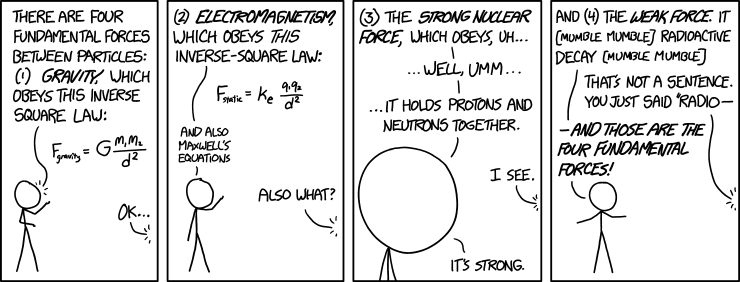
\includegraphics[scale=0.5]{fundamental_forces}

\begin{quote}
  \begin{itemize}
  \item[--]  Of these four forces, there's one we don't really understand.
  \item[--] Is it the weak force or the strong?
  \item[--]It's gravity.
  \end{itemize}
\end{quote}
\url{http://xkcd.com/1489/}

\section{Contenido de partículas}

\begin{frame}[fragile,allowframebreaks]
La materia conocida esta constituida de un cojunto de \emph{fermiones de Dirac} elementales definidos en la Tabla~\ref{tab:ef}
\begin{table}
  \centering
  \begin{tabular}{l|l|c|r}
    Tipo &Nombre & Simbolo&Carga\\\hline{}
   leptones& electrón & $e$& $-1$\\
          & neutrino & $\nu$ & $0$\\\hline{}
   quarks &quark up  & $u_1,u_2,u_3$ & $2/3$\\
          &quark down  & $d_1,d_2,d_3$& $-1/3$\\
  \end{tabular}
  \caption{Fermiones elementales:  The symbol represent both the particle, e.g $e^-$, as the antiparticle, e.g, $e^+$. The lectric chage is given in units of the electron chage $e$  }
  \label{tab:ef}
\end{table}
donde podemos definir los tripletes de color de quarks como
\begin{align}
  u=&
  \begin{pmatrix}
    u_1 \\ u_2\\ u_3\\
  \end{pmatrix}
  &d=&
  \begin{pmatrix}
    d_1 \\ d_2 \\ d_3\\
  \end{pmatrix}
\end{align}

Este conjunto de partículas esta bien definido para interacciones que conservan paridad como la interacción electromagnética o la fuerte. Para introducir la interacciones débiles usaremos más bien espinores de Weyl

\end{frame}

\section{Interacciones débiles}
\begin{frame}[fragile,allowframebreaks]
Las interacciones débiles son las responsables, entre otros fenoménos,
del decaimiento de neutrones libres en un protón, un electron y un
anti-neutrino electrónico. En nuestro entendimiento actual, se asume
que dicho decaimiento esta medidado por un bosón vectorial masivo y
cargado llamado $W^-_{\mu}$ con su correspondiente antipartícula
$W^{+}_{\mu}$. El caracter másivo da cuenta del corto alcance de la
interacción comparado con el rango infinito de la
interacción electromagnética mediada por un fotón sin masa
$A_{\mu}$. En la primera parte del decaimiento, el neutrón decae al
proton y un $W^{-}_{\mu}$ virtual, el cual a su vez decae en un
anti-neutrino derecho y un electrón izquierdo como se muestra en la
figura~\ref{fig:wnl}.

\begin{figure}
  \centering
  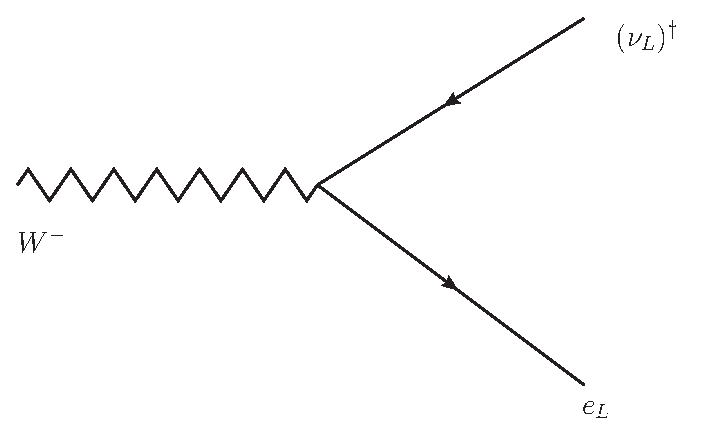
\includegraphics[scale=0.5]{wnl}
  \caption{Decaimiento del $W_\mu^-$.}
  \label{fig:wnl}
\end{figure}

Dicho decaimiento debe involucrar un término de interacción del tipo
\begin{align}
  \mathcal{L}_{W}\propto \left( \nu_L \right)^{\dagger}\overline{\sigma}^{\mu} e_L W_{\mu}^{+}.
\end{align}



Este tipo de interacción significa que en el contexto de las interacciones débiles un $e_L$ debe ser completamente
equivalente a un campo $\nu_L$. Es decir, el Lagrangiano debe ser
invariante bajo una transformación $\operatorname{SU}(2)_L$ de esos campos. A las energías normales, a las que se encuentra por ejemplo un neutrón dentro de un núcleo de Uranio, dicha simetría permanece oculta pues un electrón izquierdo y un neutrino izquierdo son campos completamente diferentes.
La
diferencia entre no sólo está en sus respectivas cargas eléctricas sino también
masas, pues la masa del neutrino es mucho más pequeña que la del electrón. 

Para poder explicar dicha interacción en el contexto de una simetría gauge local $\operatorname{SU}(2)_L$, debemos asumir que dicha simetría es explicita en alguna otra escala de energía donde en efecto  $e_L$ sea completamente
equivalente a $\nu_L$.

Debemos asumir entonces que ambos campos tienen una misma hipercarga,
asociada a una nueva simetría Abeliana $\operatorname{U}(1)_Y$ que sea la precursora de la simetría Abeliana de carga eléctrica $\operatorname{U}(1)_Q$. En tal caso, podríamos esperar que
la corriente electromagnética apropiada pueda obtenerse a partir del
Grupo semisimple $\operatorname{SU}(2)_L\times U(1)_Y$. Además. la respectiva masa para $W_{\mu}^{-}$
se podría obtener a partir del mecanismo de Higgs.

La simetría $\operatorname{SU}(2)_L$ entre las partes izquierdas del neutrino y el electrón, y entre las partes izquierdas de los quarks up y down, se establece  definiendo los dobletes:
  \begin{align}
    L\equiv\begin{pmatrix}
      \nu_L\\
      e_L      
    \end{pmatrix}\qquad   Q=&\begin{pmatrix}
    u_L\\
    d_L
  \end{pmatrix}\,,
  \end{align}
De otro lado, La invarianza bajo $U(1)_Y$ requiere que
\begin{align}
  Y_L=&Y_{\nu_L}=Y_{e_L}\nonumber\\
  Y_Q=&Y_{u_L}=Y_{d_L}\,.
\end{align}
El generador de carga eléctrica $\widehat{Q}$, se va obtener a partir de una combinación lineal del generador diagonal de $\operatorname{SU}(2)_L$, $T_3$, y del generador de hipercarga, $\widehat{Y}$.

Para considerar las interacciones débiles en conjunto con las interacciones electromágneticas y fuertes, es conveniente definir los campos de la primera generación en términos de los espinores ($\xi_{\alpha}$) y anti-espinores ($\eta^{\alpha}$) de Weyl izquierdos, de acuerdo a las convenciones de la Tabla~\ref{tab:electron}. El contenido de partículas con sus propiedades de transformación bajo el Grupo semisimple $\operatorname{SU}(3)_c\times \operatorname{SU}(2)_L\times U(1)_Y$ está dado en la Tabla~\ref{tab:fgw}, donde el $\mathbf{3}$ o el $\overline{\mathbf{3}}$ de $\operatorname{SU}(3)_c$ quieren decir que, además, para cada quark
\begin{align}
u_L=&
\begin{pmatrix}
  {u_{L}}_1\\
  {u_{L}}_2\\
  {u_{L}}_3
\end{pmatrix}&
  \left( u_R \right)^{\dagger}=&
  \begin{pmatrix}
    \left( u_R \right)^{\dagger}_1&
        \left( u_R \right)^{\dagger}_2&    \left( u_R \right)^{\dagger}_3
  \end{pmatrix},
\end{align}
etc.



\begin{table}
  \centering
  \begin{tabular}{l|c|c}\hline
    Nombre & Símbolo & $\left( \operatorname{SU}(3)_c, \operatorname{SU}(2)_L, U(1)_Y \right)$\\\hline
    $\Xi_{1\alpha}$: Doblete leptónico & $L=\displaystyle{\begin{pmatrix}
      \nu_L\\
      e_L      
    \end{pmatrix}}$ & $\left( \mathbf{1},\mathbf{2},Y_L \right)$\\
    $\Xi_{2\alpha}$: Doblete de quarks & $Q=\displaystyle{\begin{pmatrix}
      u_L\\
      d_L      
    \end{pmatrix}}$ & $\left( \mathbf{3},\mathbf{2},Y_Q \right)$\\
   $\eta^{\alpha}_1$: positrón izquierdo & $\left( e_R \right)^{\dagger}$&$\left(\mathbf{1},\mathbf{1},Y_{E}\right)$ \\
   $\eta^{\alpha}_2$: anti-up izquierdo & $\left( u_R \right)^{\dagger}$&$\left(\overline{\mathbf{3}},\mathbf{1},Y_{U}\right)$ \\
   $\eta^{\alpha}_3$: anti-down izquierdo & $\left( d_R \right)^{\dagger}$&$\left(\overline{\mathbf{3}},\mathbf{1},Y_{D}\right)$ \\
  \end{tabular}
  \caption{Spinores de Weyl izquierdos para la primera generación del modelo estándar}
  \label{tab:fgw}
\end{table}


Bajo la simetría $\operatorname{SU}(2)_L$, los campos transforman como:
 \begin{align}
  L\to L'=&\exp(i T^i \theta_i)L\approx(1+i T^i\theta_i)L\nonumber\\
  Q\to Q'=&\exp(i T^i \theta_i)Q\approx(1+i T^i\theta_i)Q\nonumber\\
  e_R\to& e'_R=e_R\nonumber\\
  u_R\to& u'_R=u_R\nonumber\\
  d_R\to& d'_R=d_R\,.
\end{align}
donde
\begin{align}
  T^i=\frac{\tau^i}{2}\,,
\end{align}
y $\tau^i$ son las matrices de Pauli dadas en la ec.~\eqref{eq:paulimatr}.

\end{frame}



\section{Simetría gauge local $\operatorname{SU}(3)_c\times  \operatorname{SU}(2)_L\times  U(1)_Y$}
\begin{frame}[fragile,allowframebreaks]
Los términos de masa de Dirac, usando las convenciones de la
Tabla~\ref{tab:fgw} no son invariantes bajo la simetría $\operatorname{SU}(2)_L$ porque
no hay forma de escribir términos escalares usando combinaciones los
campos $\Xi$ y $\eta$.  De la ec.~\eqref{eq:dwlag}, y usando la definición para los dobletes adjuntos de $\operatorname{SU}(2)_L$ en la ec.~\eqref{eq:Xiadj}, el Lagrangiano más
general posible para los campos de la Tabla~\ref{tab:fgw} compatibles
con las simetría de Lorentz y el grupo global $\operatorname{SU}(3)_c\times
\operatorname{SU}(2)_L\times U(1)_Y$ es
\begin{align}
  \mathcal{L}=&\sum_{i=1}^2i\epsilon_{ab}\widetilde{\Xi}_i^{a}\overline{\sigma}^{\mu}\partial_{\mu}\Xi_i^{b}
+\sum_{i=1}^3i\eta_{i}\sigma^{\mu}\partial_{\mu} \eta^{\dagger}_i\nonumber\\
  =&\sum_{i=1}^2i\widetilde{\Xi}_i\cdot\overline{\sigma}^{\mu}\partial_{\mu}\Xi_i
+\sum_{i=1}^3i\eta_{i}\sigma^{\mu}\partial_{\mu} \eta^{\dagger}_i\nonumber\\
=&i\widetilde{L}\cdot\overline{\sigma}^{\mu}\partial_{\mu}L+i\widetilde{Q}\cdot\overline{\sigma}^{\mu}\partial_{\mu}Q
+i(e_R)^{\dagger}\sigma^{\mu}\partial_{\mu} e_R+i(u_R)^{\dagger}\sigma^{\mu}\partial_{\mu} u_R+i
(d_R)^{\dagger}\sigma^{\mu}\partial_{\mu} d_R \nonumber\\
=&i(\nu_L)^{\dagger}\overline{\sigma}^{\mu}\partial_{\mu}\nu_L+i(e_L)^{\dagger}\overline{\sigma}^{\mu}\partial_{\mu}e_L
+i (u_L)^{\dagger}\overline{\sigma}^{\mu}\partial_{\mu}u_L+i(d_L)^{\dagger}\overline{\sigma}^{\mu}\partial_{\mu}d_L \nonumber\\
&+i(e_R)^{\dagger}\sigma^{\mu}\partial_{\mu}e_R+i(u_R)^{\dagger}\sigma^{\mu}\partial_{\mu} u_R+i(d_R)^{\dagger}\sigma^{\mu}\partial_{\mu} d_R \,,
\end{align}
donde
\begin{align}
\label{eq:widetildeLQ}
  \widetilde{L}=&
  \begin{pmatrix}
   \left(e_L\right)^{\dagger}\\
  - \left(\nu_L  \right)^{\dagger}\\
  \end{pmatrix},&
  \widetilde{Q}=&
  \begin{pmatrix}
   \left(d_L\right)^{\dagger}\\
  - \left(u_L  \right)^{\dagger}\\
  \end{pmatrix},&
\end{align}
de modo que
\begin{align*}
  i\widetilde{L}\cdot\overline{\sigma}^{\mu}\partial_{\mu}L=&
  i\,\epsilon_{ab}\widetilde{L}\cdot\overline{\sigma}^{\mu}\partial_{\mu}L \nonumber\\
 =&i\,\widetilde{L}^1\overline{\sigma}^{\mu}\partial_{\mu}L^2-i\,\left( -\widetilde{L}^2 \right)\overline{\sigma}^{\mu}\partial_{\mu}L^1    \nonumber\\
 =&i\,\left( e_L \right)^{\dagger}\overline{\sigma}^{\mu}\partial_{\mu}e_L+i\,\left( \nu_L \right)^{\dagger}\overline{\sigma}^{\mu}\partial_{\mu}\nu_L    \nonumber\\
\end{align*}
y lo mismo para $Q$.



Para obtener la interacciones del modelo estándar, reemplazamos las derivadas normales por derivadas covariantes.

Proponemos entonces el Lagrangiano
\begin{align}
\label{eq:L0}
     \mathcal{L}=&i\widetilde{Q}\cdot \overline{\sigma}^\mu\mathcal{D}_\mu Q+i\widetilde{L}\cdot \overline{\sigma}^\mu\mathcal{D}_\mu L+
i(e_R)^{\dagger}\sigma^\mu\mathcal{D}_\mu {e_R}+i(d_R)^{\dagger}\sigma^\mu\mathcal{D}_\mu d_R+i(u_R)^{\dagger}\sigma^\mu\mathcal{D}_\mu {u_R}
\nonumber\\
     &-\tfrac{1}{4}G^{\mu\nu}_a G_{\mu\nu}^a-\tfrac{1}{4}W^{\mu\nu}_i W_{\mu\nu}^i-\tfrac{1}{4}B^{\mu\nu} B_{\mu\nu}\,,
\end{align}
donde
\begin{align}
  \mathcal{D}^\mu&\equiv\partial^\mu-i g_s\frac{\lambda^a}{2}G^\mu_a-i g \frac{\tau^i}{2}W^\mu_i-i {g_1}YB^\mu\,.
\end{align}
y además
\begin{align*}
  \Lambda^a\equiv\frac{\lambda^a}{2},\ a=1,2,\ldots,8 &\qquad\text{8 generadores de $\operatorname{SU}(3)_c$}\\
  T^i\equiv\frac{\tau^i}{2},\ i=1,2,3 &\qquad\text{3 generadores de $\operatorname{SU}(2)_L$}\\
  Y &\qquad\text{generador de $U(1)_Y$},
\end{align*}
A este nivel, tanto los 15 fermiones de Weyl (cada quark izquierdo y derecho viene en tres colores), como los 12 bosones gauge, \emph{tienen masa nula}. Necesitamos entonces un mecanismo de ruptura espontánea de simetría para generar por lo menos masas para los tres bosones gauge asociados a la interacción débil, el cual será abordado en la Sección~\ref{sec:rupt-espont-de}.



\end{frame}
Además,
\begin{align}
  W_{\mu \nu}^i=&\partial_\mu W_\nu^i -\partial_\mu W_\mu^i+ g \epsilon_{ijk}W_\mu^j W_\nu^k \nonumber\\
  B_{\mu \nu}=&\partial_\mu B_\nu -\partial_\mu B_\mu\,.
\end{align}
y $G_{\mu\nu}^a$ está dado en la ec.~\eqref{eq:258qft}.

Bajo una transformación gauge local, las derivadas covariantes de los campos (y por consiguiente los campos) transforman como:
\begin{align}
  \mathcal{D}_\mu L&\to\left(\mathcal{D}_\mu L\right)'=\exp\left(-i\theta_iT^i-i\beta Y_L\right)\mathcal{D}_\mu L\nonumber\\
  \mathcal{D}_\mu Q&\to\left(\mathcal{D}_\mu Q\right)'=\exp\left(-i\alpha_a\Lambda^a-i\theta_iT^i-i\beta Y_Q\right)\mathcal{D}_\mu Q\nonumber\\
  \mathcal{D}_\mu \Phi&\to\left(\mathcal{D}_\mu \Phi\right)'=\exp\left(-i\theta_iT^i-i\beta Y_\Phi\right)\mathcal{D}_\mu \Phi\nonumber\\
  \mathcal{D}_\mu e_R&\to\left(\mathcal{D}_\mu e_R\right)'=\exp\left(-i\beta Y_{E}\right)\mathcal{D}_\mu e_R=\exp\left(-i\beta Q_{e}\right)\mathcal{D}_\mu e_R\nonumber\\
  \mathcal{D}_\mu d_R&\to\left(\mathcal{D}_\mu d_R\right)'=\exp\left(-i\alpha_a\Lambda^a-i\beta Y_{D}\right)\mathcal{D}_\mu d_R=\exp\left(-i\alpha_a\Lambda^a-i\beta Q_{d}\right)\mathcal{D}_\mu d_R\nonumber\\
  \mathcal{D}_\mu u_R&\to\left(\mathcal{D}_\mu u_R\right)'=\exp\left(-i\alpha_a\Lambda^a-i\beta Y_{U}\right)\mathcal{D}_\mu u_R=\exp\left(-i\alpha_a\Lambda^a-i\beta Q_{u}\right)\mathcal{D}_\mu u_R\,.
\end{align}
donde $Q_{e}=-1$, etc, son las cargas eléctricas asociadas a los campos.


\section{Ruptura espontánea de simetría}
\label{sec:rupt-espont-de}

\begin{frame}[fragile,allowframebreaks]
Todas las partículas en este lagrangiano son no masivas. Esto funciona sólo para los gluones y uno de los bosones gauge abelianos, pero no es realista para los bosones gauge cargados. 
Para solucionar este problema se postula la existencia de un nuevo doblete escalar complejo
( y su correspondiente adjunto de $\operatorname{SU}(2)$) con cuatro grados de libertad:
\begin{align}
\label{eq:Phi}
  \Phi=&
  \begin{pmatrix}
    \phi^+\\
    \phi^0\\
  \end{pmatrix}=
  \begin{pmatrix}
    \phi_1+i\phi_2\\
\phi_3+i\phi_4
  \end{pmatrix},&
\widetilde{\Phi}=&
  \begin{pmatrix}
    \left( \phi^0 \right)^{*}\\
   -\phi^-\\
  \end{pmatrix}\,.
\end{align}
El  ``$\pm$'' y el superíndice 0, se ponen de forma conveniente para obtener expresiones consitentes. Es claro que $\left( \phi^+ \right)^{*}=\phi^-\,.$





Es posible ahora construir invariantes $\operatorname{SU}(2)$ con las siguientes combinaciones de campos similares al del término de masa de Dirac en~\eqref{eq:dwlag}
\begin{align}
 -\eta_1\,\Xi_1\cdot\widetilde{\Phi}-\left(\eta_1\,\Xi_1\cdot\widetilde{\Phi}  \right)^{\dagger}
 =& -\eta_1\,\Xi_1\cdot\widetilde{\Phi}-\text{h.c}\nonumber\\
 =& -\eta^{b}_1\,\epsilon_{ab}\,\Xi_1^{a}\cdot\widetilde{\Phi}^{b}-\text{h.c} \nonumber\\
   =&-\left( e_R \right)^{\dagger}\epsilon_{ab}L^a\widetilde{\Phi}^b -\text{h.c} \nonumber\\
   =&\left( e_R \right)^{\dagger}L^1\widetilde{\Phi}^2+\left( e_R \right)^{\dagger}L^1\widetilde{\Phi}^2 +\text{h.c} \nonumber\\
   =&\left( e_R^{-} \right)^{\dagger}\nu_L\phi^- +\left( e_R^{-} \right)^{\dagger}e_L^-\phi^0 +\text{h.c} \,,
 \end{align}
donde $\text{h.c}$, denota el hermítico conjugado de cada término (para garantizar que el Lagrangiano sea real)
y hemos puesto la carga del electrón para hacer explícita la conservación de la carga eléctrica. 

Note que
\begin{align}
  \left( e_R \right)^{\dagger}\epsilon_{ab}L^a\widetilde{\Phi}^b=\left( e_R \right)^{\dagger}L\cdot \widetilde{\Phi}\,.
\end{align}


\end{frame}
\begin{frame}[fragile,allowframebreaks]
El Lagrangiano completo involucrando estos campos es
\begin{align}
     \mathcal{L}=&i\widetilde{Q}\cdot \overline{\sigma}^\mu\mathcal{D}_\mu Q+i\widetilde{L}\cdot \overline{\sigma}^\mu\mathcal{D}_\mu L+
i(e_R)^{\dagger}\sigma^\mu\mathcal{D}_\mu {e_R}+i(d_R)^{\dagger}\sigma^\mu\mathcal{D}_\mu {d_R}+i(u_R)^{\dagger}\sigma^\mu\mathcal{D}_\mu {u_R}
\nonumber\\
     &-\tfrac{1}{4}G^{\mu\nu}_a G_{\mu\nu}^a-\tfrac{1}{4}W^{\mu\nu}_i W_{\mu\nu}^i-\tfrac{1}{4}B^{\mu\nu} B_{\mu\nu}\nonumber\\
     &+\widetilde{\left( \mathcal{D}_\mu{\Phi} \right)}\cdot\mathcal{D}^\mu\Phi-\mu^2\widetilde{\Phi}\cdot\Phi-\lambda \left( \widetilde{\Phi}\cdot\Phi \right)^2\nonumber\\
     &- \left[  h_e \left( e_R \right)^{\dagger}\,L\cdot \widetilde{\Phi}_b +
      h_d \left( d_R \right)^{\dagger}\,Q\cdot \widetilde{\Phi} +
      h_u \left( u_R \right)^{\dagger}\,Q\cdot {\Phi}+\text{h.c}\right]\nonumber\\
     =&\mathcal{L}_{\text{fermion}}+\mathcal{L}_{\text{gauge}}
     +\mathcal{L}_{WBH}
     -\mathcal{L}_{\text{Yukawa}}\,.
\end{align}
donde $\mu^2<0$, y $\lambda>0$,
\begin{align}
  \widetilde{\Phi}=&i\tau_2\Phi^* 
% \nonumber\\
% =&i
% \begin{pmatrix}
%   0 & -i \\
%  i & 0\\
% \end{pmatrix}
% \begin{pmatrix}
%   \phi^+\\
% \phi^0
% \end{pmatrix}^{*} \nonumber\\
% =&\begin{pmatrix}
%   0 & 1 \\
%  -1 & 0\\
% \end{pmatrix}
% \begin{pmatrix}
%   \phi^-\\
% {\phi^0}^{*}
%\end{pmatrix} \nonumber\\
=\begin{pmatrix}
{\phi^0}^{*}\\
-  \phi^-\\
\end{pmatrix}, &   \Phi=&
  \begin{pmatrix}
    \phi^+\\
    \phi^0\\
  \end{pmatrix}.
\end{align}

\end{frame}
\begin{frame}[fragile,allowframebreaks]
Resumiendo

\begin{align}
  \label{eq:smscalar}
\mathcal{L}_{\text{fermion}}=&i\widetilde{Q}\cdot \overline{\sigma}^\mu\mathcal{D}_\mu Q+i\widetilde{L}\cdot \overline{\sigma}^\mu\mathcal{D}_\mu L \nonumber\\
&+i(e_R)^{\dagger}\sigma^\mu\mathcal{D}_\mu {e_R}+i(d_R)^{\dagger}\sigma^\mu\mathcal{D}_\mu {d_R}+i(u_R)^{\dagger}\sigma^\mu\mathcal{D}_\mu {u_R}\nonumber\\
  \mathcal{L}_{WBH}=&\widetilde{\left( \mathcal{D}_\mu{\Phi} \right)}\cdot\mathcal{D}^\mu\Phi-\mu^2\widetilde{\Phi}\cdot\Phi-\lambda \left( \widetilde{\Phi}\cdot\Phi \right)^2 \nonumber\\
\mathcal{L}_{\text{gauge}}=& -\tfrac{1}{4}G^{\mu\nu}_a G_{\mu\nu}^a-\tfrac{1}{4}W^{\mu\nu}_i W_{\mu\nu}^i-\tfrac{1}{4}B^{\mu\nu} B_{\mu\nu}\nonumber\\
  % =&(\mathcal{D}_\mu\Phi)^\dagger\mathcal{D}^\mu\Phi-\mu^2\Phi^\dagger\Phi-\lambda(\Phi^\dagger\Phi)^2\nonumber\\
%=&(\mathcal{D}_\mu\widetilde{\Phi})^\dagger\mathcal{D}^\mu\widetilde{\Phi}-\mu^2\widetilde{\Phi}^\dagger\widetilde{\Phi}-\lambda(\widetilde{\Phi}^\dagger\widetilde{\Phi})^2\nonumber\\
-\mathcal{L}_{\text{Yukawa}}=&  h_e \left( e_R \right)^{\dagger}\,L\cdot \widetilde{\Phi}_b +
      h_d \left( d_R \right)^{\dagger}\,Q\cdot \widetilde{\Phi} +
      h_u \left( u_R \right)^{\dagger}\,Q\cdot {\Phi}+\text{h.c}
\end{align}
Para el potencial escalar usaremos la forma más conveniente del producto matricial para el invariante de $\operatorname{SU}(2)_L$ por que no hay ambigüedad con el conjugado de un campo escalar.

Para los campos del Lagrangiano, debemos asegurarnos de que todos los términos invariantes gauge locales y renormalizables sean considerados. De hecho, términos de interacción entre fermiones y el campo escalar, correspondiente a una interacción de Yukawa, son invariantes bajo transformaciones $SU(3)_c\times  SU(2)_L\times  U(1)_Y$ si
\end{frame}
\begin{frame}[fragile,allowframebreaks]
\begin{align*}
  Y_L+Y_{\widetilde{\Phi}}-Q_{e}=&0\\
  Y_Q+Y_{\widetilde{\Phi}}-Q_{d}=&0\\
  Y_Q+Y_{\Phi}-Y_{u}=Y_Q-Y_{\widetilde{\Phi}}-Q_{u}=&0\,,
\end{align*}
donde hemos fijado $Y_{\widetilde{\Phi}}=-Y_\Phi$. Solucionado para las hipercargas de los dobletes tenemos
\begin{align}
\label{eq:yyy}
Y_L=&\frac{1}{2}\left( -Q_d+2Q_e+Q_u \right)=-\frac{1}{2}  \nonumber\\
Y_Q=&\frac{1}{2}\left( Q_d+Q_u \right)=\frac{1}{6} \nonumber\\
Y_{\widetilde{\Phi}}=-Y_{\Phi}=&\frac{1}{2}\left( Q_d-Q_u \right)=-\frac{1}{2}\,.
\end{align}

De este modo, es consistente interpretar los superíndices de $\phi^+$ y $\phi^0$ en la ec.~\eqref{eq:Phi} como las cargas eléctricas de las componentes del doblete de Higgs, $\Phi$.

\end{frame}

El potencial escalar contiene los términos
\begin{align}
  V(\Phi)=\mu^2\widetilde{\Phi}\cdot\Phi+\lambda \left( \widetilde{\Phi}\cdot\Phi \right)^2 
\end{align}
con $\mu^2<0$ y $\lambda>0$. % se reduce a
% \begin{align}
%   V(H)=\frac{1}{2}\mu^2(H+v)^2+\frac{1}{4}\lambda (H+v)^4\,.
% \end{align}


El modelo estándar es entonces una combinación de una teoría gauge local $\operatorname{SU}(3)_{c}$ con una simetría gauge local con ruptura espontánea de simetría (RES) $\operatorname{SU}(2)_L\times \operatorname{U}(1)_Y$. A continuación nos enfocaremos de momento en la parte leptónica de  $\operatorname{SU}(2)_L\times \operatorname{U}(1)_Y$ con RES.

\section{Una teoría para leptones de la primera generación}
\begin{frame}[fragile,allowframebreaks]
Comenzaremos analizando una versión simplificada del Lagrangiano con sólo los leptones de la primera de generación,
\begin{align}
  \mathcal{L}^{\text{lepton}}=\mathcal{L}_{\text{fermion}}^{\text{lepton}}+
   \mathcal{L}_{WBH}+\mathcal{L}_{\text{gauge}}-\mathcal{L}_{\text{Yukawa}}^{\text{lepton}}\,,
\end{align}
donde
\begin{align}
  \label{eq:smscalarlep}
\mathcal{L}_{\text{fermion}}^{\text{lepton}}=&i\widetilde{L}\cdot \overline{\sigma}^\mu\mathcal{D}_\mu L 
+i(e_R)^{\dagger}\sigma^\mu\mathcal{D}_\mu {e_R}\nonumber\\
  \mathcal{L}_{WBH}=&\widetilde{\left( \mathcal{D}_\mu{\Phi} \right)}\cdot\mathcal{D}^\mu\Phi-\mu^2\widetilde{\Phi}\cdot\Phi-\lambda \left( \widetilde{\Phi}\cdot\Phi \right)^2 \nonumber\\
\mathcal{L}_{\text{gauge}}=& -\tfrac{1}{4}W^{\mu\nu}_i W_{\mu\nu}^i-\tfrac{1}{4}B^{\mu\nu} B_{\mu\nu}\nonumber\\
  % =&(\mathcal{D}_\mu\Phi)^\dagger\mathcal{D}^\mu\Phi-\mu^2\Phi^\dagger\Phi-\lambda(\Phi^\dagger\Phi)^2\nonumber\\
%=&(\mathcal{D}_\mu\widetilde{\Phi})^\dagger\mathcal{D}^\mu\widetilde{\Phi}-\mu^2\widetilde{\Phi}^\dagger\widetilde{\Phi}-\lambda(\widetilde{\Phi}^\dagger\widetilde{\Phi})^2\nonumber\\
-\mathcal{L}_{\text{Yukawa}}^{\text{lepton}}=&  h_e \left( e_R \right)^{\dagger}\,L\cdot \widetilde{\Phi}_b +\text{h.c}
\end{align}
y sin perdida de generalidad para las partes del Lagrangiano $\mathcal{L}_{\text{gauge}}$ y $ \mathcal{L}_{WBH}\,$ que no involucran fermiones.
\end{frame}

\subsection{Interacciónes débiles fermión-gauge para leptones}

Nos enfocaremos de momento en la parte leptónica pues las interacciones para quarks involucran el mismo tipo de cálculos.

Los términos de interacción generados por la simetría gauge para el sector leptónico son:
\begin{align}
\label{eq:devLW}
 \mathcal{L}_{\text{fermion}}^{\text{lepton}}=& i \widetilde{L}\cdot\overline{\sigma}^\mu\mathcal{D}_\mu L+  i \left( e_R \right)^{\dagger}{\sigma}^\mu\mathcal{D}_\mu e_R \nonumber\\
=&i \widetilde{L}\cdot\overline{\sigma}^\mu\partial_\mu L+i \left(e_R  \right)^{\dagger}\sigma^\mu\partial_\mu {e_R} \nonumber\\
&+ i \widetilde{L}\cdot\overline{\sigma}^\mu(-i g_2 T_iW_\mu^i-i {g_1}\,Y_LB_\mu) L + i \left( e_R \right)^{\dagger}\sigma^\mu \left( -i{g_1} Y_R B_{\mu} \right) {e_R}\,.
\end{align}
Definiendo
\begin{align}
\label{eq:knt}
  \mathcal{L}_{\text{kinetic}}=&i \widetilde{L}\cdot\overline{\sigma}^\mu\partial_\mu L+i \left(e_R  \right)^{\dagger}\sigma^\mu\partial_\mu {e_R} \\
  \mathcal{L}_{WBL}=&i \widetilde{L}\cdot\overline{\sigma}^\mu(-i g_2 T_iW_\mu^i-i {g_1}\,Y_LB_\mu) L + i \left( e_R \right)^{\dagger}\sigma^\mu \left( -i{g_1} Y_R B_{\mu} \right) {e_R}\nonumber\,.
\end{align}
tenemos que
\begin{align}
\mathcal{L}_{WBL}=& \widetilde{L}\cdot\overline{\sigma}^\mu(g_2 T_1W_\mu^1+ g_2 T_2W_\mu^2+g_2 T_3W_\mu^3+{g_1}\,Y_LB_\mu) L+ g_1 Y_R\left(e_R \right)^{\dagger}\sigma^\mu  {e_R} B_\mu\nonumber\\
=& \widetilde{L}\cdot\overline{\sigma}^\mu\left[\frac{g_2}{\sqrt{2}}
  \begin{pmatrix}
0 & W_\mu^+\\
W_\mu^- & 0\\    
  \end{pmatrix}
+g_2 T_3W_\mu^3+{g_1}\,Y_LB_\mu
\right]L+ {g_1} Y_R\left(e_R \right)^{\dagger}\sigma^\mu  {e_R} B_\mu\nonumber\\
=&i \widetilde{L}\cdot\overline{\sigma}^\mu\frac{g_2}{\sqrt{2}}
  \begin{pmatrix}
0 & W_\mu^+\\
W_\mu^- & 0\\    
  \end{pmatrix}L+
 \widetilde{L}\cdot\overline{\sigma}^\mu\left[g_2 T_3W_\mu^3+{g_1}\,Y_LB_\mu
\right]L+ {g_1} Y_R\left(e_R \right)^{\dagger}\sigma^\mu  {e_R} B_\mu\nonumber\\
  =& \frac{g_2}{\sqrt{2}}\widetilde{L}\cdot\overline{\sigma}^\mu
  \begin{pmatrix}
e_LW_\mu^+\\
\nu_L W_\mu^-\\    
  \end{pmatrix}+\mathcal{L}_{A Z L}\,,
\end{align}

donde
\begin{align}
\label{eq:lazl}
  \mathcal{L}_{A Z L}=& \widetilde{L}\cdot\overline{\sigma}^\mu\left[g_2 T_3W_\mu^3+{g_1}\,Y_LB_\mu\right]L+ {g_1} Y_R\left(e_R \right)^{\dagger}\sigma^\mu  {e_R} B_\mu\,.
\end{align}

Teniendo en cuenta que 
\begin{align}
  \frac{g_2}{\sqrt{2}}\widetilde{L}\cdot\overline{\sigma}^\mu
  \begin{pmatrix}
e_LW_\mu^+\\
\nu_L W_\mu^-\\    
  \end{pmatrix}=\frac{g_2}{\sqrt{2}} \left[ \epsilon^{12} \widetilde{L}_1 \overline{\sigma}^{\mu} \nu_L W_{\mu}^-
+\epsilon^{21}  \widetilde{L}_2 \overline{\sigma}^{\mu} e_L W_{\mu}^+ \right],
\end{align}
y usando \eqref{eq:widetildeLQ}
\begin{align}
  \frac{g_2}{\sqrt{2}}\widetilde{L}\cdot\overline{\sigma}^\mu
  \begin{pmatrix}
e_LW_\mu^+\\
\nu_L W_\mu^-\\    
  \end{pmatrix}=\frac{g_2}{\sqrt{2}} \left[\left( e_L \right)^{\dagger} \overline{\sigma}^{\mu} \nu_L W_{\mu}^-
+ \left( \nu_L \right)^{\dagger} \overline{\sigma}^{\mu} e_L W_{\mu}^+ \right].
\end{align}
De este modo, la simetría gauge genera la interacción deseada con los bosones gauge cargados $W_{\mu}^{\pm}$. Sin embargo, se generan muchas otras interacciones las cuales deben contener apropiadamente la interacción electromagnética en algún cambio de base.

% Reemplazando en \eqref{eq:devLW}
% \begin{align}
%     i \widetilde{L}\cdot\overline{\sigma}^\mu\mathcal{D}_\mu L-i \widetilde{L}\cdot\overline{\sigma}^\mu\partial_\mu L
%   =&
% \frac{g_2}{\sqrt{2}}\left[\left( \nu_L \right)^{\dagger}\overline{\sigma}^\mu e_LW_\mu^++
% \left( e_L \right)^{\dagger}\overline{\sigma}^\mu\nu_L W_\mu^-\right]    
% +\mathcal{L}_{A Z L}\nonumber\\
%   =&
% \mathcal{L}_{W L}    
% +\mathcal{L}_{A Z L}\,,
% \end{align}
Entonces
\begin{align}
  \mathcal{L}_{WBL}= \mathcal{L}_{W L}+  \mathcal{L}_{A Z L}\,,
\end{align}
donde
\begin{align}
\label{eq:lwl}
  \mathcal{L}_{W L}=&\frac{g_2}{\sqrt{2}}\left[\left( \nu_L \right)^{\dagger}\overline{\sigma}^\mu e_LW_\mu^++
\left( e_L \right)^{\dagger}\overline{\sigma}^\mu\nu_L W_\mu^-\right].
\end{align}

El principal problema con $\mathcal{L}_{AZL}$ en la ec.~\eqref{eq:lazl} es que el neutrino izquierdo $\nu_L$ presente en $L$ se acopla a los dos bosones gauge neutros $W_3^{\mu}$ y $B^{\mu}$. Debemos buscar una base en la cual se pueda recuperar la interacción electromagnética de tal forma que el fotón $A_{\mu}$ no se acople a partículas neutras como el neutrino, $\nu_L$. Definimos entonces el posible fotón a partir de la rotación
\begin{equation}
\label{eq:rottw}
  \begin{pmatrix}
    W_3^\mu\\
    B^\mu
  \end{pmatrix}=\begin{pmatrix}
    \cos\theta_W & \sin\theta_W\\
    -\sin\theta_W& \cos\theta_W
  \end{pmatrix}
  \begin{pmatrix}
    Z^\mu\\
    A^\mu
  \end{pmatrix}.
\end{equation}
donde $\theta_{W}$, es el ángulo de rotación débil (Weak de sus siglas en inglés) y $Z^{\mu}$ es el otro campo que resulta de la rotación a la nueva base que define al fotón $A^{\mu}$.
Aplicando esta rotación a~\eqref{eq:lazl}, tenemos que
\begin{align}
\label{eq:brot}
   \mathcal{L}_{A Z L}=& \widetilde{L}\cdot\overline{\sigma}^\mu\left[g_2 T_3(c_W Z_\mu+s_W A_\mu)+{g_1}\,Y_L(-s_W Z_\mu+c_W A_\mu)\right]L
    +g_1 Y_R\left(e_R \right)^{\dagger}\sigma^\mu  {e_R} (-s_W Z_\mu+c_W A_\mu)\nonumber\\
     =& \widetilde{L}\cdot\overline{\sigma}^\mu\left[g_2 T_3c_W Z_\mu+g_2 T_3s_W A_\mu-{g_1}\,Y_Ls_W Z_\mu+{g_1}\,Y_Lc_W A_\mu\right]L\nonumber\\
&-g_1 s_W Y_R\left(e_R \right)^{\dagger}\sigma^\mu  {e_R}Z_{\mu}  +g_1 c_W Y_R\left(e_R \right)^{\dagger}\sigma^\mu  {e_R}A_{\mu}  \nonumber\\
    =& \widetilde{L}\cdot\overline{\sigma}^\mu\left[\left(g_2 c_WT_3-{g_1}s_W\,Y_L\right)Z_\mu
       +\left(g_2 s_W T_3+{g_1}c_W\,Y_L\right) A_\mu\right]L \nonumber\\
&-g_1 s_W Y_R\left(e_R \right)^{\dagger}\sigma^\mu  {e_R}Z_{\mu}  +g_1 c_W Y_R\left(e_R \right)^{\dagger}\sigma^\mu  {e_R}A_{\mu}  \,,
\end{align}
donde $c_W=\cos\theta_W$, $s_W=\sin\theta_W$. 

Para identificar $A_{\mu}$ con el fotón, debemos imponer la condición
\begin{align}
  \label{eq:relgn}
e\widehat{Q}=g_2 s_W T_3+{g_1}c_W\,\widehat{Y}\,.
\end{align}
De este modo
\begin{align}
  e\widehat{Q}L =& \left(g_2 s_W T_3+{g_1}c_W\,\widehat{Y}\right) L \nonumber\\
=& \left(g_2 s_W T_3+{g_1}c_W\,Y_L\right) L \,,
\end{align}
Usando la definición de $L$ tenemos que
\begin{align}
 e
  \begin{pmatrix}
    Q_{\nu} \nu_L\\
       Q_e e_L 
 \end{pmatrix}=
    e\begin{pmatrix}
   0\\
      Q_e e_L \\
  \end{pmatrix}=
  \begin{pmatrix}
   \left( \frac{1}{2}g_2 s_W +g_1 c_W Y_L \right) \nu_L\\ 
 \left(  -\frac{1}{2}g_2 s_W +g_1 c_W Y_L \right) e_L
  \end{pmatrix}
\end{align}
Igualando los coeficientes que acompañan los campos resultan las dos condiciones
\begin{align}
  \label{eq:g2sw}
  0= & \frac{1}{2}g_2 s_W +g_1 c_W Y_L  \\
    \label{eq:YL}
e Q_e=& \left(  -\frac{1}{2}g_2 s_W +g_1 c_W Y_L \right)
\end{align}
una tercera condición surge de imponer que el electrón derecho se acople apropiadamente al fotón
\begin{align}
  \label{eq:erel}
 e\widehat{Q} e_R =& \left(g_2 s_W T_3+{g_1}c_W\,\widehat{Y}\right) e_R\nonumber\\  
e Q_e e_R=& g_1 c_W\,Y_R \, e_R\,.
\end{align}
con estas condiciones podemos despejar tres incógnitas que corresponden a $g_1c_W$, $g_2s_W$ y $Y_L$.
La primera de ellas la podemos obtener de 
igualar los coeficientes que acompañan los campos para la tercera condición, teniendo en cuenta que $\widehat{Q}=\widehat{Y}$ para los campos derechos los cuales no participan de la interacción
débil asociada a $\operatorname{SU}(2)_L$
\begin{align}
  e=g_1 c_W\,.
\end{align}
Reemplazando en \eqref{eq:g2sw}
\begin{align}
  g_2 s_W = -2e Y_L\,,
\end{align}
y reemplazando ambos resultado en \eqref{eq:YL}, obtenemos
\begin{align}
  eQ_e=-\frac{1}{2} e+eY_L\,,
\end{align}
de donde podemos despejar $Y_L$ 
\begin{align}
  Y_L=Q_e+\frac{1}{2}=-1+\frac{1}{2}=-\frac{1}{2}\,.
\end{align}

El resultado final es entonces
\begin{align}
\label{eq:esc}
 Y_L=&-\frac{1}{2}\,,&   e=&g_2\sin\theta_W=g_1 \cos\theta_W\,.
\end{align}
La segunda ecuación se puede usara en la ec.~\eqref{eq:relgn} para obtener la predicción en término de los generadores diagonales válida para cualquier campo fermiónico
\begin{align}
\label{eq:gn}
 \widehat{Q}=&T_3+\widehat{Y}\,.
\end{align}

La ec. \eqref{eq:gn}, se conoce como la relación de Gell-Mann--Nishijima, y junto con~\eqref{eq:esc}, establece las condiciones que se deben satisfacer para obtener apropiadamente la QED a partir de la interacción electrodébil asociada al grupo semisimple $\operatorname{SU}(2)_L\times  U(1)_Y$.

\noindent
\textbf{Ejercicio}: Demostrar que los valores numéricos de las hipercargas en \eqref{eq:yyy} son consistentes con la relación de Gell-Mann--Nishijima \eqref{eq:gn}:
\begin{align}
 \widehat{Q}=&T_3+\widehat{Y}\,.
\end{align}


De la segunda ecuación  \eqref{eq:esc}, podemos expresar el ángulo $\theta_W$ en términos de $g_1$ y $g_2$ como
\begin{align}
\label{eq:twa}
  \tan\theta_W=\frac{g_1}{g_2}\,.
\end{align}

A modo de ilustración podemos comprobar
los valores numéricos para $Y_L$ y $Y_R$ usando directamente la relación de Gell-Mann--Nishijima \eqref{eq:gn}
\begin{align}
  \widehat{Q}L=&(T_3+Y_L)L \nonumber\\
  \begin{pmatrix}
    Q_\nu & 0\\
    0  & Q_e
  \end{pmatrix}
  \begin{pmatrix}
    \nu_L\\
    e_L
  \end{pmatrix}=  
  \begin{pmatrix}
   Q_{\nu} \nu_L\\
   Q_e e_L
  \end{pmatrix}
= & \begin{pmatrix}
    \frac{1}{2} + Y_L & 0\\
    0  & -\frac{1}{2}+Y_L
  \end{pmatrix}  \begin{pmatrix}
    \nu_L\\
    e_L
  \end{pmatrix} \,,
\end{align}
de modo que
\begin{align}
  Q_{\nu}&=0=\frac{1}{2}+Y_L\,, & Q_e&=-1=-\frac{1}{2}+Y_L\,,
\end{align}
lo cual  requiere que
\begin{align}
  Y_L=\frac{1}{2}\,.
\end{align}
De la misma forma
\begin{align}
  Y_R=Q_e=-1\,.
\end{align}
Note que para campos derechos la hipercarga coincide con la carga eléctrica.


Usando la relación entre $g_2$ y ${g_1}$~\eqref{eq:twa} en ~\eqref{eq:brot}
\begin{align}
    \mathcal{L}_{A Z L}
=&g_2 s_W \widetilde{L}\cdot\overline{\sigma}^\mu\left[\left(\cot\theta_WT_3- \tan\theta_W\,Y_L\right)Z_\mu
       +\left(T_3+Y_L\right) A_\mu\right]L \nonumber\\
&+g_2 s_W \left(e_R \right)^{\dagger}\sigma^\mu \left[ \left(0 -\tan\theta_W  Y_R  \right) Z_{\mu}  +\left( 0+ Y_R \right)  A_{\mu} \right]{e_R}\,,
\end{align}
donde hemos puesto explícitamente el cero correspondiente a: $T_3 e_R= 0 \,e_R$.

Como el generador asociado a $A_\mu$ debe ser el generador de carga eléctrica, podemos usar la primera ecuación en~\eqref{eq:esc}:
\begin{align}
  e=g_2\sin\theta_W\,,
\end{align}
y si además definimos
\begin{align}
  \mathcal{L}_{E}=g_2 s_W \left(e_R \right)^{\dagger}\sigma^\mu \left[ \left(0 -\tan\theta_W  Y_R  \right) Z_{\mu}  +\left( 0+ Y_R \right)  A_{\mu} \right]{e_R}\,,
\end{align}
tenemos que
\begin{align}
\label{eq:lazlf}
    \mathcal{L}_{A Z L}
=&e \widetilde{L}\cdot\overline{\sigma}^\mu\left(\cot\theta_W T_3-\tan\theta_W\,Y_L\right)L Z_\mu
       +e \widetilde{L}\cdot\gamma^\mu \widehat{Q} L A_\mu+\mathcal{L}_E\nonumber\\
=&e \widetilde{L}\cdot\overline{\sigma}^\mu\left[\cot\theta_W T_3-\tan\theta_W\left(\widehat{Q}-T_3\right)\right]L Z_\mu
       +e \widetilde{L}\cdot\overline{\sigma}^\mu \widehat{Q} L A_\mu + \mathcal{L}_E\nonumber\\
=&\phantom{+}\frac{e}{2c_W s_W} \widetilde{L}\cdot\overline{\sigma}^\mu\left[ \tau_3-2s_W^2\widehat{Q}\right]L Z_\mu
       +e \widetilde{L}\cdot\overline{\sigma}^\mu \widehat{Q} L A_\mu \nonumber\\
&+\frac{e}{2c_W s_W} \left( e_R \right)^{\dagger}{\sigma}^\mu\left[ 0-2s_W^2\widehat{Q}\right]e_R\, Z_\mu
       +e \left( e_R \right)^{\dagger}{\sigma}^\mu \widehat{Q} e_R\, A_\mu \nonumber\\
=&\mathcal{L}_{ZL}+\mathcal{L}^{\text{int}}_{\text{QED}} \,,
\end{align}
donde
\begin{align}
  \label{eq:LQED}
     \mathcal{L}^{\text{int}}_{\text{QED}}=&e \widetilde{L}\cdot\overline{\sigma}^\mu \widehat{Q} L A_\mu+
e \left( e_R \right)^{\dagger}{\sigma}^\mu \widehat{Q} e_R\, A_\mu \\
\mathcal{L}_{ZL}=&\frac{e}{2c_W s_W} \widetilde{L}\cdot\overline{\sigma}^\mu\left[ \tau_3-2s_W^2\widehat{Q}\right]L Z_\mu
+\frac{e}{2c_W s_W} \left( e_R \right)^{\dagger}{\sigma}^\mu\left[ 0-2s_W^2\widehat{Q}\right]e_R\, Z_\mu\,.
\end{align}
Como las expresiones están en términos de los generadores como operadores, deberían ser válidas para otros conjuntos apropiados de fermiones para ser definidos más adelante.


De  la ecuación \eqref{eq:LQED}
\begin{align}
     \mathcal{L}^{\text{int}}_{\text{QED}}=&e \widetilde{L}\cdot\overline{\sigma}^\mu \widehat{Q} L A_\mu+
e \left( e_R \right)^{\dagger}{\sigma}^\mu \widehat{Q} e_R\, A_\mu \nonumber\\
=&-e \left[ \left( e_L \right)^{\dagger}\overline{\sigma}^\mu \ e_L + \left( e_R \right)^{\dagger}{\sigma}^\mu \ e_R  \right]A_{\mu}\,,
\end{align}
y la interacción de la electrodinámica cuántica se recupera satisfactoriamente.

\begin{frame}[fragile,allowframebreaks]
Para obtener la interacción requerida de los $W^{\pm}$ con el $\nu_L$ y $e_L$ dada en la ec~\eqref{eq:lwl} y genera el fotón con las propiedades adecuadas resumidas en la ec.~\eqref{eq:LQED}, el modelo gauge local $\operatorname{SU}(2)_L\times \operatorname{U}(1)_Y$ predice entonces la existencia de nuevas interacciones con un nuevo bosón gauge $Z_{\mu}$ dadas por
\begin{align}
  \label{eq:zneus}
\mathcal{L}_{ZL}
=&\frac{e}{2c_W s_W} \widetilde{L}\cdot\overline{\sigma}^\mu\left[ \tau_3-2s_W^2\widehat{Q}\right]L Z_\mu
+\frac{e}{2c_W s_W} \left( e_R \right)^{\dagger}{\sigma}^\mu\left[ 0-2s_W^2\widehat{Q}\right]e_R\, Z_\mu \nonumber\\
  =&\frac{e}{2c_W s_W} \left\{ \left( \nu_L \right)^{*}\overline{\sigma}^\mu \nu_L
    + \left( e_L \right)^{*}\overline{\sigma}^\mu\left[ -1+2s_W^2\right]e_L
     +2s_W^2 \left( e_R \right)^{\dagger}{\sigma}^\mu e_R 
     \right\}Z_\mu \nonumber\\
 =&\frac{e}{2c_W s_W} \left\{ \left( \nu_L \right)^{*}\overline{\sigma}^\mu \nu_L
    - \left( e_L \right)^{*}\overline{\sigma}^\mu e_L 
    +2s_W^2 \left[\left( e_L \right)^{*}\overline{\sigma}^\mu e_L+
    \left( e_R \right)^{\dagger}{\sigma}^\mu e_R    \right]  
     \right\}Z_\mu\,.     
\end{align}
\end{frame}
Vemos entonces que el $Z_{\mu}$ tiene acoplamientos a las partes izquierdas
de los leptones y otro acoplamiento que no diferencia partes izquierdas y derechas similar al del fotón, pero
suprimido por $2\sin^2\theta_W$.


Una predicción bastante concreta es que los neutrinos izquierdos se acoplan con el nuevo bosón gage neutro a través del término de interacción
\begin{align}
\mathcal{L}_{Z\nu}=  \frac{e}{2c_W s_W}\left( \nu_L \right)^{\dagger} \overline{\sigma}^{\mu} \nu_L Z_\mu\,,
\end{align}
que implica la existencia de corrientes neutras en carga eléctrica y por lo tanto abren la posibilidad de un desbalance de energía completo en colisiones electrón positrón. Dichas corrientes fueron medidas en 1971 y permitieron una primera determinación de los valores experimentales para $g_2$ y $\theta_W$.


Resumiendo
\begin{align}
  \label{eq:fermlep}
  \mathcal{L}_{\text{fermion}}^{\text{lepton}}=& i \widetilde{L}\cdot\overline{\sigma}^\mu\mathcal{D}_\mu L+  i \left( e_R \right)^{\dagger}{\sigma}^\mu\mathcal{D}_\mu e_R \nonumber\\
 =&\mathcal{L}_{\text{kinetic}}+
\mathcal{L}_{WL}+\mathcal{L}^{\text{int}}_{\text{QED}}+ \mathcal{L}_{ZL}\,,
\end{align}
dados en las ecs.~\eqref{eq:knt}, \eqref{eq:lwl}, \eqref{eq:LQED} y \eqref{eq:zneus}.


Note que a este nivel el bosón gauge $Z_{\mu}$ es no masivo. Sin embargo para explicar porque dicha interacción no había sido observada al momento de su predicción se tiene que asumir que el bosón gauge $Z_{\mu}$ debe ser muy masivo para que la interacción sea de corto alcance y por consiguiente suprimida con respecto a la de bosones gauge sin masa. 

Por lo tanto, para obtener una teoría realista se debe adicionar un mecanismo de ruptura espontánea de simetría para dar masa a los tres bosones $W_{\mu}^{+}$, $W_{\mu}^{-}$ y $Z_{\mu}$. Dicho mecanismo será discutido en la Sección~\ref{sec:el-gauge-unitario}.



\subsection{El gauge unitario}
\label{sec:el-gauge-unitario}

\begin{frame}[fragile,allowframebreaks]
Retornando al doblete de Higgs del modelo estándar en la ec.~\eqref{eq:polarhiggs}, los cuatro grados de libertad de $\Phi$, pueden escribirse en forma polar con la parte real neutra desplazada para generar la ruptura espontánea de la simetría $\operatorname{SU}(2)_L\times  U(1)_Y$. De este modo, y sin perdida de generalidad
\begin{align}
\label{eq:92qft}
  {\Phi}=&e^{i G_j(x)T^j}
  \begin{pmatrix}
    0\\
    \frac{1}{\sqrt{2}}[H(x)+v]
  \end{pmatrix}.
\end{align}

Para $\operatorname{SU}(2)_L\times  U(1)_Y$ tenemos cuatro generadores y cuatro bosones gauge. De acuerdo a la parametrización en ec.~\eqref{eq:92qft} esperamos que aparezcan tres bosones de Goldstone y un campo de Higgs con masa, de manera que quedará un generador no roto correspondiente a una simetría remanente del vacío $U(1)_Q$
\begin{equation}
  \operatorname{SU}(2)_L\times  U(1)_Y\overset{\langle\widetilde{\Phi}\rangle}{\longrightarrow}U(1)_Q.
\end{equation}

Se espera entonces que el espectro consista de un bosón de Higgs, tres bosones gauge masivos, y un bosón gauge sin masa.

Podemos hacer una transformación gauge similar a la de la 
%DEBUG: corregir
ec.~\eqref{eq:93qft} sobre el campo $\widetilde{\Phi}$, tal que
\begin{equation}
  \label{eq:123qft}
    {\Phi}\to{\Phi}'=
  \begin{pmatrix}
    0\\
    \frac{1}{\sqrt{2}}(H(x)+v)
  \end{pmatrix},
\end{equation}
que define el \emph{gauge unitario}. En adelante sin embargo omitiremos las primas sobre los campos transformados ${\Phi}'$ y $W'_{\mu\nu}$.

Comenzaremos analizando la parte escalar del Lagrangiano del Modelo dada en la ec.~\eqref{eq:smscalar} en el gauge unitario
\begin{align}
  \mathcal{L}_{WBH}
  =&\widetilde{\left( \mathcal{D}_\mu{\Phi} \right)}\cdot\mathcal{D}^\mu\Phi-\mu^2\widetilde{\Phi}\cdot\Phi-\lambda \left( \widetilde{\Phi}\cdot\Phi \right)^2 \nonumber\\
  =&\frac{1}{2}\widetilde{\left[\mathcal{D}^\mu \begin{pmatrix}
    0\\
    H(x)+v
  \end{pmatrix}\right]}\cdot \mathcal{D}_\mu\begin{pmatrix}
    0\\
    H(x)+v
  \end{pmatrix}-V(H)\,,
\end{align}
donde $V(H)$ dado en la ec.~\eqref{eq:higgspot}, incluye el término de masa para el bosón de Higgs \eqref{eq:higgsmass}:
\begin{equation}
  m_H^2=2\left|\mu^2\right|=2\lambda v^2
\end{equation}
De la ec.~\eqref{eq:w22}
\begin{align}
      W_\mu=&\begin{pmatrix}
    \frac{1}{2}W_3&\frac{1}{\sqrt{2}}W^+_\mu\\
    \frac{1}{\sqrt{2}}W^-_\mu&-\frac{1}{2}W^3_\mu
  \end{pmatrix}.
\end{align}
$\mathcal{D}_\mu$ corresponde a la matrix $2\times  2$, dada en la ec.~\eqref{eq:d22}, con el reemplazo
\begin{align}
\mp\frac{i}{2}g_2 W^3_\mu\to  -i\left(\pm\frac{1}{2}g_2 W^3_\mu+{g_1}Y B_\mu\right)
\end{align}

\begin{align}
  \label{eq:dercovsu2L}
 \mathcal{D}_\mu &=  \begin{pmatrix}
    \partial_\mu-i\left(\frac{1}{2}g_2 W^3_\mu+{\color{red}{g_1} Y B_\mu}\right)&-\frac{i}{\sqrt{2}}g_2 W^+_\mu\\
    -\frac{i}{\sqrt{2}}g_2 W^-_\mu&\partial_\mu-i\left(-\frac{1}{2}g_2 W^3_\mu+{\color{red}{g_1}Y B_\mu}\right)
  \end{pmatrix}.
\end{align}

Entonces
\begin{align}
\mathcal{D}_\mu \begin{pmatrix}
    0\\
    H(x)+v
  \end{pmatrix}=\begin{pmatrix}
    -\frac{i}{\sqrt{2}}gW_\mu^+(H+v)\\
    \partial_\mu H-i\left(-\frac{1}{2}gW^3_\mu+{\color{red}{g_1}Y_{\widetilde{\Phi}} B_\mu}\right)(H+v)
  \end{pmatrix}.
\end{align}

El correspondiente productor escalar $\operatorname{\operatorname{SU}}(2)_L$ es:
\begin{align}
  \mathcal{L}_{WBH}=&\frac{1}{2}\widetilde{\begin{pmatrix}
    -\frac{i}{\sqrt{2}}g{W^\mu}^+(H+v)\\
    \partial^\mu H-i\left(-\frac{1}{2}gW_3^\mu+{g_1}Y_{\widetilde{\Phi}} B^\mu\right)(H+v)
  \end{pmatrix}}\cdot
   \begin{pmatrix}
    -\frac{i}{\sqrt{2}}gW_\mu^+(H+v)\\
    \partial_\mu H-i\left(-\frac{1}{2}gW^3_\mu+{g_1}Y_{\widetilde{\Phi}} B_\mu\right)(H+v)
  \end{pmatrix}-V(H)\nonumber\\
=&\frac{1}{2}\begin{pmatrix}
    \partial^\mu H+i\left(-\frac{1}{2}gW_3^\mu+{g_1}Y_{\widetilde{\Phi}} B^\mu\right)(H+v)\\
    \frac{i}{\sqrt{2}}g{W^\mu}^-(H+v)\\
  \end{pmatrix}\cdot
  \begin{pmatrix}
    -\frac{i}{\sqrt{2}}gW_\mu^+(H+v)\\
    \partial_\mu H-i\left(-\frac{1}{2}gW^3_\mu+{g_1}Y_{\widetilde{\Phi}} B_\mu\right)(H+v)
  \end{pmatrix}-V(H)\nonumber\\
  =&\frac{1}{4}g^2{W^\mu}^-W_\mu^+(H+v)^2-V(H)\nonumber\\
  &+\frac{1}{2}\left[\partial^\mu H+i\left(-\tfrac{1}{2}gW_3^\mu+{g_1}Y_{\widetilde{\Phi}} B^\mu\right)(H+v)\right]
  \times\nonumber\\
  &\qquad\left[\partial_\mu H-i\left(-\tfrac{1}{2}gW^3_\mu+{g_1}Y_{\widetilde{\Phi}} B_\mu\right)(H+v)\right]\nonumber\\
 =&-V(H)
  +\frac{1}{4}g^2{W^\mu}^-W_\mu^+(H+v)^2+\nonumber\\
  &+\frac{1}{2}\partial^\mu H\partial_\mu H+\frac{1}{2}\left(-\tfrac{1}{2}gW_3^\mu+{\color{red}{g_1}Y_{\widetilde{\Phi}} B^\mu}\right)^2(H+v)^2
\end{align}
donde la última línea corresponde a la magnitud del ``número'' complejo: 
\begin{align}
\left[\partial_\mu H-i\left(-\tfrac{1}{2}gW^3_\mu+{g_1}Y_{\widetilde{\Phi}} B_\mu\right)(H+v)\right]
\end{align}

\end{frame}
\begin{frame}[fragile,allowframebreaks]

Entonces
\begin{align}
  \label{eq:96qft}
  \mathcal{L}_{WBH}=&\frac{1}{2}\partial^\mu H\partial_\mu H-V(H)
  +\frac{g^2v^2}{4}{W^\mu}^-W_\mu^+ \left( \frac{H}{v}+1 \right)^2+\mathcal{L}_{Z A H}\,,
\end{align}
donde
\begin{align}
  \mathcal{L}_{ZAH}=\frac{1}{2}&\left(\tfrac{1}{4}g^2W_3^\mu W^3_\mu-\tfrac{1}{2}g{g_1}Y_{\widetilde{\Phi}} W_3^\mu B_\mu-\tfrac{1}{2}g{g_1}Y_{\widetilde{\Phi}} W_3^\mu B_\mu+{{g_1}}^2Y_{\widetilde{\Phi}} ^2B^\mu B_\mu\right)
\left(H+v\right)^2.
\end{align}
Haciendo $Y_{\widetilde{\Phi}} =1/2$ como en la ec.~\eqref{eq:yyy},
\begin{align}
  \mathcal{L}_{ZAH}=\frac{1}{2}\frac{v^2}{4}
  \begin{pmatrix}
    W^\mu_3 & B^\mu
  \end{pmatrix}
  \begin{pmatrix}
    g^2_2&-g_2{g_1}\\
    -g_2{g_1}&g_1^2
  \end{pmatrix}
  \begin{pmatrix}
    W^3_\mu\\
    B_\mu
  \end{pmatrix}
\left(\frac{H}{v}+1\right)^2\,.
\end{align}
Sea
\begin{equation}
  V=\begin{pmatrix}
    \cos\theta_W & \sin\theta_W\\
    -\sin\theta_W& \cos\theta_W
  \end{pmatrix}=
  \frac{1}{\sqrt{g^2_2+g_1^2}}\begin{pmatrix}
    g_2   & {g_1}\\
    -{g_1} & g_2
  \end{pmatrix},
\end{equation}
con $\tan\theta_W={g_1}/g$, tal que $g\sin\theta_W={g_1}\cos\theta_W$, como en la ec.~\eqref{eq:esc}. De esta forma podremos comprobar si la misma condición que hace que los neutrinos no se acoplen con el fotón, garantiza el campo neutro $H$ tampoco se acopla directamente con el fotón. 

Note que $V$ es una matrix ortogonal que satisface $VV^T=V^TV=\mathbf{1}$. Si (ver ec.~\eqref{eq:rottw}),
\begin{align}
  \begin{pmatrix}
    W^3_\mu\\
    B_\mu
  \end{pmatrix}=&V
  \begin{pmatrix}
    Z_\mu\\
    A_\mu
  \end{pmatrix}&\text{ó}\qquad
  \begin{pmatrix}
    Z_\mu\\
    A_\mu
  \end{pmatrix}=&V^T
  \begin{pmatrix}
    W^3_\mu\\
    B_\mu
  \end{pmatrix}
\end{align}
entonces
\begin{align}
  \mathcal{L}_{ZAH}=&\frac{1}{2}\frac{v^2}{4}
  \begin{pmatrix}
    W^{3\mu} & B^\mu
  \end{pmatrix}VV^T
  \begin{pmatrix}
    g^2&-g_2{g_1}\\
    -g_2{g_1}&g_1^2
  \end{pmatrix}VV^T
  \begin{pmatrix}
    W^3_\mu\\
    B_\mu
  \end{pmatrix}
\left(\frac{H}{v}+1\right)^2\nonumber\\
=&\frac{1}{2}\frac{v^2}{4}
  \begin{pmatrix}
    Z^\mu & A^\mu
  \end{pmatrix}\left[V^T
  \begin{pmatrix}
    g_2^2&-g_2{g_1}\\
    -g_2{g_1}&g_1^2
  \end{pmatrix}V\right]
  \begin{pmatrix}
    Z_\mu\\
    A_\mu
  \end{pmatrix}
\left(\frac{H}{v}+1\right)^2
\end{align}
\begin{align}
  V^T
  \begin{pmatrix}
    g_2^2&-g_2{g_1}\\
    -g_2{g_1}&{{g_1}}^2
  \end{pmatrix}V=&\frac{1}{g_2^2+{{g_1}}^2}
  \begin{pmatrix}
    g_2^3+g{{g_1}}^2 & -g_2^2{g_1}-{{g_1}}^3\\
+g_2^2{g_1}-g_2^2{g_1}    &-g_2 g_1^2+g_2 g_1^2
  \end{pmatrix}
\begin{pmatrix}
    g_2   & {g_1}\\
    -{g_1} & g_2
  \end{pmatrix}\nonumber\\
=&\frac{1}{g_2^2+{{g_1}}^2}
  \begin{pmatrix}
    g_2^3+g_2 g_1^2 & -g_2^2{g_1}-g_1^3\\
    0   &0
  \end{pmatrix}
\begin{pmatrix}
    g_2   & {g_1}\\
    -{g_1} & g_2
  \end{pmatrix}\nonumber\\
=&\frac{1}{g_2^2+{{g_1}}^2}
  \begin{pmatrix}
    g_2^4+g^2 g_1^2+g_2^2 g_1^2+g_1^4 & g_2^3{g_1}+g_2 g_1^3-g_2^3{g_1}-g_2 g_1^3\\
    0    &0
  \end{pmatrix}\nonumber\\
=&\begin{pmatrix}
    g_2^2+g_1^2 & 0\\
    0    &0
  \end{pmatrix}
\end{align}
De este modo

\begin{align}
  \mathcal{L}_{ZAH}&=\frac{1}{2}\frac{v^2}{4}\left(g_2^2+g_1^2\right)Z^\mu Z_\mu
  \left(\frac{H}{v}+1\right)^2\nonumber\\
 &=\frac{1}{2}\left(\frac{g_2v}{2}\right)^2\left(1+\tan^2\theta_W\right)Z^\mu Z_\mu
             \left(\frac{H}{v}+1\right)^2\nonumber\\
   &=\frac{1}{2}\left(\frac{g_2v}{2\cos\theta_W}\right)^2Z^\mu Z_\mu\left(\frac{H}{v}+1\right)^2\,.
\end{align}
Retornando a la ec.~(\ref{eq:96qft}), tenemos
tenemos
\begin{align}
  \label{eq:lwbhfin}
  \mathcal{L}_{W B H}=&\widetilde{\left( \mathcal{D}_\mu{\Phi} \right)}\cdot\mathcal{D}^\mu\Phi-\mu^2\widetilde{\Phi}\cdot\Phi-\lambda \left( \widetilde{\Phi}\cdot\Phi \right)^2 \nonumber\\
  =&\frac{1}{2}\partial^\mu H\partial_\mu H-V(H)\nonumber\\
  &+\frac{1}{2}m_W^2{W^\mu}^-W_\mu^+ \left(\frac{H}{v}+1 \right)^2
    +\frac{1}{2}m_W^2{W^\mu}^-W_\mu^+\left(\frac{H}{v}+1 \right)^2
    +\frac{1}{2}m_Z^2Z^\mu Z_\mu\left(\frac{H}{v}+1 \right)^2,
\end{align}
donde el termino $1$ en la expansión binomial $\left({H}/{v}+1 \right)^2$ corresponde al
término de masa en cada caso:
%instiki:
\begin{itemize} %noinstiki
\item Masas gauge:
\begin{equation}
\label{eq:mwz}
  m_W=\frac{g_2v}{2}
  \qquad 
  m_Z=\frac{g_2v}{2\cos\theta_W},
\end{equation}
y
\begin{equation}
\label{eq:mwzw}
  m_Z=\frac{m_W}{\cos\theta_W}.
\end{equation}
\item Ver eq.~\eqref{eq:higgspot}
  \begin{align}
    V(H)=&\tfrac{1}{2}m_H^2H^2+\lambda vH^3+\tfrac{1}{4}\lambda H^4\nonumber\\
    =&\frac{1}{2}m_H^2 H^2\left( \frac{H}{2v}+ 1 \right)^2\,,
  \end{align}
con
\begin{equation}
  m_H^2=-2\mu^2=2\lambda v^2,
\end{equation}
además:
\item 
\begin{equation}
\label{eq:azmix}
  \begin{pmatrix}
    W^3_\mu\\
    B_\mu
  \end{pmatrix}=\begin{pmatrix}
    \cos\theta_W & \sin\theta_W\\
    -\sin\theta_W& \cos\theta_W
  \end{pmatrix}
  \begin{pmatrix}
    Z_\mu\\
    A_\mu
  \end{pmatrix},
\end{equation}
tal que
\begin{equation}
  \label{eq:tw}
  g_2\sin\theta_W={g_1}\cos\theta_W\,.
\end{equation}
\end{itemize} %noinstiki
%instiki:

\end{frame}

\bigskip
\noindent
\textbf{Ejercicio}: Demostrar que

\begin{align}
  \mathcal{L}_{\text{fermion}}^{\text{lepton}}=& i \widetilde{L}\cdot\overline{\sigma}^\mu\mathcal{D}_\mu L+  i \left( e_R \right)^{\dagger}{\sigma}^\mu\mathcal{D}_\mu e_R \nonumber\\
 =&\mathcal{L}_{\text{kinetic}}+
\mathcal{L}_{WL}+\mathcal{L}^{\text{int}}_{\text{QED}}+ \mathcal{L}_{ZL}\,,
\end{align}
dados en las ecs.~\eqref{eq:knt}, \eqref{eq:lwl}, \eqref{eq:LQED} y \eqref{eq:zneus}, usando directamente la expresión para la derivada covariante para un doblete, en esta caso $L$, dada  en la ec.~\eqref{eq:dercovsu2L}.


\subsection{Auto interacciones}

\begin{frame}[fragile,allowframebreaks]
El Lagrangiano gauge
\begin{align}
  \mathcal{L}_{\text{gauge}}=& -\tfrac{1}{4}G^{\mu\nu}_a G_{\mu\nu}^a-\tfrac{1}{4}W^{\mu\nu}_i W_{\mu\nu}^i-\tfrac{1}{4}B^{\mu\nu} B_{\mu\nu}\,,
\end{align}
Se debe expresar en la base de $Z_\mu$, $A_\mu$. Los detalles están en \url{https://www.overleaf.com/read/pxkqqdhrqyrk}
\begin{align}
\label{eq:lgaguefin}
\mathcal{L}_{\text{gauge}}=&  -\tfrac{1}{4}F^{\mu\nu} F_{\mu\nu}-\tfrac{1}{4}Z^{\mu\nu} Z_{\mu\nu}-\tfrac{1}{2}(F_W^\dagger)^{\mu\nu} (F_W)_{\mu\nu}
- \tfrac{1}{4}\widetilde{G}^{\mu\nu}_a \widetilde{G}_{\mu\nu}^a\nonumber\\
&-ie\cot\theta_W\left[(F_W^\dagger)^{\mu\nu}W_\mu^+ Z_\nu-(F_W)^{\mu\nu}W_\mu^- Z_\nu+W_\mu^-W_\nu^+Z^{\mu\nu}\right]\nonumber\\
&-ie\left[(F_W^\dagger)^{\mu\nu}W_\mu^+ A_\nu-(F_W)^{\mu\nu}W_\mu^- A_\nu+W_\mu^-W_\nu^+F^{\mu\nu}\right]\nonumber\\
&-\frac{e^2}{2\sin^2\theta_W}\left[\left(W_\mu^+{W^\mu}^-\right)^2-W_\mu^+{W^\mu}^+W_\nu^-{W^\nu}^-\right] \nonumber\\
&-e^2\cot^2\theta_W\left(W_\mu^+{W^\mu}^-Z_\nu Z^\nu-W_\mu^+Z^\mu W_\nu^-Z^\nu\right)\nonumber\\
&-e^2\cot^2\theta_W\left(2W_\mu^+{W^\mu}^-A_\nu Z^\nu-W_\mu^+A^\mu W_\nu^-Z^\nu-W_\mu^+Z^\mu W_\nu^-A^\nu\right)\nonumber\\
&-e^2\left(W_\mu^+{W^\mu}^-A_\nu A^\nu-W_\mu^+A^\mu W_\nu^-A^\nu\right),
\end{align}
donde
\begin{align}
  {F}^{\mu\nu}=&\partial^\mu A^\nu_a-\partial^\nu A^\mu\,, &  (F_W)_{\mu\nu}=&\partial_\mu W^+_\nu-\partial_\nu W^+_\mu\nonumber\\
  {Z}^{\mu\nu}=&\partial^\mu Z^\nu_a-\partial^\nu Z^\mu\,,& &% \widetilde{G}^{\mu\nu}=&\partial^\mu G^\nu_a-\partial^\nu G^\mu\,.
\end{align}

\end{frame}


\subsection{Lagrangiano  de Yukawa para leptones}

\begin{frame}[fragile,allowframebreaks]
En el gauge unitario
\begin{align}
  \label{eq:lyuklep}
  \mathcal{L}_{\text{Yukawa}}^{\text{lepton}}=& h_e \left( e_R \right)^{\dagger}\,\epsilon^{ab}L_a\widetilde{\Phi}_b+\text{h.c}\nonumber\\
=&\frac{h_e}{\sqrt{2}}\left[\left( e_L \right)^{\dagger}e_R+\left( e_R \right)^{\dagger}e_L\right]
\left[H(x)+v\right]\nonumber\\
=&\frac{h_ev}{\sqrt{2}}\left[\left( e_L \right)^{\dagger}e_R+\left( e_R \right)^{\dagger}e_L\right]
\left[\frac{H(x)}{v}+1\right].
\end{align}
Note que de forma autoconsistente
\begin{align}
 -Y_R+ Y_L-Y_{\Phi}= -Q_e+ Y_L-Y_{\Phi}=1-1/2-1/2=0\,.
\end{align}


Definiendo
\begin{align}
  m_e=\frac{h_ev}{\sqrt{2}}
\end{align}
tenemos
\begin{align}
\label{eq:lyuklr}
  \mathcal{L}_{\text{Yukawa}}=&m_e (e_L)^{\dagger}e_R
+\frac{m_e}{v}  (e_L)^{\dagger}e_RH
+\text{h.c}\,.
\end{align}

Definiendo los fermiones de Dirac, términos de espinores de Weyl como
\begin{align}
  e=
  \begin{pmatrix}
    e_L\\
    e_R
  \end{pmatrix},
\end{align}
y usando la ec.~\eqref{eq:mwd}, podemos escribir
\begin{align*}
\mathcal{L}=&m_e\,\overline{e}e
\left[\frac{H(x)}{v}+1\right] \nonumber\\
=&m_e\overline{e}e+
  \frac{m_e}{v}\overline{e}e H
\end{align*}
Vemos entonces que si la masa de los fermiónes no es fundamental sino
emergente, necesariamente se predice la existencia de interacciones
entre fermiones y el Higgs que son proporcionales a la masa del fermión
que recibe la masa desde la RES.
\end{frame}

\subsection{Lagrangiano completo para leptones}
Recopilando los resultados para 
$\mathcal{L}_{\text{fermion}}^{\text{lepton}}$ \eqref{eq:fermlep}, $\mathcal{L}_{WBH}$
\eqref{eq:lwbhfin}, $\mathcal{L}_{\text{gauge}}$ \eqref{eq:lgaguefin}, $\mathcal{L}_{\text{Yukawa}}$ \eqref{eq:lyuklep}, y
 tenemos
\begin{frame}[fragile,allowframebreaks]
\begin{align}
\label{eq:lsmwl}
   \mathcal{L}^{\text{lepton}}=&
  i \widetilde{L}\cdot\overline{\sigma}^\mu\partial_\mu L
  +i \left( e_R \right)^{*} {\sigma}^\mu\partial_\mu e_R 
+m_e \left[ \left( e_L \right)^{\dagger} e_R+\text{h.c} \right]\left( \frac{H}{v}+1\right)
\nonumber\\
&-\tfrac{1}{4}F^{\mu\nu} F_{\mu\nu}-\tfrac{1}{4}Z^{\mu\nu} Z_{\mu\nu}-\tfrac{1}{2}(F_W^\dagger)^{\mu\nu} (F_W)_{\mu\nu}
\nonumber\\
&+\tfrac{1}{2}\partial^\mu H\partial_\mu H
-\frac{1}{2}m_H^2H^2\left(\frac{H}{2v}+1\right)^2\nonumber\\
&+\left(m_W^2{W^\mu}^-W_\mu^++\frac{1}{2}m_Z^2Z^\mu Z_\mu\right)\left(\frac{H}{v}+1\right)^2\nonumber\\
 &+e \left( e_L \right)^{*}\cdot\overline{\sigma}^\mu e_L\, A_\mu
+e \left( e_R \right)^{*}{\sigma}^\mu e_R\, A_\mu \nonumber\\
&+\frac{e}{2\cos\theta_W \sin\theta_W}
\left\{
 \left( \nu_L \right)^{*}\overline{\sigma}^{\mu}\nu_L
-\left( e_L \right)^{*}\overline{\sigma}^{\mu}e_L
+2\sin^2\theta_W \left[\left( e_L \right)^{*}\overline{\sigma}^{\mu}e_L
+\left( e_R \right)^{*}{\sigma}^{\mu}e_R\right]
\right\} Z_\mu \nonumber\\
&+\frac{g_2}{\sqrt{2}}\left[(\nu_L)^* \overline{\sigma}^\mu e_LW_\mu^++\text{h.c}\right] \nonumber\\
%\end{align*}
%\begin{align*}
%  \phantom{\mathcal{L}_{\text{1 gen}}=}
&-ie\cot\theta_W\left[(F_W^\dagger)^{\mu\nu}W_\mu^+ Z_\nu-(F_W)^{\mu\nu}W_\mu^- Z_\nu+W_\mu^-W_\nu^+Z^{\mu\nu}\right]\nonumber\\
&-ie\left[(F_W^\dagger)^{\mu\nu}W_\mu^+ A_\nu-(F_W)^{\mu\nu}W_\mu^- A_\nu+W_\mu^-W_\nu^+F^{\mu\nu}\right]\nonumber\\
&-\frac{e^2}{2\sin^2\theta_W}\left[\left(W_\mu^+{W^\mu}^-\right)^2-W_\mu^+{W^\mu}^+W_\nu^-{W^\nu}^-\right]\nonumber\\
&-e^2\cot^2\theta_W\left(W_\mu^+{W^\mu}^-Z_\nu Z^\nu-W_\mu^+Z^\mu W_\nu^-Z^\nu\right)\nonumber\\
&-e^2\cot^2\theta_W\left(2W_\mu^+{W^\mu}^-A_\nu Z^\nu-W_\mu^+A^\mu W_\nu^-Z^\nu-W_\mu^+Z^\mu W_\nu^-A^\nu\right)\nonumber\\
&-e^2\left(W_\mu^+{W^\mu}^-A_\nu A^\nu-W_\mu^+A^\mu W_\nu^-A^\nu\right).
\end{align}
\end{frame}

\subsection{Notación de Dirac}
Consideremos alguno de los términos que involucra interacciones sólo entre fermiones izquierdos, como la parte $\operatorname{SU}(2)_L$ pura de la corriente de electrones con $Z^{\mu}$
\begin{align}
  \left( e_L \right) \overline{\sigma}^{\mu} e_L =& \tfrac{1}{2}\left( e_L \right) \overline{\sigma}^{\mu} e_L+ \tfrac{1}{2}\left( e_L \right) \overline{\sigma}^{\mu} e_L \nonumber\\
  =& \left[  \tfrac{1}{2}\left( e_L \right) \overline{\sigma}^{\mu} e_L+ \tfrac{1}{2}\left( e_R \right){\sigma}^{\mu} e_R\right] - \left[\tfrac{1}{2}\left( e_R \right){\sigma}^{\mu} e_R-\tfrac{1}{2}\left( e_L \right) \overline{\sigma}^{\mu} e_L
      \right]\,,
\end{align}
Ya sabemos que el primer corchete corresponde a una corriente vectorial de Lorentz, $\text{V}$. El segundo término corresponde a su vez a lo que
se conoce como corriente vectorial axial de Lorentz, $\text{A}$. De está manera, la corriente izquierda corresponde a una corriente tipo $\text{V-A}$. 

Para poder describir la corriente axial de campos de Weyl en términos de espinores de Dirac, debemos definir
\begin{align}
  \gamma_5=&i\gamma_0\gamma_1\gamma_2\gamma_3 \nonumber\\
=&i
\begin{pmatrix}
0 & 1\\
1 & 0  
\end{pmatrix}
\begin{pmatrix}
0 & \sigma^1\\
-\sigma^1 & 0  
\end{pmatrix}
\begin{pmatrix}
0 & \sigma^2\\
-\sigma^2 & 0  
\end{pmatrix}
\begin{pmatrix}
0 & \sigma^3\\
-\sigma^3 & 0  
\end{pmatrix}\nonumber\\
=&-i\begin{pmatrix}
0 & 1\\
1 & 0  
\end{pmatrix}
\begin{pmatrix}
0 & \sigma^1\\
-\sigma^1 & 0  
\end{pmatrix}
\begin{pmatrix}
\sigma_2\sigma_3 & 0\\
0 & \sigma_2\sigma_3
\end{pmatrix}\nonumber\\
=&-i\begin{pmatrix}
0 & 1\\
1 & 0  
\end{pmatrix}
\begin{pmatrix}
0 & \sigma_1\sigma_2\sigma_3 \\
-\sigma_1\sigma_2\sigma_3 & 0
\end{pmatrix}\nonumber\\
=&-i\begin{pmatrix}
-\sigma_1\sigma_2\sigma_3 & 0 \\
0 &\sigma_1\sigma_2\sigma_3\\
\end{pmatrix}\nonumber\\
=&\begin{pmatrix}
-\sigma_0 & 0 \\
0 &\sigma_0\\
\end{pmatrix}
\end{align}
donde
\begin{align}
  -\sigma_0=i\sigma_1\sigma_2\sigma_3\,,
\end{align}

Teniendo en cuenta que
\begin{align}
  -\sigma_0=i\sigma_1\sigma_2\sigma_3=&
  i\begin{pmatrix}
    0 & 1 \\
    1 & 0 
  \end{pmatrix}
  \begin{pmatrix}
    0 & -i \\
    i & 0
  \end{pmatrix}
  \begin{pmatrix}
    1 & 0 \\
    0 & -1
  \end{pmatrix}\nonumber\\
  =&
  i\begin{pmatrix}
    i & 0 \\
    0 & -i 
  \end{pmatrix}
  \begin{pmatrix}
    1 & 0 \\
    0 & -1
  \end{pmatrix}\nonumber\\
  =&i\begin{pmatrix}
    i & 0 \\
    0 & i
  \end{pmatrix}\nonumber\\
  =&-\mathbf{1}\,.
\end{align}
\begin{frame}[fragile,allowframebreaks]
Entonces
\begin{align}
  \gamma_5=&
  \begin{pmatrix}
    -\mathbf{1} & 0\\
    0  & \mathbf{1}\\
  \end{pmatrix}& 
\end{align}

Con esto podemos definir los proyectores
\begin{align}
  P_L&=\frac{\mathbf{1}_{4\times4}-\gamma_5}{2} & P_R&=\frac{\mathbf{1}_{4\times4}+\gamma_5}{2}\,.
\end{align}
En adelante se dejará implicito el caracter $4\times4$ de la indentidad. 

Sea $\Psi$ un espinor de Dirac construido a partir de dos espinores de Weyl
\begin{align}
  \Psi=
  \begin{pmatrix}
   \psi_L\\
    \psi_R
  \end{pmatrix}.
\end{align}
Tenemos las sigientes propiedades
\begin{align}
   P_L \Psi=& \frac{1-\gamma_5}{2}\Psi & P_R \Psi=& \frac{1+\gamma_5}{2}\Psi \nonumber\\
   =&
   \begin{pmatrix}
    \mathbf{1} & 0 \\
     0 & 0
   \end{pmatrix} \begin{pmatrix}
   \psi_L\\
    \psi_R
  \end{pmatrix} & =&\begin{pmatrix}
    0 & 0 \\
     0 & \mathbf{1}
   \end{pmatrix} \begin{pmatrix}
   \psi_L\\
    \psi_R
  \end{pmatrix}\nonumber\\
  =& \begin{pmatrix}
   \psi_L\\
    0
  \end{pmatrix} & =& \begin{pmatrix}
   0\\
    \psi_R
  \end{pmatrix}\,,
\end{align}
Además,
as matrices $P_{L,R}$ tienen las propiedades
\begin{align}
  P_L+P_R&=1 & P_{L,R}^2&=P_{L,R}P_{L,R}=P_{L,R}\nonumber\\
  P_L P_R&=0& P_{L,R}^\dagger&=P_{L,R}\,.
\end{align}
Usando la ec.~(\ref{eq:218qft})
\begin{align}
  \label{eq:LRgammamu}
  P_{L,R}\gamma^\mu=\frac{1\mp\gamma_5}{2}\gamma^\mu=\gamma^\mu\frac{1\pm\gamma_5}{2}=\gamma^\mu P_{R,L}
\end{align}
Por consiguiente
\begin{align}
  \overline{\Psi_{L,R}}=&\left(\Psi_{L,R} \right)^{\dagger}\gamma^0 \nonumber\\
  =&\left(P_{L,R}\Psi \right)^{\dagger}\gamma^0 \nonumber\\
  =&\Psi^{\dagger}P_{L,R}\gamma^0 \,,
\end{align}
y usando \eqref{eq:LRgammamu}
\begin{align}
  \overline{\Psi_{L,R}}=& \Psi^{\dagger}\gamma^0 P_{R,L} \nonumber\\
=&\overline{\Psi} P_{R,L}\,.
\end{align}




De modo que
\begin{align}
  \overline{\Psi_L}\gamma^{\mu}\Psi_L=
    \overline{\Psi}P_R\gamma^{\mu}P_{L}\Psi=
  \overline{\Psi}\gamma^{\mu}P_L^2\Psi=
  \overline{\Psi}\gamma^{\mu}P_{L}\Psi=&\Psi^{\dagger}\gamma^0\gamma^{\mu}P_L \Psi \nonumber\\
=&  \begin{pmatrix}
     \psi_L^{\dagger} & \psi_R^{\dagger}  
  \end{pmatrix}
  \begin{pmatrix}
    0 & \mathbf{1} \\
    \mathbf{1} & 0 \\
  \end{pmatrix}
  \begin{pmatrix}
   0 & \sigma^{\mu}\\
   \overline{\sigma}^{\mu} & 0     
  \end{pmatrix}
  \begin{pmatrix}
   \psi_L\\
     0      
  \end{pmatrix}\nonumber\\
=&  \begin{pmatrix}
     \psi_L^{\dagger} & \psi_R^{\dagger}  
  \end{pmatrix}
  \begin{pmatrix}
    0 & \mathbf{1} \\
    \mathbf{1} & 0 \\
  \end{pmatrix}
  \begin{pmatrix}
     0\\
   \overline{\sigma}^{\mu}\psi_L\\
  \end{pmatrix}\nonumber\\
=&  \begin{pmatrix}
     \psi_L^{\dagger} & \psi_R^{\dagger}  
  \end{pmatrix}
  \begin{pmatrix}
   \overline{\sigma}^{\mu}\psi_L\\
     0\\
  \end{pmatrix}\nonumber\\
=&   \psi_L^{\dagger} \overline{\sigma}^{\mu}\psi_L\,.
\end{align}
Similarmente
\begin{align}
\overline{\Psi_R}\gamma^{\mu}\Psi_R=\overline{\Psi}\gamma^{\mu}P_{R}\Psi=&   \psi_R^{\dagger} {\sigma}^{\mu}\psi_R\,.
\end{align}



Podemos extender ahora los resultados de la ec.~\eqref{eq:mwd} para corrientes escalaras y vectoriales. En términos de los campos de Weyl una corriente escalar (S), pseudoscalar (P), vectorial (V), axial (A),  V-A y V+A de espinores Dirac, se pueden escribir respectivamente como
\begin{align}
\label{eq:8}
\color{red}\text{S:} &&  \overline{\Psi}\Psi =& \left( \psi_R \right)^\dagger \psi_L+\left( \psi_L \right)^{\dagger}\psi_R \nonumber\\
\text{P:} &&  \overline{\Psi}\gamma_5\Psi =& \left( \psi_L \right)^{\dagger}\psi_R-\left( \psi_R \right)^\dagger \psi_L \nonumber\\
\color{red}\text{V:}& &  \overline{\Psi}\gamma^{\mu}\Psi=& \psi_L^{\dagger}\overline{\sigma}^{\mu}\psi_L+\psi_R^{\dagger}\sigma^{\mu}\psi_{R}\nonumber\\
\text{A:}& &  \overline{\Psi}\gamma^{\mu}\gamma_5\Psi=&\psi_R^{\dagger}\sigma^{\mu}\psi_{R}- \psi_L^{\dagger}\overline{\sigma}^{\mu}\psi_L\nonumber\\
\color{red}\text{V-A:} && \overline{\Psi}\gamma^{\mu}P_L\Psi=& \psi_L^{\dagger}\overline{\sigma}^{\mu}\psi_L\nonumber\\
\text{V+A:} && \overline{\Psi}\gamma^{\mu}P_R\Psi=& \psi_R^{\dagger}{\sigma}^{\mu}\psi_R\,.
\end{align}


Para escribir el Lagrangiano en términos de espinores de 4 componentes, debemos reescribir los acoplamientos
fermiónicos del Lagrangiano en~\eqref{eq:lsmwl}. Entonces
\begin{align}
\label{eq:wf4}
  \overline{\nu_L}\gamma^\mu e_LW_\mu^+&=\overline{\nu}P_R\gamma^\mu P_LeW_\mu^+\nonumber\\
&=\overline{\nu}\gamma^\mu P_L^2eW_\mu^+\nonumber\\
&=\overline{\nu}\gamma^\mu P_LeW_\mu^+\nonumber\\
&=\frac{1}{2}\overline{\nu}\gamma^\mu(1-\gamma_5)eW_\mu^+\,,
\end{align}
y además la parte $\mathcal{L}_{ZL}$ dada en la ec.~\eqref{eq:zneus}. Para poder tener las corrientes en términos de la ec. \eqref{eq:8}, debemos sumar y restar
$\frac{1}{2}\left( e_R \right)^{\dagger}{\sigma}^\mu e_R $ 
\begin{align}
  \mathcal{L}_{ZL}
  =&\frac{e}{2c_W s_W} \left\{ \left( \nu_L \right)^{*}\overline{\sigma}^\mu \nu_L
     \phantom{\frac{1}{}2}\right. \nonumber\\
& \left. 
  +\frac{1}{2}\left[\left( e_R \right)^{\dagger}{\sigma}^\mu e_R-\left( e_L \right)^{*}\overline{\sigma}^\mu e_L
      \right]
      + \left( -\frac{1}{2} +2s_W^2 \right) \left[\left( e_L \right)^{*}\overline{\sigma}^\mu e_L+
    \left( e_R \right)^{\dagger}{\sigma}^\mu e_R    \right]  
     \right\}Z_\mu 
\end{align}
Claramente la corriente de neutrinos es del tipo $\text{V-A}$, pero la corriente
de electrones tiene dos contribuciones: una tipo $\text{A}$ con coeficiente $1/2$
y una tipo $\text{V}$ con coeficiente $-1/2+2\sin^2\theta_W$, como se muestra en la Tabla~\ref{tab:zcoup}.
Entonces
\begin{align}
    \mathcal{L}_{ZL}
  =&\frac{e}{2c_W s_W} \left\{ \overline{\nu}\gamma^{\mu}P_L\nu
       +\frac{1}{2} \overline{e} \gamma^{\mu} \gamma_5 e
      + \left( -\frac{1}{2} +2s_W^2 \right) \overline{e} \gamma^{\mu} e  
     \right\}Z_\mu \nonumber\\
  =&\frac{e}{2c_W s_W} \left\{
     \overline{\nu}\gamma^{\mu}\frac{\left( 1 -\gamma_5 \right)}{2}\nu
+ \overline{e} \gamma^{\mu} \left[ \left(- \frac{1}{2}+ 2s_W^2 \right) +\frac{1}{2}\gamma_5\right] e
     \right\}Z_\mu \nonumber\\
 =&\frac{e}{2c_W s_W} \left\{
     \overline{\nu}\gamma^{\mu}\frac{\left( 1 -\gamma_5 \right)}{2}\nu
+ \overline{e} \gamma^{\mu} \left[ \frac{\left( -1+4s_W^2 \right)+\gamma_5}{2}\right] e
     \right\}Z_\mu  \,,
\end{align}
Las otras corrientes del modelo con leptones son la corriente tipo $\text{S}$ generada por el Higgs, la tipo $\text{V}$ generada por el fotón
y la  $\text{V-A}$ generada por los bosones gauge cargados $W_{\mu}^{\pm}$.
\end{frame}
\subsection{Lagrangiano completo para leptones en notación de Dirac}
\begin{frame}[fragile,allowframebreaks]
\begin{align}
\label{eq:lsmw}
  \mathcal{L}_{\text{1 gen}}=&
  i\overline{\nu}\gamma^\mu\partial_\mu\nu                               
+  \overline{e}\left(i\gamma^\mu\partial_\mu-m_e\right)e
 +\frac{m_e}{v}\overline{e}e H
\nonumber\\
&-\tfrac{1}{4}F^{\mu\nu} F_{\mu\nu}-\tfrac{1}{4}Z^{\mu\nu} Z_{\mu\nu}-\tfrac{1}{2}(F_W^\dagger)^{\mu\nu} (F_W)_{\mu\nu}
\nonumber\\
&+\tfrac{1}{2}\partial^\mu H\partial_\mu H
-\frac{1}{2}m_H^2H^2\left(\frac{H}{2v}+1\right)^2\nonumber\\
&+\left(m_W^2{W^\mu}^-W_\mu^++\frac{1}{2}m_Z^2Z^\mu Z_\mu\right)\left(\frac{H}{v}+1\right)^2\nonumber\\
 &+e\, \overline{e}\gamma^{\mu}e\, A_\mu \nonumber\\
 &+\frac{e}{2\cos\theta_W \sin\theta_W}                             
\left\{
\overline{\nu}\gamma^{\mu}\frac{\left( 1 -\gamma_5 \right)}{2}\nu
   + \overline{e} \gamma^{\mu} \left[ \frac{\left(-1+ 4s_W^2 \right)+\gamma_5}{2}\right]e
 \right\} Z_\mu \nonumber\\
 &+\frac{g_2}{2\sqrt{2}}\left[
\overline{\nu}\gamma^\mu(1-\gamma_5)eW_\mu^++\text{h.c}\right] \nonumber\\
%\end{align*}
%\begin{align*}
%  \phantom{\mathcal{L}_{\text{1 gen}}=}
&-ie\cot\theta_W\left[(F_W^\dagger)^{\mu\nu}W_\mu^+ Z_\nu-(F_W)^{\mu\nu}W_\mu^- Z_\nu+W_\mu^-W_\nu^+Z^{\mu\nu}\right]\nonumber\\
&-ie\left[(F_W^\dagger)^{\mu\nu}W_\mu^+ A_\nu-(F_W)^{\mu\nu}W_\mu^- A_\nu+W_\mu^-W_\nu^+F^{\mu\nu}\right]\nonumber\\
&-\frac{e^2}{2\sin^2\theta_W}\left[\left(W_\mu^+{W^\mu}^-\right)^2-W_\mu^+{W^\mu}^+W_\nu^-{W^\nu}^-\right]\nonumber\\
&-e^2\cot^2\theta_W\left(W_\mu^+{W^\mu}^-Z_\nu Z^\nu-W_\mu^+Z^\mu W_\nu^-Z^\nu\right)\nonumber\\
&-e^2\cot^2\theta_W\left(2W_\mu^+{W^\mu}^-A_\nu Z^\nu-W_\mu^+A^\mu W_\nu^-Z^\nu-W_\mu^+Z^\mu W_\nu^-A^\nu\right)\nonumber\\
&-e^2\left(W_\mu^+{W^\mu}^-A_\nu A^\nu-W_\mu^+A^\mu W_\nu^-A^\nu\right).
\end{align}
\end{frame}
Una vez fijados los acoplamientos fundamentales: $g_1$, $g_2$, $v$ y $\lambda$, los acoplamientos del Lagrangiano pasan a ser predicciones. Es de anotar que la mayoría de ellos ya han sido medidos en los valores predichos por el Lagrangiano anterior. Algunos de los observables asociados con dichos acoplamientos serán discutidos en la Sección~\ref{sec:fenom-electr}.


\section{Una teoría para la primera generación}

\subsection{Interacciones débiles Fermión-gauge }

\begin{frame}[fragile,allowframebreaks]
De la ec.~\eqref{eq:L0} tenemos
\begin{align}
  \label{eq:lfermion}
  \mathcal{L}_{\text{fermion}}=&i \widetilde{Q}\cdot\overline{\sigma}^\mu\mathcal{D}_\mu Q+i \widetilde{L}\cdot\overline{\sigma}^\mu\mathcal{D}_\mu L+
i(e_R)^{\dagger}\sigma^\mu\mathcal{D}_\mu {e_R}+i(d_R)^{\dagger}\sigma^\mu\mathcal{D}_\mu {d_R}+i(u_R)^{\dagger}\sigma^\mu\mathcal{D}_\mu {u_R}\,.
\end{align}
Donde, 
\begin{align}
  \widetilde{Q}\cdot\overline{\sigma}^\mu\mathcal{D}_\mu Q=&
  \epsilon_{ab}\widetilde{Q}^a\overline{\sigma}^\mu \left( \mathcal{D}_\mu Q \right)^b \nonumber\\
  \widetilde{L}\cdot\overline{\sigma}^\mu\mathcal{D}_\mu L=&
  \epsilon_{ab}\widetilde{L}^a\overline{\sigma}^\mu \left( \mathcal{D}_\mu L \right)^b\,.
\end{align}

Note que las partes derechas involucran necesesariamente una simetría $\operatorname{U}(1)_Y$ de la que debemos obtener la interacción electromagnética entre fermiones derechos. Por eso la implementación la simetría $\operatorname{SU(2)}_L$ debe hacerce en el contexto del Grupo Gauge semisimple $\operatorname{SU(2)}_L\times \operatorname{U}(1)_Y$.


\subsection{Interacciones fermiónicas para la primera generación}


Generalizando para los otros campos, tenemos
\begin{align}
  \label{eq:azl}
      \mathcal{L}_{A Z L}\to\sum_{F=Q,L,e_R,d_R,u_R}
\left\{  \frac{e}{2c_W s_W}\widetilde{F}\cdot\overline{\sigma}^{\mu}\left[ \tau_3-2s_W^2 Q_F\right]F Z_\mu
       +e\widetilde{F}\cdot\overline{\sigma}^\mu Q_F F A_\mu\right\},
\end{align}
con
\begin{align}
  \widetilde{F}\cdot\overline{\sigma}^{\mu} \to F^{\dagger}\sigma^{\mu} \qquad \text{for}\quad F=e_R,d_R,u_R\,.
\end{align}




Generalizando para todos los campos:
\begin{align}
  \label{eq:wl}
   \mathcal{L}_{W L}\to&\frac{g_2}{\sqrt{2}}\left[{\nu_L}^{\dagger}\overline{\sigma}^\mu e_LW_\mu^++
{u_L}^{\dagger}\overline{\sigma}^\mu d_LW_\mu^++\text{h.c}\right]\,.
\end{align}



Usando los acoplamientos gauge de los quarks con los gluones \eqref{eq:qcdgauge}, de los fermiones con el $W_\mu^\pm$  \eqref{eq:wl} y  con $Z_\mu$ y $A_\mu$ \eqref{eq:azl} para expandir $\mathcal{L}_{\text{fermion}}$ en \eqref{eq:lfermion}, tenemos
\begin{align}
\label{eq:sm1g2}
 \mathcal{L}_{\text{fermion}}=&i \widetilde{Q}\cdot \overline{\sigma}^\mu\mathcal{D}_\mu Q+i \widetilde{L}\cdot\overline{\sigma}^\mu\mathcal{D}_\mu L+
i\left(e_R \right)^{\dagger}\sigma^\mu\mathcal{D}_\mu {e_R}+i(d_R)^\dagger \sigma^\mu\mathcal{D}_\mu {d_R}+i(u_R)^\dagger \sigma^\mu\mathcal{D}_\mu {u_R}\nonumber\\
  =&i(u_L)^\dagger \overline{\sigma}^\mu\partial_\mu u_L+i(u_R)^\dagger \sigma^\mu{\partial}_\mu {u_R}+i(d_L)^\dagger \overline{\sigma}^\mu\partial_\mu d_L+i(d_R)^\dagger \sigma^\mu{\partial}_\mu {d_R}\nonumber\\
&+i(e_L)^\dagger \overline{\sigma}^\mu{\partial}_\mu e_L
+i\left(e_R \right)^{\dagger}\sigma^\mu{\partial}_\mu {e_R}+i(\nu_L)^\dagger \overline{\sigma}^\mu{\partial}_\mu \nu_L\nonumber\\
&+g_s \left((u_L)^\dagger \overline{\sigma}^\mu\frac{\lambda^a}{2}u_L+(u_R)^\dagger {\sigma}^{\mu}\frac{\lambda^a}{2}u_R
+(d_L)^\dagger \overline{\sigma}^{\mu}\frac{\lambda^a}{2}d_L+ (d_R)^\dagger \sigma^{\mu}\frac{\lambda^a}{2}d_R\right)G_{\mu}^a\nonumber\\
&+\frac{g_2}{\sqrt{2}}\left[(\nu_L)^\dagger \overline{\sigma}^\mu e_LW_\mu^++
(u_L)^\dagger \overline{\sigma}^\mu d_LW_\mu^++\text{h.c}\right]\nonumber\\
&+\sum_{F=Q,L,e_R,d_R,u_R}\frac{e}{2c_W s_W}\widetilde{F}\cdot\overline{\sigma}^\mu\left[ \tau_3-2s_W^2\widehat{Q}_L\right]F Z_\mu\nonumber\\
&+e\left[(e_L)^\dagger \overline{\sigma}^\mu \widehat{Q}_e e_L+\left(e_R \right)^{\dagger}\sigma^\mu \widehat{Q}_e e_R\right.\nonumber\\
  &\qquad\left.+(u_L)^\dagger \overline{\sigma}^\mu \widehat{Q}_u u_L+(u_R)^\dagger {\sigma}^\mu \widehat{Q}_u u_R
+(d_L)^\dagger \overline{\sigma}^\mu \widehat{Q}_d d_L+(d_R)^\dagger \sigma^\mu \widehat{Q}_d d_R\right] A_\mu\,.
\end{align}
\end{frame}








\subsection{Lagrangiano  de Yukawa }

\begin{frame}[fragile,allowframebreaks]
En el gauge unitario
\begin{align}
  \mathcal{L}_{\text{Yukawa}}=& h_e \left( e_R \right)^{\dagger}\,\epsilon^{ab}L_a\widetilde{\Phi}_b +
      h_d \left( d_R \right)^{\dagger}\,\epsilon^{ab}Q_a\widetilde{\Phi}_b +
      h_u \left( u_R \right)^{\dagger}\,\epsilon_{ab}Q_a{\Phi}_{b}+\text{h.c}\nonumber\\
=&\frac{1}{\sqrt{2}}\left[h_e((e_L)^{\dagger}e_R+(e_R)^{\dagger}e_L)+
h_d((d_L)^{\dagger}d_R+(d_R)^{\dagger}d_L)
+h_u((u_L)^{\dagger}u_R+(u_R)^{\dagger}u_L)\right]\times\nonumber\\
&\qquad\left[H(x)+v\right]\,.
\end{align}
Definiendo
\begin{align}
  m_f=\frac{h_fv}{\sqrt{2}}
\end{align}
tenemos
\begin{align}
\label{eq:lyuklr}
  \mathcal{L}_{\text{Yukawa}}=&m_e (e_L)^{\dagger}e_R+m_d (d_L)^{\dagger}d_R+m_u(u_L)^{\dagger}u_R
+\frac{m_e}{v}  (e_L)^{\dagger}e_RH+\frac{m_d}{v}  (d_L)^{\dagger}d_RH+\frac{m_u}{v} (u_L)^{\dagger}u_RH
+\text{h.c}\,.
\end{align}

Definiendo los fermiones de Dirac, términos de espinores de Weyl como
\begin{align}
  e=
  \begin{pmatrix}
    e_L\\
    e_R
  \end{pmatrix},\qquad d=
  \begin{pmatrix}
    d_L\\
    d_R
  \end{pmatrix},\qquad u=
  \begin{pmatrix}
    u_L\\
    u_R
  \end{pmatrix}
\end{align}
y usando la ec.~\eqref{eq:mwd}, podemos escribir
\begin{align*}
\mathcal{L}=&\frac{v}{\sqrt{2}}\left(h_e\overline{e}e+h_d\overline{d}d
+h_u\overline{u}u\right)
\left[\frac{H(x)}{v}+1\right].
\end{align*}

Definiendo
\begin{align}
  m_f=\frac{h_fv}{\sqrt{2}}
\end{align}
tenemos
\begin{align}
\label{eq:lyukfin}
 \mathcal{L}_{\text{Yukawa}}=&m_e\overline{e}e+m_d\overline{d}d
+m_u\overline{u}u+
  \frac{m_e}{v}\overline{e}e H+\frac{m_d}{v}\overline{d}d H
+\frac{m_u}{v}\overline{u}u H\,.
\end{align}
Vemos entonces que si la masa de los fermiónes no es fundamental sino
emergente, necesariamente se predice la existencia de interacciones
entre fermiones y el Higgs!

\end{frame}



\subsection{Lagrangiano completo  para al primera generación en el gauge unitario}

Recopilando los resultados para $\mathcal{L}_{WBH}$
\eqref{eq:lwbhfin}, $\mathcal{L}_{\text{Yukawa}}$ \eqref{eq:lyuklr},
$\mathcal{L}_{\text{fermion}}$ \eqref{eq:azl}, y
$\mathcal{L}_{\text{gauge}}$ \eqref{eq:lgaguefin}, tenemos para
$f=\nu_L,e_L,e_R,u_L,u_R,d_L,d_R$; $q=u_{L,R},d_{L,R}$ con
\begin{align}
f'=&
\begin{cases}
  e &\text{for}\quad f=\nu\\
  d &\text{for}\quad f=u\\
\end{cases}\,,&
\widetilde{f}\cdot\overline{\sigma}^{\mu}=&
  \begin{cases}
    f^{\dagger}\overline{\sigma}^{\mu} & \text{for}\quad f=\nu_L,e_L,d_L,u_L\\
    f^{\dagger}{\sigma}^{\mu} & \text{for}\quad f=e_R,d_R,u_R\\
  \end{cases},
\end{align}
\begin{align}
  t_f=
  \begin{cases}
   1 & \text{for}\quad   f=\nu_L,u_L\\
   -1 & \text{for}\quad f=e_L,d_L,\\
   0 & \text{for}\quad f_R
  \end{cases}
\end{align}
que
\begin{frame}[fragile,allowframebreaks]
\begin{align}
\label{eq:lsmw}
   \mathcal{L}_{\text{1 gen}}=&
\sum_f  i \widetilde{f}\cdot\overline{\sigma}^\mu\partial_\mu f 
+\sum_{g=e,u,d} m_g \left[ \left( g_L \right)^{\dagger} g_R+\text{h.c} \right]
\nonumber\\
&-\tfrac{1}{4}F^{\mu\nu} F_{\mu\nu}-\tfrac{1}{4}Z^{\mu\nu} Z_{\mu\nu}-\tfrac{1}{2}(F_W^\dagger)^{\mu\nu} (F_W)_{\mu\nu}
- \tfrac{1}{4}\widetilde{G}^{\mu\nu}_a \widetilde{G}_{\mu\nu}^a\nonumber\\
&+\tfrac{1}{2}\partial^\mu H\partial_\mu H
-\frac{1}{2}m_H^2H^2\left(1+\frac{H}{v}+\frac{H^2}{4v^2}\right)\nonumber\\
&+\left(m_W^2{W^\mu}^-W_\mu^++\frac{1}{2}m_Z^2Z^\mu Z_\mu\right)\left(1+2\frac{H}{v}+\frac{H^2}{v^2}\right)\nonumber\\
&+g_s\sum_q  \widetilde{q}\cdot\overline{\sigma}^\mu \left( \frac{\lambda_a}{2} \right) q\, G_\mu^a+e\sum_f  \widetilde{f}\cdot\overline{\sigma}^\mu Q_f f\, A_\mu \nonumber\\
&+\frac{e}{2\cos\theta_W \sin\theta_W} \sum_f\widetilde{f}\cdot\overline{\sigma}^{\mu}\left[t_f-2s_W^2Q_f\right]f Z_\mu \nonumber\\
&+\frac{g_2}{\sqrt{2}}\left[\sum_{f=\nu,u}(f_L)^\dagger \overline{\sigma}^\mu f'_LW_\mu^++\text{h.c}\right]
+\sum_{g=e,u,d} \frac{m_g}{v} \left[ \left( g_L \right)^{\dagger} g_R+\text{h.c} \right]H\nonumber\\
%\end{align*}
%\begin{align*}
%  \phantom{\mathcal{L}_{\text{1 gen}}=}
&-ie\cot\theta_W\left[(F_W^\dagger)^{\mu\nu}W_\mu^+ Z_\nu-(F_W)^{\mu\nu}W_\mu^- Z_\nu+W_\mu^-W_\nu^+Z^{\mu\nu}\right]\nonumber\\
&-ie\left[(F_W^\dagger)^{\mu\nu}W_\mu^+ A_\nu-(F_W)^{\mu\nu}W_\mu^- A_\nu+W_\mu^-W_\nu^+F^{\mu\nu}\right]\nonumber\\
&-\frac{e^2}{2\sin^2\theta_W}\left[\left(W_\mu^+{W^\mu}^-\right)^2-W_\mu^+{W^\mu}^+W_\nu^-{W^\nu}^-\right]\nonumber\\
&-e^2\cot^2\theta_W\left(W_\mu^+{W^\mu}^-Z_\nu Z^\nu-W_\mu^+Z^\mu W_\nu^-Z^\nu\right)\nonumber\\
&-e^2\cot^2\theta_W\left(2W_\mu^+{W^\mu}^-A_\nu Z^\nu-W_\mu^+A^\mu W_\nu^-Z^\nu-W_\mu^+Z^\mu W_\nu^-A^\nu\right)\nonumber\\
&-e^2\left(W_\mu^+{W^\mu}^-A_\nu A^\nu-W_\mu^+A^\mu W_\nu^-A^\nu\right)\nonumber\\
&- \frac{1}{4}\left(g_s\widetilde{G}^{\mu\nu}_af_{a d e}G^d_\mu G^e_\nu
    +g_sf^{a b c}G_b^\mu G_c^\nu\widetilde{G}_{\mu\nu}^a
    +g_s^2f^{a b c}f_{a d e}G_b^\mu G_c^\nu G^d_\mu G^e_\nu\right)\,.
\end{align}
\end{frame}

\section{Notación de Dirac para la primera generación}
Para escribir este Lagrangiano en terminos de espinores de 4 componentes, tomemos algunos casos específicos:
\begin{itemize}
\item
  \begin{align}
\label{eq:zf4}
    &\left[ Q^{\dagger}\overline{\sigma}^\mu\left( \tau_3-2s_W^2\widehat{Q}_Q\right)Q
      -2s_W^2{u_R}^{\dagger}\sigma^\mu\widehat{Q}_u u_R-2s_W^2{d_R}^{\dagger}\sigma^\mu\widehat{Q}_d d_R\right]Z_\mu\nonumber\\
=&\left[\begin{pmatrix}
      {u_L}^{\dagger} &{d_L}^{\dagger}
    \end{pmatrix}\overline{\sigma}^\mu
    \begin{pmatrix}
      1-2s_W^2\widehat{Q}_u & 0\\
      0 &-1-2s_W^2\widehat{Q}_d
    \end{pmatrix}
    \begin{pmatrix}
      u_L\\
      d_L\\
    \end{pmatrix}\right.\nonumber\\
    &\left.-2s_W^2{u_R}^{\dagger}\sigma^\mu\widehat{Q}_u u_R-2s_W^2{d_R}^{\dagger}\sigma^\mu\widehat{Q}_d d_R
  \right]Z_\mu\nonumber\\
    =&\left\{{u_L}^{\dagger}\overline{\sigma}^\mu u_L-{d_L}^{\dagger}\overline{\sigma}^\mu d_L
-2s_W^2\left[{u_L}^{\dagger}\overline{\sigma}^{\mu}Q_u u_L+{u_R}^{\dagger}\sigma^\mu Q_uu_R
+{d_L}^{\dagger}\overline{\sigma}^{\mu}Q_d d_L+{d_R}^{\dagger}\sigma^\mu Q_dd_R
\right]\right\}Z_\mu \nonumber\\
          =&\left[\frac{1}{2}\overline{u}\gamma^\mu(1-\gamma_5)u-\frac{1}{2}\overline{d}\gamma^\mu(1-\gamma_5)d
-2s_W^2\left(\overline{u}\gamma^\mu Q_u u
+\overline{d}\gamma^\mu Q_d d
\right)\right]Z_\mu\nonumber\\
        =&\left\{\overline{u}\gamma^\mu\left[\left(\frac{1}{2}-2s_W^2Q_u\right)-\frac{1}{2}\gamma_5\right]u+
\overline{d}\gamma^\mu\left[\left(-\frac{1}{2}-2s_W^2Q_d\right)+\frac{1}{2}\gamma_5\right]d
\right\}Z_\mu\nonumber\\
  =&\left[\overline{u}\gamma^\mu\left(v_u-a_u\gamma_5\right)u+\overline{d}\gamma^\mu\left(v_d-a_d\gamma_5\right)d\right]Z_\mu\,,
\end{align}

donde
\begin{align}
\label{eq:vfaf}
  v_f=&T_3^f-2 \sin^2\theta_WQ_f & a_f=&T_3^f \gamma_5
\end{align}
Los valores explícitos para  $v_f$ y $a_f$ en el modelo estándar, están dados en la Tabla~\ref{tab:zcoup}. 
\end{itemize}

\begin{frame}[fragile,allowframebreaks]
%noinstiki
\begin{table}  %noinstiki
  \centering %noinstiki
  \begin{tabular}{l|c|c|c|c} %noinstiki
   &$u$&$d$&$\nu_e$&$e$\\\hline{}
$2v_f$&$1-\frac{8}{3}\sin^2\theta_W$&$-1+\frac{4}{3}\sin^2\theta_W$&$1$&$-1+4\sin^2\theta_W$\\
$2a_f$&$1$&$-1$&$1$&$-1$\\
  \end{tabular} %noinstiki
  \caption{Acoplamientos de corrientes neutras} %noinstiki
\label{tab:zcoup}
\end{table} %noinstiki
%noinstiki
\end{frame}

Usando las expresiones para pasar de fermiones $L,R$ a los fermiones de Dirac de cuatro compomentes, y las ecuaciones~\eqref{eq:wf4}, \eqref{eq:zf4} tenemos
\begin{align}
\label{eq:lfermionfin}
   \mathcal{L}_{\text{fermion}}
  =&i\overline{u}\gamma^\mu\partial_\mu u+i\overline{d}\gamma^\mu\partial_\mu d+i\overline{e}\gamma^\mu{\partial}_\mu e
+i\overline{\nu_L}\gamma^\mu{\partial}_\mu \nu_L\nonumber\\
&+g_s \left(\overline{u}\gamma_\mu\frac{\lambda^a}{2}u
+\overline{d}\gamma_\mu\frac{\lambda^a}{2}d+ \right)G^\mu_a\nonumber\\
&+\frac{g}{2\sqrt{2}}\left[\overline{\nu}\gamma^\mu(1-\gamma_5)eW_\mu^++
\overline{u}\gamma^\mu(1-\gamma_5)d W_\mu^++\text{h.c}\right]
+\sum_{f=u,d,\nu,e}\frac{e}{2c_W s_W}\overline{f}\gamma^\mu\left(v_f-a_f\gamma_5\right)f\nonumber\\
&+e\left(\overline{e}\gamma^\mu \widehat{Q}_e e+
\overline{u}\gamma^\mu {Q}_u u+
\overline{d}\gamma^\mu {Q}_d d\right) A_\mu\nonumber\\
    =&\sum_{f=u,d,\nu,e}i\overline{f}\gamma^\mu\partial_\mu f+\sum_{q=u,d}g_s\overline{q}\gamma_\mu\frac{\lambda^a}{2}qG^\mu_a\nonumber\\
&+\frac{g}{2\sqrt{2}}\left[\overline{\nu}\gamma^\mu(1-\gamma_5)eW_\mu^++
\overline{u}\gamma^\mu(1-\gamma_5)d W_\mu^++\text{h.c}\right]\nonumber\\
&+\sum_{f=u,d,\nu,e}\frac{e}{2c_W s_W}\overline{f}\gamma^\mu\left(v_f-a_f\gamma_5\right)f\nonumber\\
&+e\sum_{f=u,d,\nu,e}\overline{f}\gamma^\mu \widehat{Q}_f f A_\mu\,,
\end{align}
donde $Q_f$ están dadas en la Tabla~\ref{tab:ef} y $v_f$, $a_f$ en la Tabla \ref{tab:zcoup}.




\begin{frame}[fragile,allowframebreaks]
Recopilando los resultados para $\mathcal{L}_{WBH}$ \eqref{eq:lwbhfin}, $\mathcal{L}_{\text{Yukawa}}$ \eqref{eq:lyukfin}, $\mathcal{L}_{\text{fermion}}$ \eqref{eq:lfermionfin}, y $\mathcal{L}_{\text{gauge}}$ \eqref{eq:lgaguefin}, tenemos  para $f=\nu_e,e,u,d$; $q=u,d$ [con $f'=e$ ($d$) para $f=\nu_e$ ($u$) ], podemos escribir en notación de Dirac:
%%arrglar
\begin{align*}
  \mathcal{L}_{\text{1 gen}}=&\sum_f \overline{f}\left(i\gamma^\mu\partial_\mu-m_f\right)f\nonumber\\
&-\tfrac{1}{4}F^{\mu\nu} F_{\mu\nu}-\tfrac{1}{4}Z^{\mu\nu} Z_{\mu\nu}-\tfrac{1}{2}(F_W^\dagger)^{\mu\nu} (F_W)_{\mu\nu}
- \tfrac{1}{4}\widetilde{G}^{\mu\nu}_a \widetilde{G}_{\mu\nu}^a\nonumber\\
&+\tfrac{1}{2}\partial^\mu H\partial_\mu H
-\frac{1}{2}m_H^2H^2\left(1+\frac{H}{v}+\frac{H^2}{4v^2}\right)\nonumber\\
&+\left(m_W^2{W^\mu}^-W_\mu^++\frac{1}{2}m_Z^2Z^\mu Z_\mu\right)\left(1+2\frac{H}{v}+\frac{H^2}{v^2}\right)\nonumber\\
&+g_s\sum_q\bar{q}\gamma^\mu\left(\frac{\lambda_a}{2}\right)q\,G_\mu^a+e\sum_f \bar{f}\gamma^\mu Q_f f A_\mu\nonumber\\
&+\frac{e}{2\cos\theta_W\sin\theta_W}\sum_{f}\bar{f}\gamma^\mu(v_f-a_f\gamma_5)f Z_\mu\nonumber\\
&+\frac{g_2}{2\sqrt{2}}\left[\sum_{f=\nu_e,u}\bar{f}\gamma^\mu(1-\gamma_5)f' W_\mu^++\text{h.c}\right]
+\sum_f \frac{m_f}{v} \bar{f}f H\nonumber\\
% &\phantom{- \frac{1}{4}\left(g_s\widetilde{G}^{\mu\nu}_af_{a d e}G^d_\mu G^e_\nu
%     +g_sf^{a b c}G_b^\mu G_c^\nu\widetilde{G}_{\mu\nu}^a
%     +g_s^2f^{a b c}f_{a d e}G_b^\mu G_c^\nu G^d_\mu G^e_\nu\right)\,.}\nonumber
% \end{align}
% \end{frame}
% \begin{frame}[fragile,allowframebreaks]{}
% \begin{align}
%  \phantom{\mathcal{L}_{\text{1 gen}}=}
&-ie\cot\theta_W\left[(F_W^\dagger)^{\mu\nu}W_\mu^+ Z_\nu-(F_W)^{\mu\nu}W_\mu^- Z_\nu+W_\mu^-W_\nu^+Z^{\mu\nu}\right]\nonumber\\
&-ie\left[(F_W^\dagger)^{\mu\nu}W_\mu^+ A_\nu-(F_W)^{\mu\nu}W_\mu^- A_\nu+W_\mu^-W_\nu^+F^{\mu\nu}\right]\nonumber\\
&-\frac{e^2}{2\sin^2\theta_W}\left[\left(W_\mu^+{W^\mu}^-\right)^2-W_\mu^+{W^\mu}^+W_\nu^-{W^\nu}^-\right]\nonumber\\
&-e^2\cot^2\theta_W\left(W_\mu^+{W^\mu}^-Z_\nu Z^\nu-W_\mu^+Z^\mu W_\nu^-Z^\nu\right)\nonumber\\
&-e^2\cot^2\theta_W\left(2W_\mu^+{W^\mu}^-A_\nu Z^\nu-W_\mu^+A^\mu W_\nu^-Z^\nu-W_\mu^+Z^\mu W_\nu^-A^\nu\right)\nonumber\\
&-e^2\left(W_\mu^+{W^\mu}^-A_\nu A^\nu-W_\mu^+A^\mu W_\nu^-A^\nu\right)\nonumber\\
&- \frac{1}{4}\left(g_s\widetilde{G}^{\mu\nu}_af_{a d e}G^d_\mu G^e_\nu
    +g_sf^{a b c}G_b^\mu G_c^\nu\widetilde{G}_{\mu\nu}^a
    +g_s^2f^{a b c}f_{a d e}G_b^\mu G_c^\nu G^d_\mu G^e_\nu\right)\,.
\end{align*}     
\end{frame}
\noindent
donde  $v_f$, $a_f$ estan definidos en la ec.~\eqref{eq:vfaf} y evaluados en la Tabla \ref{tab:zcoup}.
\section{Dinámica de sabor}
\label{sec:dinamica-de-sabor}

\subsection{Dos generaciones leptónicas}
\begin{align}
L_i=&
\begin{pmatrix}
  \nu^i_L\\
  e^i_L
\end{pmatrix}:&
  L_1=&
  \begin{pmatrix}
    \nu^e_L\\
    e_L
  \end{pmatrix},&  L_2=&
  \begin{pmatrix}
    \nu^\mu_L\\
    \mu_L
  \end{pmatrix}&  e_R^i:\;e_R,\;\mu_R\,.
\end{align}
Las interacciones de Yukawa necesitan explicar 2 autovalores correspondientes a las masas del electrón y el muón y las interacciones de corrientes cargadas no involucran observables adicionales pues hay implícita una hipótesis de universalidad cuando se define el neutrino electrónico como el que se acopla al electrón y el neutrino muónico como el que se acopla al muón. Por lo tanto el Lagrangiano más general se obtien simplemente  adicionando una segunda familia que no tiene nigún tipo de mezclas con la primera en nigún sector de Lagrangino. Lo mismo aplica al caso de tres generaciones que se discutirá en detalle más adelante. Por lo tanto postpondremos la discusión al caso de tres generaciones.

\subsection{Dos generaciones de quarks}

\begin{frame}[fragile,allowframebreaks]
\begin{align}
  Q_i^\alpha=&
\begin{pmatrix}
  u^{i\alpha}_L\\
  d^{i\alpha}_L
\end{pmatrix}:&
  Q_1^\alpha=&
  \begin{pmatrix}
    u^\alpha_L\\
    d^\alpha_L
  \end{pmatrix},&  Q_2^\alpha=&
  \begin{pmatrix}
    c^\alpha_L\\
    s^\alpha_L
  \end{pmatrix},& u_R^i:\;u_R,\;c_R,\nonumber\\
&&&&&&d_R^i:d_R,\;s_R\,.
\end{align}
\end{frame}
Cuando el modelo electrodébil para dos generaciones de quarks fue formulada por Sheldon Glashow, John Iliopoulos and Luciano Maiani in 1970 (y conocido como el mecanismo GIM~\cite{} ) se predijo la existencia del quark $c$, el cual se descubrió finalmente en 1974. En este caso el potencial de Yukawa deber dar cuenta de las cuatro masas para los quarks y en principio dejar abierta la
posibilidad que cualquier quark de isospín débil hacía arriba pueda convertirse en cualquier quark de isospín hacia abajo a través de las corrientes cargadas.

Para ilustrar la situación consideremos mezclas sólo en el sector down (El caso más general se tratara más adelante en el contexto de tres generaciones)
\begin{frame}[fragile,allowframebreaks]
\begin{align}
  \mathcal{L}_{\text{Yuk}}^{ud}=& \left[ m_u\left( u_R \right)^{\dagger} u_L+m_c \left( c_R \right)^{\dagger}c_L
+  M^{d}_{11}\left( d_R \right)^{\dagger} d_L'+M^d_{12}\left( d_R \right)^{\dagger}s_L' +
  M^d_{21}\left( s_R \right)^{\dagger}d_L'+M^d_{22}\left( s_R \right)^{\dagger}s_L'      \right]\times \nonumber\\
& \left( \frac{H}{v} +1\right) \nonumber\\
=&\left\{ m_u\left( u_R \right)^{\dagger} u_L+m_c \left( c_R \right)^{\dagger}c_L
+\begin{bmatrix}
     \left( d_R \right)^{\dagger} &  \left( s_R \right)^{\dagger}
   \end{bmatrix}
   \begin{bmatrix}
     M^{d}_{11} & M^{d}_{12} \\
     M^{d}_{21} & M^{d}_{22} \\                                      
  \end{bmatrix}
  \begin{pmatrix}
    d_L'\\
    s_L'\\
  \end{pmatrix}
     \right\}
   \left( \frac{H}{v} +1\right)\,.
\end{align}
Defimos entonces la matriz de masa del sector down para dos familias como
\begin{align}
  M=
  \begin{bmatrix}
     M^{d}_{11} & M^{d}_{12} \\
     M^{d}_{21} & M^{d}_{22} \\                                      
  \end{bmatrix}.
\end{align}
Una matriz general es más simple de diagonalizar que una matriz simétrica, pues es suficiente usar una única multiplicación matricial con una matriz de rotación\footnote{donde $\theta_c$ es el ángulo de Cabibbo~\cite{}}
\begin{align}
  V_c= \begin{bmatrix}
    \cos\theta_c & \sin\theta_c\\
     -\sin\theta_c & \cos\theta_c  \\
  \end{bmatrix},
\end{align}
bien sea a izquierda o a derecha, es decir, la otra matriz que en el caso simétrico corresponde a la transpuesta de la matriz de rotación, en el caso general se puede escoger como la identidad. Si escogemos multiplicar a izquierda, no se generarían mezclas en ningún otro sector de Lagrangiano. Por lo tanto escogeremos el caso más interesante de multiplicación a derecha, es decir
\begin{align}
  M\cdot V=
   \begin{bmatrix}
     M^{d}_{11} & M^{d}_{12} \\
     M^{d}_{21} & M^{d}_{22} \\                                      
  \end{bmatrix}
  \begin{bmatrix}
    \cos\theta_c & \sin\theta_c\\
     -\sin\theta_c & \cos\theta_c  \\
  \end{bmatrix}=
  \begin{bmatrix}
    m_d & 0\\
    0  & m_s\\
  \end{bmatrix}.
\end{align}
El problema se puede invertir, de manera que podemos determinar las entradas de la matriz en términos de los autovalores $m_{d}$, $m_s$ y el ángulo de mezcla de Cabibbo $\theta_c$
\begin{align}
  M=  \begin{bmatrix}
     M^{d}_{11} & M^{d}_{12} \\
     M^{d}_{21} & M^{d}_{22} \\                                      
  \end{bmatrix}=
  \begin{bmatrix}
    {m_d\cos\theta_c}&  -{m_d\sin\theta_c} \\
   {m_s\sin\theta_c } & {m_s\cos\theta_c } \\
  \end{bmatrix}.
\end{align}



Haciendo explícitamente la rotación de la base de interacción a la base de autoestados de masa
\begin{align}
  \begin{bmatrix}
    d_L'\\
    s_L'\\
  \end{bmatrix}= V_c
  \begin{bmatrix}
    d_L\\
    s_L\\
  \end{bmatrix}=\begin{bmatrix}
    \cos\theta_c & \sin\theta_c\\
    - \sin\theta_c & \cos\theta_c  \\
  \end{bmatrix}  \begin{bmatrix}
    d_L\\
    s_L\\
  \end{bmatrix},
\end{align}
obtenemos
\begin{align}
  \mathcal{L}_{\text{Yuk}}^{ud}
=&\left\{ m_u\left( u_R \right)^{\dagger} u_L+m_c \left( c_R \right)^{\dagger}c_L
+\begin{bmatrix}
     \left( d_R \right)^{\dagger} &  \left( s_R \right)^{\dagger}
   \end{bmatrix}
   \begin{bmatrix}
     M^{d}_{11} & M^{d}_{12} \\
     M^{d}_{21} & M^{d}_{22} \\                                      
  \end{bmatrix} V_c V_c^T
  \begin{pmatrix}
    d_L'\\
    s_L'\\
  \end{pmatrix}
     \right\}
   \left( \frac{H}{v} +1\right) \nonumber\\
=&\left\{ m_u\left( u_R \right)^{\dagger} u_L+m_c \left( c_R \right)^{\dagger}c_L
+\begin{bmatrix}
     \left( d_R \right)^{\dagger} &  \left( s_R \right)^{\dagger}
   \end{bmatrix}
   \begin{bmatrix}
     m_d & 0 \\
     0 & m_s \\                                      
  \end{bmatrix} 
  \begin{pmatrix}
    d_L\\
    s_L\\
  \end{pmatrix}
     \right\}
   \left( \frac{H}{v} +1\right) \nonumber\\
=&\left[ m_u\left( u_R \right)^{\dagger} u_L+m_c \left( c_R \right)^{\dagger}c_L
+m_d\left( d_R \right)^{\dagger}d_L+ m_s \left( s_R \right)^{\dagger}s_L 
     \right]
   \left( \frac{H}{v} +1\right).
\end{align}

El único sector afectado por la rotación (ver la demostración general más adelante en la Sección~\ref{sec:tres-generaciones}) es el de las corrientes cargadas
\begin{align}
  \mathcal{L}_{WQ}=&\frac{g_2}{\sqrt{2}}\left[(u_L)^\dagger \overline{\sigma}^\mu d_L'W_\mu^++
  (c_L)^\dagger \overline{\sigma}^\mu s_L'W_\mu^++\text{h.c}\right] \nonumber\\
=&\frac{g_2}{\sqrt{2}}\left\{
  \begin{bmatrix}
 (u_L)^\dagger &  (c_L)^\dagger
  \end{bmatrix}
 \overline{\sigma}^\mu
  \begin{bmatrix}
    d_L' \\
    s_L'\\
  \end{bmatrix}
W_\mu^++\text{h.c}\right\} \nonumber\\
=&\frac{g_2}{\sqrt{2}}\left\{
  \begin{bmatrix}
 (u_L)^\dagger &  (c_L)^\dagger
  \end{bmatrix}
 \overline{\sigma}^\mu
  V_c\begin{bmatrix}
    d_L \\
    s_L\\
  \end{bmatrix}
W_\mu^++\text{h.c}\right\}\nonumber\\
=&\frac{g_2}{\sqrt{2}}\left\{
  \begin{bmatrix}
 (u_L)^\dagger &  (c_L)^\dagger
  \end{bmatrix}
 \overline{\sigma}^\mu
  \begin{bmatrix}
    \cos\theta_c d_L+\sin\theta_c s_L\\
    -\sin\theta_c d_L+ \cos\theta_c s_L\\
  \end{bmatrix}
W_\mu^++\text{h.c}\right\} \nonumber\\
=&\frac{g_2}{\sqrt{2}}\left\{
 \left[    \cos\theta_c(u_L)^\dagger  \overline{\sigma}^\mu  d_L
   + \sin\theta_c (u_L)^\dagger  \overline{\sigma}^\mu s_L
   - \sin\theta_c (c_L)^\dagger  \overline{\sigma}^\mu d_L
   + \cos\theta_c (c_L)^\dagger \overline{\sigma}^\mu    s_L
\right]W_\mu^++\text{h.c}\right\}
\end{align}
De hecho, la constante de Fermi asociada al decaimiento débil del quark down, $G_{\beta}$, también es conocida y resulta ser diferente a la constante de Fermi asociada al decaimiento del muón, $G_F$. Sin embargo, la posibilidad de la mezcla nos permite mantener una única constante de Fermi tal que
\begin{align}
  G_\beta=G_F V_{c11}=G_F\cos\theta_c\,.
\end{align}
Esta expresión será discutida más en detalle en la sección de fenomenología~\ref{sec:fenom-electr}.

La explicación que hemos presentado de porque la constante $G_\beta$ asociada al decaimiento del protón es menor que la correspondiente constante $G_F$ asociada al decaimiento del muon recibe el nombre de mecanismo GIM~\cite{}. Este mecanismo predice las transiciones integeneracionales $s \to u \,W_\mu^-$ y $c \to d \,W_\mu^-$ las cuales se han medido con las probabilidades esperadas.

 Es de anotar que usar una segunda matriz de rotación diferente a la identidad no afecta el resultado, como demostraremos a continuación en la Sección~\ref{sec:tres-generaciones} para el caso de tres generaciones.
\end{frame}
\subsection{Tres generaciones}
\label{sec:tres-generaciones}


\begin{frame}[fragile,allowframebreaks]
El Modelo Estándar esta compuesto de las siguientes tres familias de fermiones $i=1,2,3$. A cada familia se le asigna una carga de \emph{sabor} diferente
\begin{align}
L_i=&
\begin{pmatrix}
  \nu^i_L\\
  e^i_L
\end{pmatrix}:&
  L_1=&
  \begin{pmatrix}
    \nu^e_L\\
    e_L
  \end{pmatrix}&  L_2=&
  \begin{pmatrix}
    \nu^\mu_L\\
    \mu_L
  \end{pmatrix}&  L_3=&
  \begin{pmatrix}
    \nu^\tau_L\\
    \tau_L
  \end{pmatrix}& e_R^i:\;e_R,\;\mu_R,\;\tau_R\nonumber\\
Q_i^\alpha=&
\begin{pmatrix}
  u^{i\alpha}_L\\
  d^{i\alpha}_L
\end{pmatrix}:&
  Q_1^\alpha=&
  \begin{pmatrix}
    u^\alpha_L\\
    d^\alpha_L
  \end{pmatrix}&  Q_2^\alpha=&
  \begin{pmatrix}
    c^\alpha_L\\
    s^\alpha_L
  \end{pmatrix}&  Q_3^\alpha=&
  \begin{pmatrix}
    t^\alpha_L\\
    b^\alpha_L
  \end{pmatrix}& u_R^i:\;u_R,\;c_R,\;t_R\nonumber\\
&&&&&&&&d_R^i:d_R,\;s_R,\;b_R\,.
\end{align}
Con
\begin{align}
  Y_{L_i}&=-\frac{1}{2}&Y_{Q_i}&=\frac{1}{6}& Y_{e_R^i}=&-1&
Y_{u_R^i}=&\frac{2}{3}&Y_{d_R^i}=&-\frac{1}{3}\,.
\end{align}
De los procesos entre familias, es decir de cambio de sabor, sabemos que

%noinstiki 
\begin{itemize} %noinstiki 
\item No se han observado procesos de corrientes neutras que cambian sabor.
\item Los bosones gauge cargados $W_\mu^\pm$ decaen siempre a leptones de la misma generación y con la misma intensidad.
\end{itemize} %noinstiki 
%noinstiki 


Proponemos entonces el Lagrangiano
\begin{align}
\label{eq:265qft} 
    \mathcal{L}=&i \widetilde{Q}^{\prime}_i\overline{\sigma}^\mu\cdot \mathcal{D}_\mu Q^{\prime i}+i\widetilde{ L}^{\prime}_i\overline{\sigma}^\mu\cdot \mathcal{D}_\mu L^{\prime i}+
i\left( e_R^{\prime} \right)^{\dagger}_i\sigma^\mu\mathcal{D}_\mu {e_R}^{\prime i}+i(d_R^{\prime})^{\dagger}_i\sigma^\mu\mathcal{D}_\mu {d_R}^{\prime i}+i(u_R^{\prime})^{\dagger}_i\sigma^\mu\mathcal{D}_\mu {u_R}^{\prime i}
\nonumber\\
     &- \sum_{ij}\left( h_{ij}^E (e_R')^{\dagger}_i{L}^{\prime}_j\cdot \widetilde{\Phi}  
+h_{ij}^D (d_R')^{\dagger}_i{Q}^{\prime}_j\cdot \widetilde{\Phi}  
+h_{ij}^U(u_R')^{\dagger}_i Q^{\prime}_j\cdot \Phi+\text{h.c} \right)\nonumber\\
     &-\tfrac{1}{4}W^{\mu\nu}_i W_{\mu\nu}^i-\tfrac{1}{4}B^{\mu\nu} B_{\mu\nu}\nonumber\\
     &+\widetilde{\left( \mathcal{D}_\mu{\Phi} \right)}\cdot\mathcal{D}^\mu\Phi-\mu^2\widetilde{\Phi}\cdot\Phi-\lambda \left( \widetilde{\Phi}\cdot\Phi \right)^2\,.
\end{align}
Para aclarar la notación, obviando de momento la definición definitiva de $h_{ij}$ y las primas sobre los campos, consideremos el Lagrangiano de Yukawa para el sector down
\begin{align}
  \label{eq:264qft}
  \mathcal{L}\supset&h_{ij}^D (d_R')^{\dagger}_i{Q}^{\prime}_j\cdot \widetilde{\Phi}+\text{h.c}\nonumber\\
\supset&-h^D_{ij}{d_R}^{\dagger}_i\epsilon_{ab}\widetilde{\Phi}^aQ_j^b+\text{h.c}\nonumber\\
\supset&-h^D_{ij}\epsilon_{ab}{{d_R}^{\dagger}_i}^\alpha\widetilde{\Phi}^aQ_{j\alpha}^b+\text{h.c}\nonumber\\
\supset&-h^D_{ij}\epsilon_{ab}{(d_{R\gamma}^\dagger)}_i^\alpha\widetilde{\Phi}^aQ_{j\alpha}^{b\gamma}+\text{h.c}\,,
\end{align}
donde $i,a,\gamma,\alpha$ son índices en los espacios de familia, $SU(2)_L$, $SU(3)_c$ y de Weyl, respectivamente. Por ejemplo el primer termino de la sumatoria 
\begin{align}
\mathcal{L}\supset&h^D_{11}{(d_{R1}^\dagger)}_1^{\alpha}\gamma_0^{\eta\rho}\widetilde{\Phi}^1Q_{1\alpha}^{21}+\ldots\nonumber\\
\supset&h^D_{11}\overline{d_R}^r\phi^{0*}d_{L}^r+\ldots\,
\end{align}
%DEBUG;definir isopin debil

corresponde a la interacción de Yukawa del quark down rojo ($r$) con un campo escalar complejo neutro en carga eléctrica pero de isospín débil $1/2$. En forma compacta la primera expresión en la ec.~(\ref{eq:264qft}) puede escribirse como (en el gauge unitario)
\begin{align}
  \mathcal{L}\supset&(\mathbf{d}_R')^{\dagger} \mathbf{h}^D\mathbf{Q}'\cdot \widetilde{\Phi} +\text{h.c}\nonumber\\
  % &\supset\overline{\mathbf{d}_R} \mathbf{h}^D
  % \begin{pmatrix}
  %   0 &
  %   \frac{H(x)+v}{\sqrt{2}}
  % \end{pmatrix}
  % \begin{pmatrix}
  %   \mathbf{u}_L\\
  %   \mathbf{d}_L\\
  % \end{pmatrix}
  % +\text{h.c}\nonumber\\
  &\supset(\mathbf{d}_R')^{\dagger} \mathbf{h}^D
  \left(\frac{H(x)+v}{\sqrt{2}}\right)\mathbf{d}'_L
  +\text{h.c}\nonumber\\
  &\supset(\mathbf{d}_R')^{\dagger}  \frac{\mathbf{h}^D}{\sqrt{2}}H(x)\mathbf{d}'_L
  +(\mathbf{d}_R')^{\dagger}  \frac{\mathbf{h}^Dv}{\sqrt{2}}\mathbf{d}'_L
      +\text{h.c}\nonumber\\
  &\supset(\mathbf{d}_R')^{\dagger}  \frac{\mathbf{h}^D}{\sqrt{2}}H(x)\mathbf{d}'_L
  +(\mathbf{d}_R')^{\dagger}  \mathbf{M}^D\mathbf{d}'_L
      +\text{h.c}\,.
\end{align}
La matrix $3\times 3$ $\mathbf{M}^D$ es en general una matriz compleja no diagonal, la cual se debe diagonalizar con una transformación biunitaria (de similaridad).
Retornado a la ec.~(\ref{eq:265qft}), tenemos que para definir apropiadamente la masa de los quarks, rotamos de los autoestados de interacción a los autoestados de masa con la matrices unitarias
\begin{align}
  \label{eq:229qft}
  {d_{R,L}}'_j&=(V^D_{R,L})_{jk}\, {d_{R,L}}_k&   (d_{R,L}')^{\dagger}_j&=(d_{R,L}')^{\dagger}_k({V^D_{R,L}}^\dagger)_{kj}\,&
\end{align}
Tal que
\begin{align}
  ({V^D_{R,L}}^\dagger)_{ij}(V^D_{R,L})_{jk}&=\delta_{ik}& ({V^D_R}^\dagger)_{ki}M^D_{ij}(V^D_L)_{jl}=m^D_k\delta_{kl}
\end{align}

\begin{align}
 {\mathbf{V}_R^D}^\dagger \left(\mathbf{M}^D{\mathbf{M}^D}^\dagger\right)\mathbf{V}_R^D=&
 \left({\mathbf{V}_R^D}^\dagger \mathbf{M}^D\mathbf{V}_L^D\right)\left({\mathbf{V}_L^D}^\dagger{\mathbf{M}^D}^\dagger\mathbf{V}_R^D\right)\nonumber\\
 =& \mathbf{M}^D_{\text{diag}}{\mathbf{M}^D_{\text{diag}}}^\dagger\,,
\end{align}
donde $\mathbf{M}^D_{\text{diag}}=\operatorname{diag}(m_1^D,m_2^D,m_3^D)$,
\begin{align}
  \mathbf{M}^D_{\text{diag}}={\mathbf{V}_R^D}^\dagger \mathbf{M}^D\mathbf{V}_L^D\,.
\end{align}

 Similarmente
\begin{align}
  {\mathbf{V}_L^D}^\dagger \left({\mathbf{M}^D}^\dagger\mathbf{M}^D\right)\mathbf{V}_L^D=& 
  {\mathbf{M}^D_{\text{diag}}}^\dagger{\mathbf{M}^D_{\text{diag}}}\,,
\end{align}
%\left(\right)
%cambiar orden
Con definiciones similares para los campos $u_i$ y $e_i$.
\begin{align}
\mathcal{L}_{\text{Yukawa}}\supset&(d_R')^{\dagger}_iM^D_{ij} {d_L'}_j\nonumber\\
=&(d_R)^{\dagger}_k({V^D_R}^\dagger)_{ki}M^D_{ij}(V^D_L)_{jl} {d_L}_l\nonumber\\
=&(d_R)^{\dagger}_km^D_k\delta_{kl} {d_L}_l\nonumber\\
=&m^D_k(d_R)^{\dagger}_k{d_L}_k
\end{align}
Para las diferentes combinaciones de términos de corrientes
\begin{align}
  (u_L')^{\dagger}_i \overline{\sigma}^\mu{d_L}'_i=&(u_L)^{\dagger}_k\overline{\sigma}^\mu({V^U_L}^\dagger)_{ki}(V^D_L)_{il} {d_L}_l\nonumber\\
  =&V_{kl}(u_L)^{\dagger}_k\overline{\sigma}^\mu{d_L}_l\nonumber\\
  (\nu_L')^{\dagger}_i\overline{\sigma}^\mu {e_L}'_i=&(\nu_L')^{\dagger}_i\overline{\sigma}^\mu(V^E_L)_{ij} {e_L}_j\nonumber\\
  =&(\nu_L')^{\dagger}_i(V^E_L)_{ij}\overline{\sigma}^\mu {e_L}_j\nonumber\\
  =&(\nu_L)^{\dagger}_j\overline{\sigma}^\mu{e_L}_j
\end{align}
Donde hemos definido la matriz de Cabibbo--Kobayashi--Maskawa (CKM) como
\begin{align}
  \label{eq:230qft}
  V_{\text{CKM}}=&{V^U_L}^\dagger V^D_L\nonumber\\
  V^\dagger_{\text{CKM}} V_{\text{CKM}}=&{V^D_L}^\dagger{V^U_L}{V^U_L}^\dagger V^D_L=\mathbf{1}\Rightarrow \sum_jV^\dagger_{ij}V_{jk}=\delta_{ik}\Rightarrow\sum_jV^*_{ji}V_{jk}=\delta_{ik}\Rightarrow\sum_j|V_{ji}|^2=\sum_j|V_{ij}|^2=1
\end{align}
y los autoestados débiles de los neutrinos como
\begin{align}
  {\nu_L}'_i=({V^E_L}^\dagger)_{ij}{\nu_L}_j
\end{align}
Con esta definición, las corrientes débiles cargadas para los leptones siguen siendo universales. Similarmente
\begin{align}
   (u_L')^{\dagger}_i \overline{\sigma}^\mu{u_L}'_i=&{u_L}^{\dagger}_k\overline{\sigma}^\mu({V^U_L}^\dagger)_{ki}(V^U_L)_{il} {u_L}_l\nonumber\\
  =&\delta_{kl}(u_L)^{\dagger}_k \overline{\sigma}^\mu{u_L}_l\nonumber\\
  =&(u_L)^{\dagger}_k\overline{\sigma}^\mu {u_L}_k
 \end{align}
De modo que todas las corrientes neutras permanecen universales después de la redefinición de los campos fermiónicos. A éste resultado, basado en la unitariedad de las transformaciones biunitarias se le llama \emph{Mecanismo GIM}. En muchas extensiones del Modelo Estándar las matrices que transforman los fermiones a sus autoestados de masa no son unitarias y dan lugar a corrientes débiles neutras que cambian sabor (FCNC de sus siglas en inglés). 


Teniendo en cuenta estos resultados podemos escribir finalmente el Lagrangiano completo del Modelo Estándar en la Gauge Unitario, para los fermiones de Dirac:
\begin{align}
  f=&\nu_e,\nu_\mu,\nu_\tau,e,\mu,\tau,u,c,t,d,s,b;&q=&u,c,t,d,s,b;&l=&e,\mu,\tau
\end{align}
\begin{align}
   \mathcal{L}_{\text{SM}}=&\sum_f i\bar{f}\left(\gamma^\mu\partial_\mu-m_f\right)f\nonumber\\
&-\tfrac{1}{4}F^{\mu\nu} F_{\mu\nu}-\tfrac{1}{4}Z^{\mu\nu} Z_{\mu\nu}-\tfrac{1}{2}(F_W^\dagger)^{\mu\nu} (F_W)_{\mu\nu}
- \tfrac{1}{4}\widetilde{G}^{\mu\nu}_a \widetilde{G}_{\mu\nu}^a\nonumber\\
&+\tfrac{1}{2}\partial^\mu H\partial_\mu H
-\frac{1}{2}m_H^2H^2\left(1+\frac{H}{v}+\frac{H^2}{4v^2}\right)\nonumber\\
&+\left(m_W^2{W^\mu}^-W_\mu^++\frac{1}{2}m_Z^2Z^\mu Z_\mu\right)\left(1+2\frac{H}{v}+\frac{H^2}{v^2}\right)\nonumber\\
&+g_s\sum_q\bar{q}\gamma^\mu\left(\frac{\lambda_a}{2}\right)q\,G_\mu^a+e\sum_f \bar{f}\gamma^\mu Q_f f A_\mu\nonumber\\
&+\frac{e}{2\cos\theta_W\sin\theta_W}\sum_{f}\bar{f}\gamma^\mu(v_f-a_f\gamma_5)f Z_\mu\nonumber\\
&+\frac{g_2}{2\sqrt{2}}\left[\sum_{l=e}^{\tau}\bar{\nu_l}\gamma^\mu(1-\gamma_5)l W_\mu^++\sum_{ij}{\color{red}V^{ij}_{\text{CKM}}}\,\bar{u}_i\gamma^\mu(1-\gamma_5)d_j W_\mu^++\text{h.c}\right]
+\sum_f \frac{m_f}{v} \bar{f}f H\nonumber\\
% \end{align}
% \end{frame}
% \begin{frame}[fragile,allowframebreaks]{}
% \begin{align}
% \phantom{\mathcal{L}_{\text{SM}}=}&-ie\cot\theta_W\left[(F_W^\dagger)^{\mu\nu}W_\mu^+ Z_\nu-(F_W)^{\mu\nu}W_\mu^- Z_\nu+W_\mu^-W_\nu^+Z^{\mu\nu}\right]\nonumber\\
&-ie\left[(F_W^\dagger)^{\mu\nu}W_\mu^+ A_\nu-(F_W)^{\mu\nu}W_\mu^- A_\nu+W_\mu^-W_\nu^+F^{\mu\nu}\right]\nonumber\\
&-\frac{e^2}{2\sin^2\theta_W}\left[\left(W_\mu^+{W^\mu}^-\right)^2-W_\mu^+{W^\mu}^+W_\nu^-{W^\nu}^-\right]
-e^2\cot^2\theta_W\left(W_\mu^+{W^\mu}^-Z_\nu Z^\nu-W_\mu^+Z^\mu W_\nu^-Z^\nu\right)\nonumber\\
&-e^2\cot^2\theta_W\left(2W_\mu^+{W^\mu}^-A_\nu Z^\nu-W_\mu^+A^\mu W_\nu^-Z^\nu-W_\mu^+Z^\mu W_\nu^-A^\nu\right)\nonumber\\
&-e^2\left(W_\mu^+{W^\mu}^-A_\nu A^\nu-W_\mu^+A^\mu W_\nu^-A^\nu\right)\nonumber\\
&- \frac{1}{4}\left(g_s\widetilde{G}^{\mu\nu}_af_{a d e}G^d_\mu G^e_\nu
    +g_sf^{a b c}G_b^\mu G_c^\nu\widetilde{G}_{\mu\nu}^a
    +g_s^2f^{a b c}f_{a d e}G_b^\mu G_c^\nu G^d_\mu G^e_\nu\right)\,.
\end{align}


donde $m_{\nu_l}=0$.

\end{frame}

El caso de tres generaciones predice entonces tres ángulos de mezcla $\theta_{12}$, $\theta_{23}$, $\theta_{13}$, y una fase compleja $\delta$, asociadas a la matrix de rotación unitaria $V_{\text{CKM}}$
\begin{align} 
V_{\mathrm{CKM}} &=\left(\begin{array}{ccc}{1} & {0} & {0} \\ {0} & {c_{23}} & {s_{23}} \\ {0} & {-s_{23}} & {c_{23}}\end{array}\right)\left(\begin{array}{ccc}{c_{13}} & {0} & {s_{13} e^{-i \delta}} \\ {0} & {1} & {0} \\ {-s_{13} e^{i \delta}} & {0} & {c_{13}}\end{array}\right)\left(\begin{array}{ccc}{c_{12}} & {s_{12}} & {0} \\ {-s_{12}} & {c_{12}} & {0} \\ {0} & {0} & {1}\end{array}\right) \\ &=\left(\begin{array}{cccccc}{c_{12} c_{13}} & {} & {s_{12} c_{13}} & {s_{13} e^{-i \delta}} \\ {-s_{12} c_{23}-c_{12} s_{23} s_{13} e^{i \delta}} & {c_{12} c_{23}-s_{12} s_{23} s_{13} e^{i \delta}} & {s_{23} c_{13}} \\ {s_{12} s_{23}-c_{12} c_{23} s_{13} e^{i \delta}} & {-c_{12} s_{23}-s_{12} c_{23} s_{13} e^{i \delta}} & {c_{23} c_{13}}\end{array}\right) 
\end{align}

donde $s_{i j}=\sin \theta_{i j}$, $c_{i j}=\cos \theta_{i j}$.

\section{Fenomenología Electrodébil}
\label{sec:fenom-electr}
\begin{frame}[fragile,allowframebreaks]
El Lagrangiano del Modelo contiene los parámetros $g_s,g,\sin\theta_W,v,m_H$. Alternativamente uno puede escoger como parámetros, en lugar de $g,\sin\theta_W,v$ \cite{a}
\begin{align}
  \label{eq:233qft}
  G_F&=1.166\,371(6)\times 10^{-5}\,\text{GeV}^{-2}\nonumber\\
  \alpha^{-1}&=137.035\,999\,679(94)\nonumber\\
  m_Z&=91.1876(20)\,\text{GeV}\nonumber\\
  \alpha_s(m_Z)&=0.1176(20)\,.
\end{align}
donde $\alpha_i=g_i^2/(4\pi)$ con $\alpha_3=\alpha_s$ ($g_3=g_s$) y $\alpha=e^2/(4\pi)$. Esto tiene la ventaja de usar las cuatro cantidades experimentales mejor medidas.


Para relacionar la constante de Fermi, $G_F$, con los parámetros del Lagrangiano del Modelo Estándar (ME), consideremos el decaimiento del muón como un proceso en el cual el muón decae directamente a tres fermiones a través de la  interacción de contacto ilustatrada en la figura~\ref{fig:mucontact}. Entonces dicho proceso estaría explicado por un Lagrangiano no fundamental
\begin{align}
  \mathcal{L}_{\mu}=\frac{G_F}{\sqrt{2}}\left[\bar{\nu}_\mu\gamma^\mu(1-\gamma_5)\mu\right]\left[\bar{e}\gamma_\mu(1-\gamma_5)\nu_e\right]\,,
\end{align}
donde $G_F$ tiene las dimensiones de uno sobre masa al cuadrado. 

\begin{figure}
  \centering
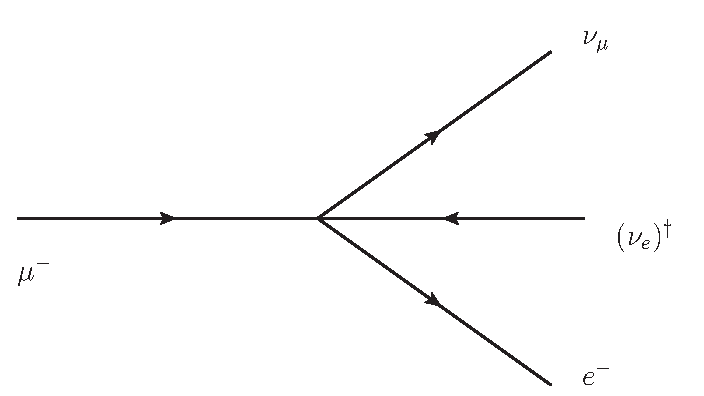
\includegraphics[scale=0.8]{mucontact}  
  \caption{Decaimiento del muón a tres cuerpos}
  \label{fig:mucontact}
\end{figure}

Construyendo la misma interacción a partir del Lagrangiano del ME
\begin{align}
  \mathcal{L}=&\frac{g_2^2}{8}\left[\bar{\nu}_\mu\gamma^\mu(1-\gamma_5)\mu\right] \left[ W_{\mu}^{+}W_\nu^{-} \right]
  \left[\bar{e}\gamma^\nu(1-\gamma_5)\nu_e\right]\,.
\end{align}
Por lo tanto la contracción apropiada de $\left[ W_{\mu}^{+}W_{\nu}^{-} \right]$ debe generar el coeficiente inverso de masa al cuadrado:
\begin{align}
  \left[ W_{\mu}^{+}W_\nu^{-} \right]\to \frac{1}{m_W^2}\,.
\end{align}
Una deducción más rigurosa se realizará en la Sección~\ref{sec:deca-debil-medi}. Por lo tanto
\begin{align}
    \frac{G_F}{\sqrt{2}}=&\frac{g^2}{8m_W^2}\nonumber\\
=& \frac{e^2}{8m_W^2\sin^2\theta_W} \nonumber\\
=& \frac{4\pi e^2}{8(4 \pi) m_W^2\sin^2\theta_W} \nonumber\\
=& \frac{\pi\alpha }{2 m_W^2\sin^2\theta_W} \nonumber\\
m_{W}^2\sin^2\theta_W=&\frac{\sqrt{2}\pi\alpha }{2 G_F} \nonumber\\
m_{W}^2\sin^2\theta_W=&\frac{\pi\alpha }{\sqrt{2} G_F} \,.
\end{align}

Además, de la ec.~\eqref{eq:mwzw}
\begin{align}
  \cos^2\theta_W=&\frac{m_W^2}{m_Z^2} \nonumber\\
  1-\sin^2\theta_W=&\frac{m_W^2}{m_Z^2} \nonumber\\
  \sin^2\theta_W=&1-\frac{m_W^2}{m_Z^2} \,.
\end{align}


De esta forma tenemos las relaciones
\begin{align}
  \sin^2\theta_W=&1-\frac{m_W^2}{m_Z^2}\,,&m_W^2\sin^2\theta_W=\frac{\pi\alpha}{\sqrt{2}G_F}\,,
\end{align}
que permiten determinar que
\begin{align}
  \sin^2\theta_W\approx &0.21\nonumber\\
  m_W\approx &81\,\text{GeV}\,.
\end{align}
El uso de $\alpha(M_Z)\approx1/128$, permite tener en cuenta algunas correcciones cuánticas dando lugar a
\begin{align}
   \sin^2\theta_W\approx &0.23\nonumber\\
  m_W\approx &80\,\text{GeV}
\end{align}
Los valores medidos son $\sin^2\theta_W=0.23149(13)$, $m_W=80.398(25)\,$GeV, y pueden ser reproducidos por el modelo estándar una vez se tienen en cuenta correcciones perturbativas inducidas por partículas virtuales.

El acelerador $e^+e^-$ LEP, que funcionó desde 1998 hasta el 2000~\cite{LEP}, operó a energías suficientes para producir millones de $Z$. Combinado con otros resultados experimentales, se pudo verificar todo el Lagrangiano del Modelo Estándar hasta un nivel del 1 por mil. Con excepción de las interacciones asociadas con el Higgs. 

La universalidad de los decaimientos del $Z$ está soportada por los resultados experimentales siguientes donde sólo se muestran los decaimientos leptónicos del $Z$ diferentes de cero \cite{a} 
\begin{align}
  \label{eq:232qft}
  \Gamma(Z\to e^+e^-)&=83.92(12)\,\text{MeV} &\Gamma(Z\to\mu^+\mu^-)&=83.99(18)\,\text{MeV} 
  &\Gamma(Z\to\tau^+\tau^-)&=84.08(22)\,\text{MeV} \nonumber\\
  \operatorname{Br}(Z\to e^+e^-)&=3.363(4)\%, &\operatorname{Br}(Z\to\mu^+\mu^-)&=3.366(7)\%,  &
  \operatorname{Br}(Z\to\tau^+\tau^-)&=3.370(8)\% 
\end{align}
Mientras que para el $W^\pm$, en \%, \cite{pdg}
\begin{align}
\label{eq:231qft}
  \operatorname{Br}(W^-\to\bar{\nu}_e e^-)&=10.71(16), &
\operatorname{Br}(W^-\to\bar{\nu}_\mu \mu^-)&=10.63(15), &
\operatorname{Br}(W^-\to\bar{\nu}_\tau \tau^-)&=11.38(21)\,. 
\end{align}
La diferencia de $\bar{\nu}_\tau \tau$ respecto a los otros representa un efecto alrededor de $2\sigma$. La universalidad de los acoplamientos leptónicos de $W$ puede comprobarse también indirectamente a través de los decaimientos débiles mediados por corrientes cargadas. Los datos actuales verifican la universalidad de los acoplamientos de corrientes cargadas leptónicas al nivel del 0.2\%~\cite{a}. Sin necesidad de entrar en detalles de los cálculos de las amplitudes de decaimiento, podemos usar el hecho de que ellas son proporcionales a los acoplamientos al cuadrado correspondiente, de modo que  un cociente entre amplitudes de decaimiento es igual, en primera aproximación, a los cocientes de los acoplamientos al cuadrado. Tendremos en cuenta además que el Branching es la amplitud de decaimiento a un canal especifico divido por la suma de las amplitudes de decaimiento a todos los canales posibles.




Para los decaimientos del $Z$ el Modelo Estándar predice, además de la ausencia de eventos del tipo $Z\to e^+\mu^-$, que para un cierto  $l=e,\mu,\tau$, o  $q=d,s,b$
\begin{align}
  \frac{ \operatorname{Br}(Z\to l^+l^-)}{ \operatorname{Br}(Z\to\bar{q}q)}\approx&
\frac{(|v_l|^2+|a_l|^2)}{N_c(|v_q|^2+|a_q|^2)}\nonumber\\
=&\frac{\left[\left(-\frac{1}{2}+2\sin^2\theta_W\right)^2+\frac{1}{4}\right]}{
N_c\left[\left(-\frac{1}{2}+\frac{2}{3}\sin^2\theta_W\right)^2+\frac{1}{4}\right]}\nonumber\\
\approx&\frac{0.776}{N_c}=
\begin{cases}
  0.338& N_c=2\\
  0.225& N_c=3\\
  0.169& N_c=4
\end{cases}
\end{align}
Para ser comparado con el resultado experimental de por ejemplo
\begin{align}
  \frac{ \operatorname{Br}(Z\to e^+e^-)}{ \operatorname{Br}(Z\to\bar{b}b)}=\frac{3.363(4)}{15.12(5)}\approx0.222
\end{align}
que de nuevo da lugar al $N_c=3$, que seguiremos tomando en adelante.

Los Branchings de decaimiento en la ec.~\eqref{eq:231qft} y ec.~\eqref{eq:232qft}  pueden ser calculados sin entrar en detalles del cálculo de las amplitudes. Teniendo en cuenta que el canal $Z\to\bar{t}t$ esta cerrado
\begin{align}
  &\operatorname{Br}(Z\to e^+e^-)=\frac{\Gamma(Z\to e^+e^-)}{\Gamma_{\text{total}}}\nonumber\\
 &\qquad=\frac{(|v_e|^2+|a_e|^2)}{\sum_l[(|v_l|^2+|a_l|^2)+(|v_{\nu_l}|^2+|a_{\nu_l}|^2)]
+N_c[\sum_{i=1}^2(|v_{u_i}|^2+|a_{u_i}|^2)+\sum_{i=1}^3(|v_{d_i}|^2+|a_{d_i}|^2)]}\nonumber\\
 &\qquad=\frac{(|v_e|^2+|a_e|^2)}{3[(|v_e|^2+|a_e|^2)+(|v_{\nu_e}|^2+|a_{\nu_e}|^2)]
+3[2(|v_{u}|^2+|a_{u}|^2)+3(|v_{d}|^2+|a_{d}|^2)]}\nonumber\\
  &\qquad=\frac{(|v_e|^2+|a_e|^2)}{21|a_e|^2+3[|v_e|^2+|v_{\nu_e}|^2]
+3[2|v_{u}|^2+3|v_{d}|^2]}\nonumber\\
 &\qquad=\frac{(-1+4s^2\theta_W)^2+1}{21+3[(-1+4s^2\theta_W)^2+1]
+3[2(1-\frac{8}{3}s^2\theta_W)^2+3(-1+\frac{4}{3}s^2\theta_W)^2]}\nonumber\\
  &\qquad=\frac{2-8s^2\theta_W+16s^4\theta_W}{42-80s^2\theta_W+\frac{320}{3}s^4\theta_W}\nonumber\\
&\qquad\approx3.43\%
\end{align}
Para $W^\pm$ tenemos por ejemplo
\begin{align}
\operatorname{Br}(W^-\to\bar{\nu}_e e^-)=\frac{\Gamma(W^-\to\bar{\nu}_e e^-)}{\Gamma_{\text{total}}}
\end{align}
donde, teniendo en cuenta que los canales a top están cerrados, y usando la condición de unitariedad de la matriz CKM en ec.~\eqref{eq:230qft}, tenemos
\begin{align}
  \Gamma_{\text{total}}=&\sum_l\Gamma(W^-\to\bar{\nu}_l l^-)+N_c\sum_i[\Gamma(W^-\to\bar{u}_1d_i)+\Gamma(W^-\to\bar{u}_2d_i)]\nonumber\\
  =&\Gamma(W^-\to\bar{\nu}_e e^-)\{3+N_c\sum_i[|V_{1i}|^2+|V_{1i}|^2]\} \nonumber\\
  =&\Gamma(W^-\to\bar{\nu}_e e^-)(3+2N_c) \nonumber\\
\end{align}
entonces
\begin{align}
  \operatorname{Br}(W^-\to\bar{\nu}_e e^-)=\frac{1}{3+2N_c}=11.1\%
\end{align}
Una mejor predicción de dichos resultados en el contexto del Modelo Estándar requiere tener en cuenta las correcciones radiativas.


El ME también tiene una predicción concreta para la amplitud del $Z$ a neutrinos, $\Gamma_{\text{inv}}$:
\begin{align}
  \frac{\Gamma_{\text{inv}}}{\Gamma_l}=&\frac{\sum_l\Gamma(Z\to\bar{\nu}_l\nu_l)}{\Gamma(Z\to e^+ e^-)}\nonumber\\
  &=\frac{N_\nu\Gamma(Z\to\bar{\nu}_e\nu_e)}{\Gamma(Z\to e^+ e^-)}\nonumber\\
  &\approx\frac{N_\nu(|v_{\nu_e}|^2+|a_{\nu_e}|^2)}{|v_{e}|^2+|a_{e}|^2}\nonumber\\
  &=\frac{2N_\nu}{(-1+4\sin^2\theta_W)^2+1}\nonumber\\
  &=\frac{N_\nu}{1-4\sin^2\theta_W+8 \sin^4\theta_W}\nonumber\\
  &\approx\begin{cases}
    5.865&N_\nu=3\\
    7.819&N_\nu=4
  \end{cases}\,,
\end{align}
mientras que el valor medido experimentalmente para esta cantidad $5.942(16)$ \cite{a}, es una evidencia muy fuerte de que sólo exiten tres neutrinos livianos. 
\end{frame}

Note que el mismo resultado se puede obtener usuando la notación de dos componentes de \eqref{eq:lsmw}. Con $t_{e_R}=0$, $t_{\nu}=-t_{e_L}=1$, $Q_{\nu}=0$ y $Q_e=-1$ tenemos que
\begin{align}
  \frac{\Gamma_{\text{inv}}}{\Gamma_l}=&\frac{\sum_l\Gamma \left[ Z\to \left( \nu_l \right)^{\dagger}\nu_l \right]}{\Gamma \left[Z\to \left( e_L \right)^{\dagger} e_L  \right]+\Gamma \left[Z\to \left( e_R \right)^{\dagger} e_R  \right]}\nonumber\\
=&\frac{N_{\nu} t_{\nu}^2 }{\left( t_{e_L} - 2 Q_e \sin^2\theta_W \right)^2+ \left( 2 Q_e \sin^2\theta_W \right)^2 } \nonumber\\
=&\frac{N_{\nu} }{\left( -1 + 2 \sin^2\theta_W \right)^2+4 \sin^4\theta_W } \nonumber\\
=&\frac{N_{\nu} }{1 - 4 \sin^2\theta_W +4 \sin^4\theta_W +4 \sin^4\theta_W } \nonumber\\
=&\frac{N_{\nu} }{1 - 4 \sin^2\theta_W +8 \sin^4\theta_W } \,.
\end{align}

\subsection{Decaimientos débiles mediados por corrientes cargadas}
\label{sec:deca-debil-medi}
\begin{frame}[fragile,allowframebreaks]
De la corrientes cargadas para leptones tenemos
\begin{align}
  \mathcal{L}_{cc}\supset&\frac{g_2}{2\sqrt{2}}\left[\sum_l\bar{\nu_l}\gamma^\mu(1-\gamma_5)l W_\mu^++\bar{l}\gamma^\mu(1-\gamma_5)\nu_l W_\mu^-\right]
\end{align}
Esto da lugar a los posibles diagramas para decaimientos de leptones a bosones virtuales, y bosones a leptontes mostrados en la figura~\ref{fig:leptoncc}. Las flechas representan el flujo de número leptónico. La flecha de tiempo es de izquierda a derecha. Al lado izquierdo del vértice entran partículas y salen antipartículas. Mientras que al lado derecho entran antip artículas y salen partículas
\begin{figure}
  \centering
  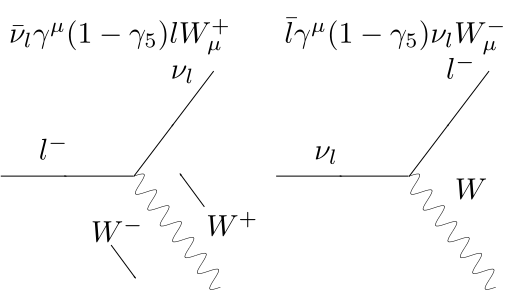
\includegraphics[scale=0.5]{leptoncc}
\qquad  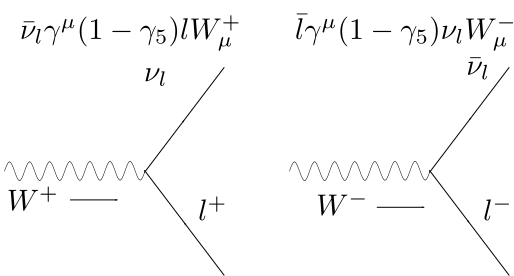
\includegraphics[scale=0.5]{wdecay}

  \caption{Diagramas de Feynman para las corrientes cargadas}
  \label{fig:leptoncc}
\end{figure}
Del primer y cuarto diagrama obtenemos el diagrama de Feynman para el decaimiento $\mu^-\to \nu_\mu e^-\bar{\nu}_e$, mostrado en la figura~\ref{fig:muondecay}
\begin{figure}
  \centering
  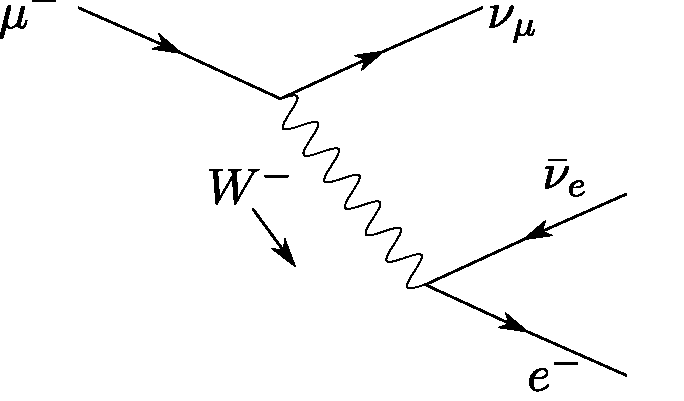
\includegraphics[scale=0.5]{muon_decay}
  \caption{diagrama de Feynman para el decaimiento $\mu^-\to \nu_\mu e^-\bar{\nu}_e$}
  \label{fig:muondecay}
\end{figure}
El propagador para el bosón $W$ de momentum $q$ resulta ser
\begin{align}
  \widetilde{D}_{\mu\nu}=\frac{1}{q^2-m_W^2}\left(g_{\mu\nu}-\frac{q_\mu q_\nu}{m_W^2}\right)\,.
\end{align}
Para los propósitos actuales la obtención de este resultado no es necesaria, el punto importante es que cuando los momentum de las partículas iniciales y finales son mucho más pequeñas que $m_W$, esto se reduce a
\begin{align}
  \widetilde{D}_{\mu\nu}=-\frac{g_{\mu\nu}}{m_W^2}\,.
\end{align}
Este resultado se entiende fácilmente cuando se compara con el propagador de una partículas escalar masiva $1/(q^2-M^2)\to-1/M^2$. Las componentes espaciales de $W_\mu$ con $\mu=1,2,3$, a bajas energías tienen el mismo propagador que el de una partícula escalar, mientras $W_0$, tiene el signo opuesto.

El Lagrangiano efectivo para el decaimiento del muón, $\mu^-\to \nu_\mu e^- \bar{\nu}_e$ es entonces
\begin{align}
  \mathcal{L}=&\frac{g_2^2}{8}\left[\bar{\nu}_\mu\gamma^\mu(1-\gamma_5)\mu\right]\frac{g_{\mu\nu}}{m_W^2}
  \left[\bar{e}\gamma^\nu(1-\gamma_5)\nu_e\right]\nonumber\\
=&\frac{g_2^2}{8m_W^2}\left[\bar{\nu}_\mu\gamma^\mu(1-\gamma_5)\mu\right]
  \left[\bar{e}\gamma^\nu(1-\gamma_5)\nu_e\right]\nonumber\\
  =&\frac{G_F}{\sqrt{2}}\left[\bar{\nu}_\mu\gamma^\mu(1-\gamma_5)\mu\right]\left[\bar{e}\gamma_\mu(1-\gamma_5)\nu_e\right]\,,
\end{align}
donde
\begin{align}
  \frac{G_F}{\sqrt{2}}=&\frac{g_2^2}{8m_W^2}\nonumber\\
  =&\frac{g_2^24}{8g^2v^2}\nonumber\\
  =&\frac{1}{2v^2}\,,
\end{align}
y
\begin{align}
  v=\left(\sqrt{2}\,G_F\right)^{-1/2}=&246.2\ \text{GeV}\nonumber\\
 \approx&2.9\times 10^{15}\ \text{K} \nonumber\\
 \approx&4.9\times 10^{-14}\ \text{m} \nonumber\\
 \approx&1.6\times 10^{-22}\ \text{s} \,.
\end{align}


De otro lado, para el  decaimiento $\beta$, $n\to p e^- \bar{\nu}_e$, de acuerdo a la figura~\ref{fig:neutrondecay}, tenemos

\begin{align}
    \mathcal{L}=\frac{G_\beta}{\sqrt{2}}\left[\bar{p}\gamma^\mu(1-1.26\gamma_5)n\right]\left[\bar{e}\gamma_\mu(1-\gamma_5)\nu_e\right]\,.
\end{align}
\begin{figure}
  \centering
  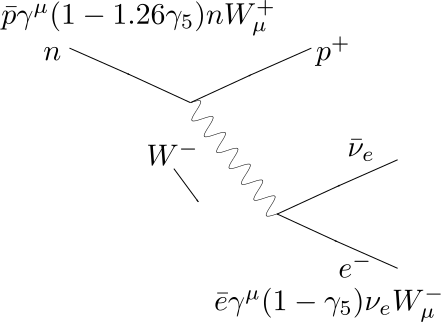
\includegraphics[scale=0.5]{neutrondecay}
  \caption{Decaimiento del neutrón.}
  \label{fig:neutrondecay}
\end{figure}
con $G_F$ dado en la ec.~\eqref{eq:233qft} y $G_\beta=1.10\times 10^{-5}\,\text{GeV}^2$. La corriente hadrónica tiene la forma V--1.26A. El factor 1.26  puede entenderse como debido a las correcciones a nivel hadrónico de una corriente que es de la forma V--A a nivel del quarks, como en la ec.~\eqref{eq:234qft}. A nivel de quarks el decaimiento del neutrón ($udd$) al protón ($uud$) corresponde al decaimiento de uno de los quarks down del neutrón $d\to u e^- \bar{\nu}_e$
\begin{align}
    \mathcal{L}=\frac{G_F}{\sqrt{2}}V_{11}\left[\bar{u}\gamma^\mu(1-\gamma_5)d\right]\left[\bar{e}\gamma_\mu(1-\gamma_5)\nu_e\right]\,.
\end{align}
De modo que $G_\beta=G_F V_{11}=G_F\cos\theta_C$, donde $\theta_C$ es el ángulo de Cabbibo. Una vez se tienen en cuenta correcciones electrodébiles se obtiene el valor $|V_{11}|=0.97418(27)$\cite{PDG}. Las magnitudes de los elementos de la matriz CKM son\cite{PDG}
\begin{align}
  V\approx\begin{pmatrix}
    0.97419&0.2257&0.0359\\
    0.2256&0.97334&0.0415\\
    0.00874&0.0407&0.999133
  \end{pmatrix}\sim \mathbf{1}
\end{align}
\end{frame}

Para cerrar esta notas, transcribo a continuación el último párrafo de la conferencia de Steven Weinberg en 1979 con motivo de la entrega del premio nobel del física por el desarrollo del modelo estándar de las interacciones fundamentales:

\begin{quote}
[...]  And
nothing makes me more optimistic than the discovery of broken symmetries.
In the seventh book of the Republic, Plato describes prisoners who are
chained in a cave and can see only shadows that things outside cast on the
cave wall. When released from the cave at first their eyes hurt, and for a
while they think that the shadows they saw in the cave are more real than
the objects they now see. But eventually their vision clears, and they can
understand how beautiful the real world is. We are in such a cave, imprisoned
by the limitations on the sorts of experiments we can do. In particular,
we can study matter only at relatively low temperatures, where symmetries
are likely to be spontaneously broken, so that nature does not appear
very simple or unified. We have not been able to get out of this cave, but by
looking long and hard at the shadows on the cave wall, we can at least make
out the shapes of symmetries, which though broken, are exact principles
governing all phenomena, expressions of the beauty of the world outside.
\end{quote}
S. Weinberg, Nobel lecture, 1979

\section{Resumen}
A modo de resumén, usaremos a continuación la siguiente secuencia de la historieta de \url{http://www.phdcomics.com} re-explicando el bosón de Higgs:
\newpage

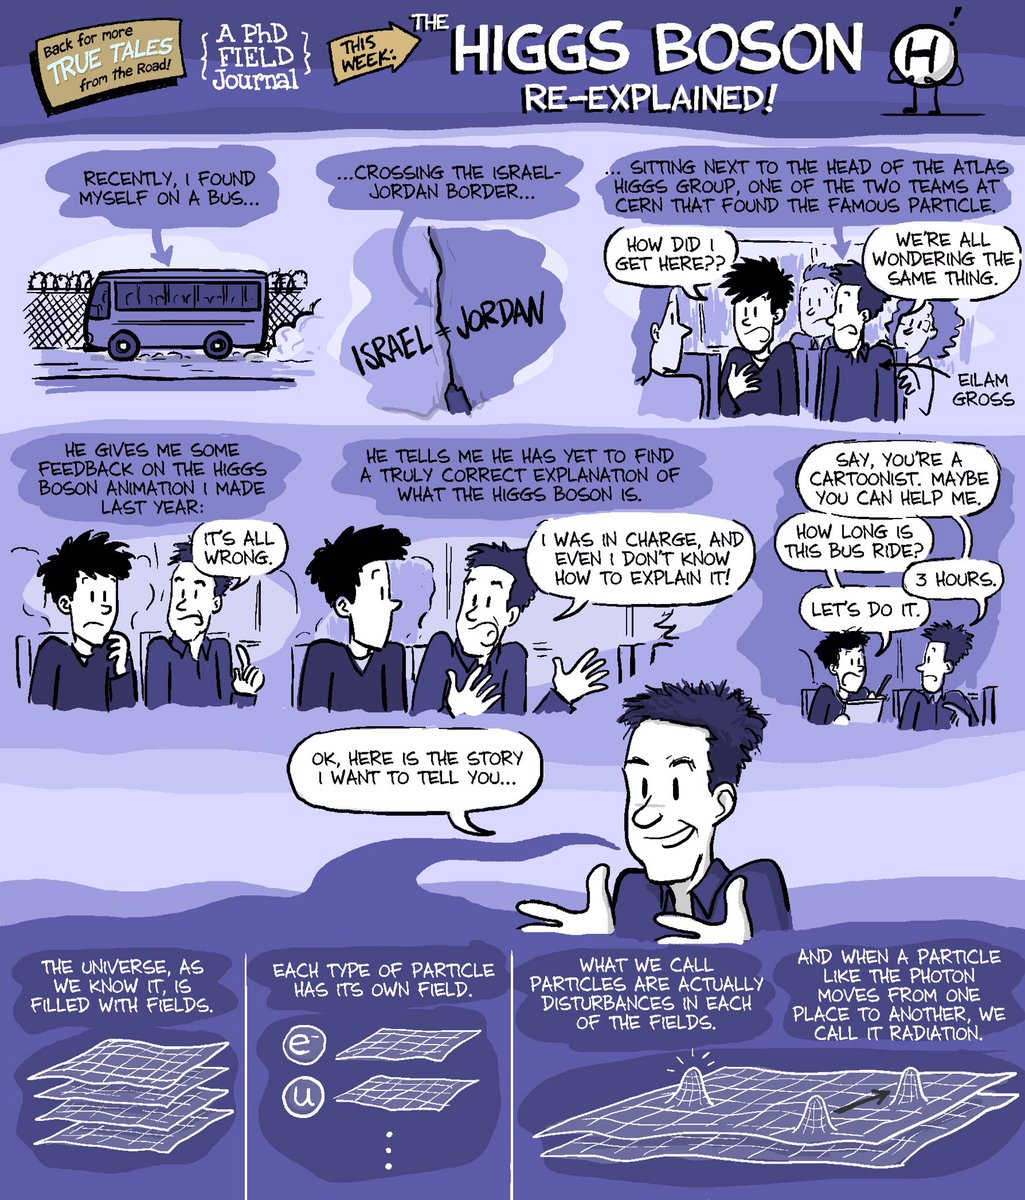
\includegraphics[scale=0.51]{Higgs1}

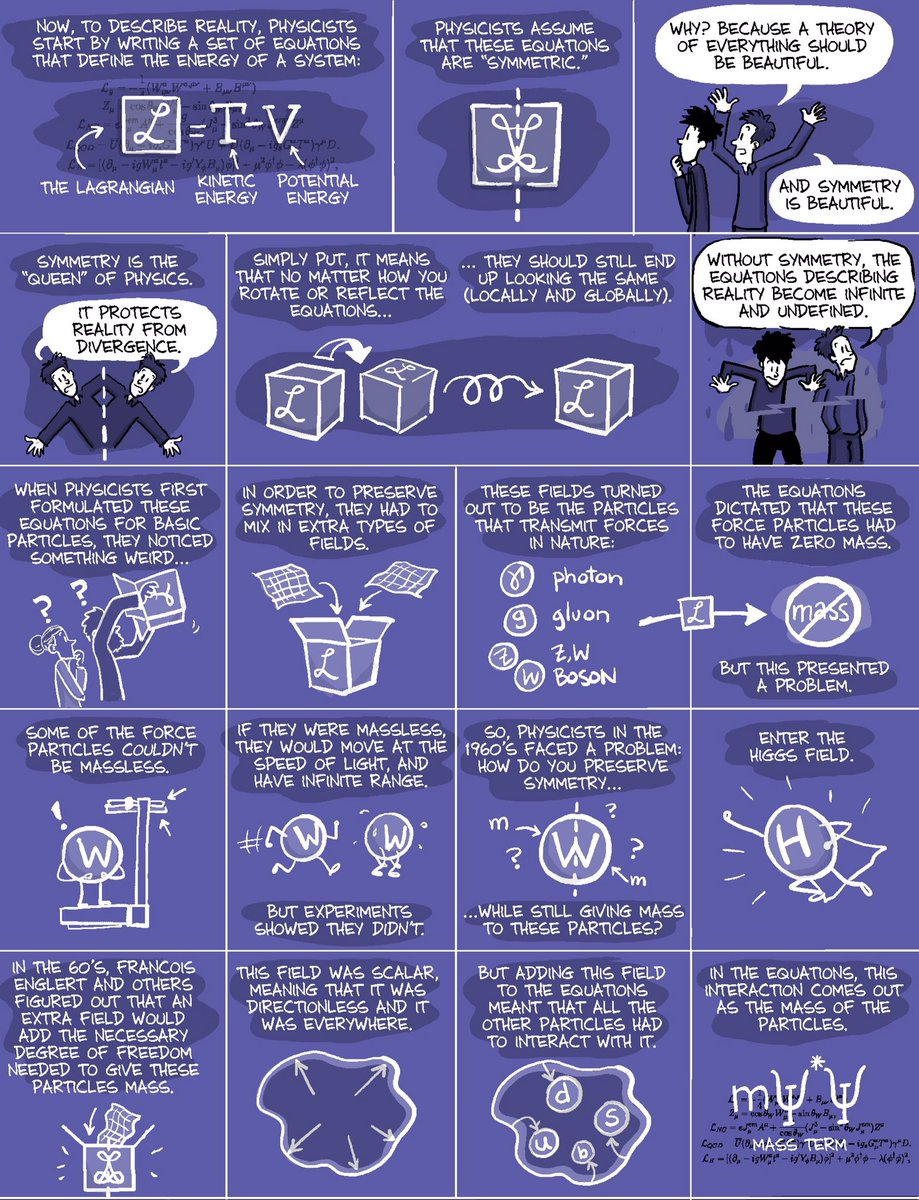
\includegraphics[scale=0.56]{Higgs2}

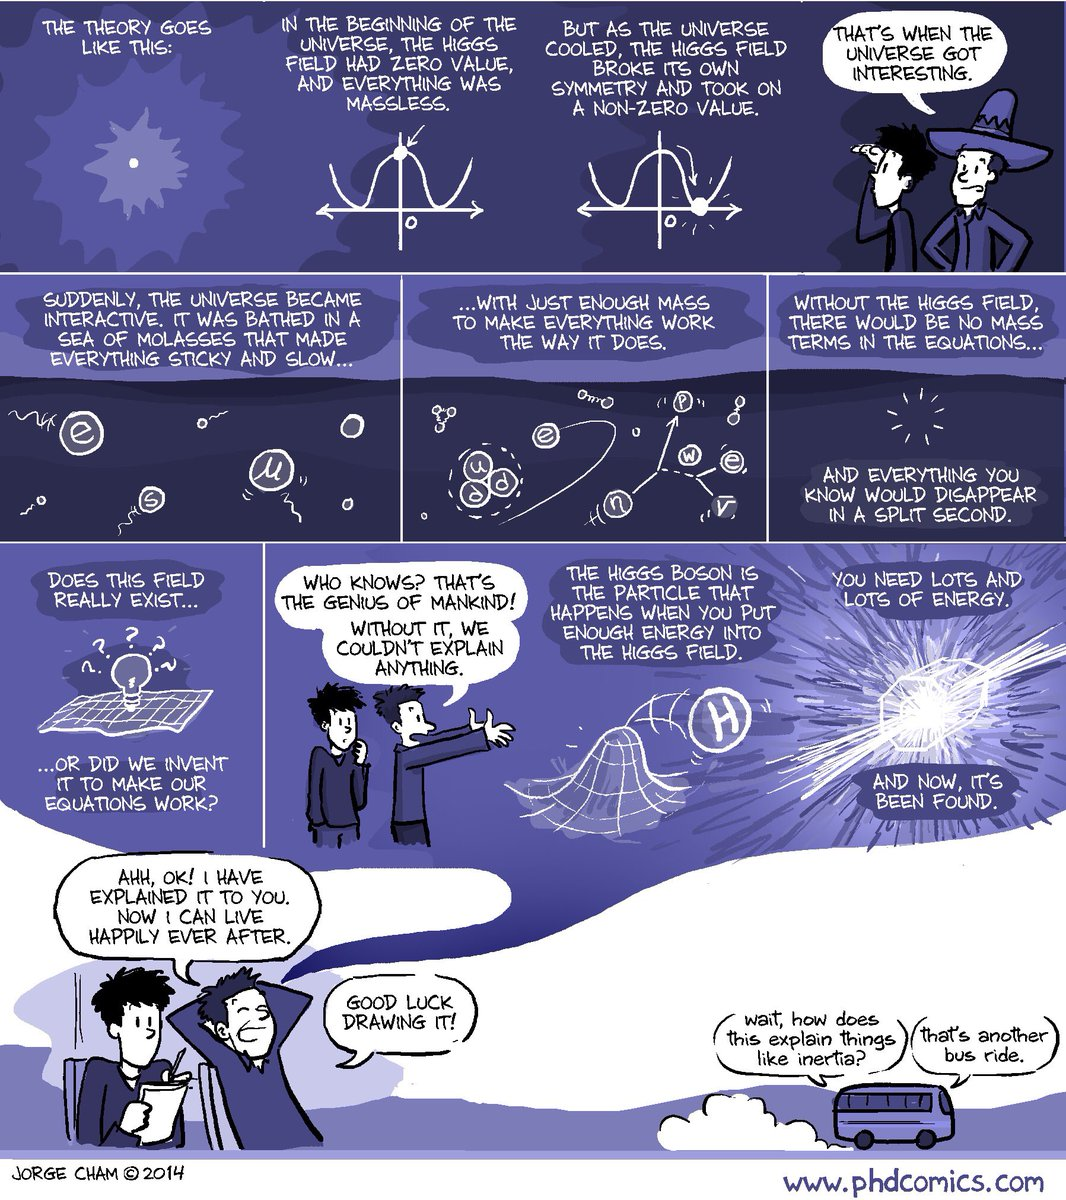
\includegraphics[scale=0.49]{Higgs3}

\newpage


\section{Lecturas recomendadas}
Libros:
\begin{itemize}
\item \cite{kane,cottingham,Pich:2005mk}
\end{itemize}

Artículos originales

\begin{itemize}
\item Teorías no abelianas \cite{Yang:1954ek}
\item Mecanismo de Higgs \cite{Higgs:1964pj}
\item Teoría electrodébil \cite{Weinberg:1967tq}
\end{itemize}

Artículo de divulgación
\begin{itemize}
\item The deconstructed Standard Model equation, Rashmi Shivni \url{https://www.symmetrymagazine.org/article/the-deconstructed-standard-model-equation}
\end{itemize}

Videos:
\begin{itemize}
\item Strange Stars Explained: \url{https://www.youtube.com/watch?v=p_8yK2kmxoo}
\end{itemize}

% \left(\right)
%
%%% Local Variables: 
%%% mode: latex
%%% TeX-master: "fullnotes"
%%% ispell-local-dictionary: "castellano8"
%%% End:
}

\end{document}

%TEMPLATES:

\chapter{Hola}
\section{Introduction}
This is the introduction text. This text is not shown in the
presentation, but will be part of the article.
\begin{frame}
Hola mundo
\end{frame}
This text is once more not shown in the presentation.
\section{Main Part}
While this text is not shown in the presentation, the section command
also applies to the presentation.
We can add a subsection that is only part of the article like this:
\subsection<article>{Article-Only Section}
With some more text.
\begin{frame}
This text is part both of the article and of the presentation.
\begin{itemize}
\item This stuff is also shown in both version.
\item This too.
\only<article>{\item This particular item is only part
of the article version.}
\item<presentation:only@0> This text is also only part of the article.
\end{itemize}

\end{frame}

Templates:
%%%tablas de colores
\mode<presentation>{\rowcolors{1}{RoyalBlue!20}{}}

\begin{frame}[fragile,allowframebreaks]
\end{frame}

%numbers in beamer
\begin{lstlisting}[numbers=left,xleftmargin=1cm,numberstyle=\tiny,escapeinside={(*}{*)}]
\end{lstlisting}


\begin{pyprogram}
\lstset{numbers=left}
\begin{lstlisting}[label=XXX,caption=XXX]
\end{lstlisting}
\end{pyprogram}

\begin{pyprogram}
\mode<presentation>{\lstset{basicstyle=\tiny\ttfamily}}
\filetitle{cinematica.py}
\lstinputlisting{python/programas/cinematica/cinematica.py}
\end{pyprogram}



\begin{ipython}
\begin{lstlisting}[title=]
In [1]:
\end{lstlisting}
\end{ipython}

\begin{terminal}
\begin{lstlisting}[title=1]

\end{lstlisting}
\end{terminal}

\begin{columns}
  \begin{column}{0.5\textwidth}
    
  \end{column}
  \begin{column}{0.5\textwidth}
    
  \end{column}
\end{columns}


%%% Local Variables: 
%%% mode: latex
%%% TeX-master: "beyond.beamer.tex"
%%% End: 
